%% LyX 2.3.2 created this file.  For more info, see http://www.lyx.org/.
%% Do not edit unless you really know what you are doing.
\documentclass[oneside,english]{manual}
\usepackage[scaled=0.7]{beramono}
\usepackage[T1]{fontenc}
\usepackage[latin9]{inputenc}
\setcounter{tocdepth}{3}
\usepackage{color}
\usepackage{babel}
\usepackage{amsmath}
\usepackage{makeidx}
\makeindex
\usepackage{graphicx}
\usepackage[authoryear]{natbib}
\usepackage[unicode=true,
 bookmarks=true,bookmarksnumbered=false,bookmarksopen=true,bookmarksopenlevel=1,
 breaklinks=true,pdfborder={0 0 1},backref=page,colorlinks=true]
 {hyperref}
\hypersetup{pdftitle={simuPOP User's Guide},
 pdfauthor={Bo Peng},
 pdfkeywords={simuPOP},
 linkcolor=TitleColor,urlcolor=LinkColor}

\makeatletter
%%%%%%%%%%%%%%%%%%%%%%%%%%%%%% User specified LaTeX commands.
\renewcommand{\py@ptsize}{12pt}

\setreleaseinfo{Release 1.1.7 (\mbox{Rev: 5000})}
% file revision $Rev: 3372$
\authoraddress{
{\bf Department of Epidemiology, U.T. M.D. Anderson Cancer Center}\\
{\bf Email: } \textsf{bpeng@mdanderson.org}\\
{\bf URL: } \textsf{http://simupop.sourceforge.net} \\
{\bf Mailing List: } \textsf{simupop-list@lists.sourceforge.net}
}
\author{Bo Peng}
\date{December 2004\\
\hfill{}\\
Last modified \\
\today }

\ifhtml
\chapter*{Front Matter\label{front}}
\fi

\usepackage{listings}
\renewcommand{\lstlistlistingname}{List of Examples}
\renewcommand{\lstlistingname}{Example}

\sloppy

\definecolor{TitleColor}{rgb}{0.126,0.263,0.361}
\definecolor{LinkColor}{rgb}{0.208,0.374,0.486}
\definecolor{VerbatimColor}{rgb}{0,0,0}
\definecolor{VerbatimBackgroundColor}{rgb}{0.98,0.941,0.902}
\definecolor{VerbatimBorderColor}{rgb}{0,0,0}
\definecolor{VerbatimStringColor}{rgb}{0,0.5,0}
\definecolor{VerbatimCommentColor}{rgb}{0.2,0.2,0.2}
\definecolor{VerbatimPromptColor}{rgb}{0.588,0.098,0.054}

\usepackage{sectsty}
\sectionfont{\color{TitleColor}}
\subsectionfont{\color{TitleColor}}
\subsubsectionfont{\color{TitleColor}}

\makeatother

\usepackage{listings}
\lstset{alsoletter={>.},
backgroundcolor={\color{VerbatimBackgroundColor}},
basicstyle={\ttfamily\color{VerbatimColor}},
commentstyle={\small\color{VerbatimCommentColor}\slshape},
emph={[2]>>>,...},
emphstyle={[2]\color{VerbatimPromptColor}\bf},
language=Python,
otherkeywords={>>>,...},
showspaces=false,
showstringspaces=false,
showtabs=false,
stringstyle={\color{VerbatimStringColor}},
xleftmargin=10pt}
\renewcommand{\lstlistingname}{Listing}

\begin{document}
\title{simuPOP User's Guide}

\maketitle
\noindent\begin{minipage}[c][1\totalheight]{1\columnwidth}%
\vspace{7.5in} 

 \copyright{}  2004-2008 Bo Peng \vspace{.3cm} \hrule \vspace{0.1cm} Permission
is granted to make and distribute verbatim copies of this manual provided
the copyright notice and this permission notice are preserved on all
copies. Permission is granted to copy and distribute modified versions
of this manual under the conditions for verbatim copying, provided
also that the sections entitled Copying and GNU General Public License
are included exactly as in the original, and provided that the entire
resulting derived work is distributed under the terms of a permission
notice identical to this one. Permission is granted to copy and distribute
translations of this manual into another language, under the above
conditions for modified versions, except that this permission notice
may be stated in a translation approved by the Free Software Foundation.%
\end{minipage}
\begin{abstract}
simuPOP is a general-purpose individual-based forward-time population
genetics simulation environment. Unlike coalescent-based programs,
simuPOP evolves populations forward in time, subject to arbitrary
number of genetic and environmental forces such as mutation, recombination,
migration and Population/subpopulation size changes. In contrast to
competing applications that use command-line options or configuration
files to direct the execution of a limited number of predefined evolutionary
scenarios, users of simuPOP\textquoteright s scripting interface could
make use of many of its unique features, such as customized chromosome
types, arbitrary nonrandom mating schemes, virtual subpopulations,
information fields and Python operators, to construct and study almost
arbitrarily complex evolutionary scenarios. 

simuPOP is provided as a number of Python modules, which consist of
a large number of Python objects and functions, including population,
mating schemes, operators (objects that manipulate populations) and
simulators to coordinate the evolutionary processes. It is the users\textquoteright{}
responsibility to write a Python script to glue these pieces together
and form a simulation. At a more user-friendly level, an increasing
number of functions and scripts contributed by simuPOP users is available
in the online simuPOP cookbook. They provide useful functions for
different applications (e.g. load and manipulate HapMap samples, import
and export files from another application) and allow users who are
unfamiliar with simuPOP to perform a large number of simulations ranging
from basic population genetics models to generating datasets under
complex evolutionary scenarios.

This user's guide shows you how to install and use simuPOP using a
large number of examples. It describes all important concepts and
features of simuPOP and demonstrates how to use them in a simuPOP
script. Although the new Python 3.x releases are incompatible with
Python 2.x, examples in this book are written in a style that is compatible
with both versions of Python. For a complete and detailed description
about all simuPOP functions and classes, please refer to the \emph{simuPOP
Reference Manual}. All resources, including a pdf version of this
guide and a mailing list can be found at the simuPOP homepage \texttt{http://simupop.sourceforge.net}.

\textbf{How to cite simuPOP:}

\begin{quote}
Bo Peng and Marek Kimmal (2005) simuPOP: a forward-time population
genetics simulation environment. \emph{bioinformatics}, \textbf{21}
(18): 3686-3687

Bo Peng and Christopher Amos (2008) Forward-time simulations of nonrandom
mating populations using simuPOP. \emph{bioinformatics}, \textbf{24}
(11) 1408-1409.
\end{quote}
\end{abstract}
\tableofcontents{}

\lstlistoflistings

\listoffigures


\chapter{Introduction}

\section{What is simuPOP?}

simuPOP is a \textbf{general-purpose individual-based forward-time
population genetics simulation environment} based on Python, a dynamic
object-oriented programming language that has been widely used in
biological studies. More specifically,
\begin{itemize}
\item simuPOP is a \textbf{population genetics simulator} that simulates
the evolution of populations. It uses a discrete generation model
although overlapping generations could be simulated using nonrandom
mating schemes. 
\item simuPOP explicitly models \textbf{populations with individuals} who
have their own genotype, sex, and auxiliary information such as age.
The evolution of a population is modeled by populating an offspring
population from parents in the parental population.
\item Unlike coalescent-based programs, simuPOP evolves populations \textbf{forward
in time}, subject to arbitrary number of genetic and environmental
forces such as mutation, recombination, migration and Population/subpopulation
size changes.
\item simuPOP is a \textbf{general-purpose} simulator that is designed to
simulate arbitrary evolutionary processes. In contrast to competing
applications that use command-line options or configuration files
to direct the execution of a limited number of predefined evolutionary
scenarios, users of simuPOP\textquoteright s scripting interface could
make use of many of its unique features, such as customized chromosome
types, arbitrary nonrandom mating schemes, virtual subpopulations,
information fields and Python operators, to construct and study almost
arbitrarily complex evolutionary scenarios. In addition, because simuPOP
provides a large number of functions to manipulate populations, it
can be used as an data manipulatation and analysis tool.
\end{itemize}
simuPOP is provided as a number of Python modules, which consist of
a large number of Python objects and functions, including Population,
mating schemes, operators (objects that manipulate populations) and
simulators to coordinate the evolutionary processes. It is the users\textquoteright{}
responsibility to write a Python script to glue these pieces together
and form a simulation. At a more user-friendly level, an increasing
number of functions and scripts contributed by simuPOP users is available
in the online simuPOP cookbook (\texttt{http://simupop.sourceforge.net/cookbook}).
They provide useful functions for different applications (e.g. load
and manipulate HapMap samples, import and export files from another
application) and allow users who are unfamiliar with simuPOP to perform
a large number of simulations ranging from basic population genetics
models to generating datasets under complex evolutionary scenarios.

\section{An overview of simuPOP concepts}

A simuPOP \textbf{population} consists of \textbf{individuals} of
the same \textbf{genotype structure}, which includes properties such
as number of homologous sets of chromosomes (ploidy), number of chromosomes,
and names and locations of markers on each chromosome. In addition
to basic information such as genotypes and sex, individuals can have
arbitray auxillary values as \textbf{information fields}. Individuals
in a population can be divided into \textbf{subpopulations} that can
be further grouped into \textbf{virtual subpopulations} according
to individual properties such as sex, affection status, or arbitrary
auxiliary information such as age. Whereas subpopulations define boundaries
of individuals that restrict the flow of individuals and their genotypes
(mating happens within subpopulations), virtual subpopulations are
groups of individuals who share the same properties, with membership
of individuals change easily with change of individual properties.

\begin{figure}[h]
\caption{\label{fig:life-cycle}A life cycle of an evolutionary process}

\begin{centering}
\includegraphics[width=0.8\textwidth]{figures/evolve}
\par\end{centering}
\centering{}Illustration of the discrete-generation evolutionary model
used by simuPOP.
\end{figure}

\textbf{Operators} are Python objects that act on a population. They
can be applied to a population before or after mating during a life
cycle of an evolutionary process (Figure \ref{fig:life-cycle}), or
to parents and offspring during the production of each offspring.
Arbitrary numbers of operators can be applied to an evolving population.

A simuPOP \textbf{mating scheme} is responsible for choosing parent
or parents from a parental (virtual) subpopulation and for populating
an offspring subpopulation. simuPOP provides a number of pre-defined
\textbf{homogeneous mating schemes}, such as random, monogamous or
polygamous mating, selfing, and haplodiploid mating in hymenoptera.
More complicated nonrandom mating schemes such as mating in age-structured
populations can be constructed using \textbf{heterogeneous mating
schemes}, which applies multiple homogeneous mating schemes to different
(virtual) subpopulations.

simuPOP evolves a population generation by generation, following the
evolutionary cycle depicted in Figure \ref{fig:life-cycle}. Briefly
speaking, a number of \textbf{operators} such as a \texttt{KAlleleMutator}
are applied to a population before a mating scheme repeatedly chooses
a parent or parents to produce offspring. \textbf{During-mating operators}
such as \texttt{Recombinator} can be applied by a mating scheme to
transmit parental genotype to offspring. After an offspring population
is populated, other \textbf{operators} can be applied, for example,
to calculate and output population statistics. The offspring population
will then become the parental population of the next evolutionary
cycle. Many simuPOP operators can be applied in different stages so
the type of an operator is determined by the stage at which it is
applied. Several populations, or replicates of a single population,
could form a \textbf{simulator} and evolve together.

\lstinputlisting[caption={A simple example},label={simple-example}]{log/simpleExample.log}

Some of these concepts are demonstrated in Example \ref{simple-example},
where a standard diploid Wright-Fisher model with recombination is
simulated. The first line imports the standard simuPOP module. The
second line creates a diploid population with 1000 individuals, each
having one chromosome with two loci. The \texttt{evolve()} function
evolves the population using a random mating scheme and four operators.

Operators \texttt{InitSex} and \texttt{InitGenotype} are applied at
the beginning of the evolutionary process. Operator \texttt{InitSex}
initializes individual sex randomly and \texttt{InitGenotype} initializes
all individuals with the same genotype \texttt{12/21}. The populations
are then evolved for 100 generations. A random mating scheme is used
to generate offspring. Instead of using the default Mendelian genotype
transmitter, a \texttt{Recombinator} (during-mating operator) is used
to recombine parental chromosomes with the given recombination rate
\texttt{0.01} during the generation of offspring. The other operators
are applied to the offspring generation (post-mating) at every 10
generations (parameter \texttt{step}). Operator \texttt{Stat} calculates
linkage disequilibrium between the first and second loci. The results
of this operator are stored in a local variable space of the Population.
The last operator \texttt{PyEval} outputs calculated linkage disequilibrium
values with a trailing new line. The result represents the decay of
linkage disequilibrium of this population at 10 generation intervals.
The return value of the \texttt{evolve} function, which is the number
of evolved generations, is also printed.

\section{Features}

simuPOP offers a long list of features, many of which are unique among
all forward-time population genetics simulation programs. The most
distinguishing features include:
\begin{enumerate}
\item simuPOP provides three types of modules that use 1, 8 or 32/64 bits
to store an allele. The binary module (1 bit) is suitable for simulating
a large number of SNP markers, and the long module (32 or 64 bits
depending on platform) is suitable for simulating some population
genetics models such as the infinite allele mutation model.
\item {[}NEW in simuPOP 1.0.7{]} simuPOP provides modules to store a large
number of rare variants in a compressed manner (the mutant module),
and to store origin of each allele so that it is easy to track allelic
lineage during evolution.
\item The core of simuPOP is implemented in C++ which is heavily optimized
for large-scale simulations. simuPOP can be executed in multiple threads
with boosted performance on modern multi-core CPUs. 
\item In addition to autosomes and sex chromosomes, simuPOP supports arbitrary
types of chromosomes through customizable genotype transmitters. Random
maternal transmission of mitochondrial DNAs is supported as a special
case of this feature.
\item An arbitrary number of float numbers, called \textbf{information fields},
can be attached to individuals of a population. For example, information
field \texttt{father\_idx} and \texttt{mother\_idx} can be used to
track an individual\textquoteright s parents, and \texttt{pack\_year}
can be used to simulate an environmental factor associated with smoking.
\item simuPOP does not impose a limit on the number of homologous sets of
chromosomes, the size of the genome or populations. The size of your
simulation is only limited by the physical memory of your computer.
\item During an evolutionary process, a population can hold more than one
most-recent generation. Pedigrees can be sampled from such multi-generation
populations.
\item An operator can be native (implemented in C++) or hybrid (Python-assisted).
A hybrid operator calls a user-provided Python function to implement
arbitrary genetic effects. For example, a hybrid mutator passes to-be-mutated
alleles to a function and mutates these alleles according to the returned
values. 
\item simuPOP provides more than 60 operators that cover all important aspects
of genetic studies. These include mutation (\emph{e.g. k}-allele,
stepwise, generalized stepwise and context-sensitive mutation models),
migration (arbitrary, can create new subpopulation), recombination
and gene conversion (uniform or nonuniform), selection (single-locus,
additive, multiplicative or hybrid multi-locus models, support selection
of both parents and offspring), penetrance (single, multi-locus or
hybrid), ascertainment (case\textendash control, affected sibpairs,
random, nuclear and large Pedigrees), statistics calculation (including
but not limited to allele, genotype, haplotype, heterozygote number
and frequency; linkage disequilibrium measures, Hardy-Weinberg test),
pedigree tracing, visualization (using R or other Python modules)
and load/save in simuPOP\textquoteright s native format and many external
formats such as Linkage.
\item Mating schemes can work on virtual subpopulations of a subpopulation.
For example, positive assortative mating can be implemented by mating
individuals with similar properties such as ancestry and overlapping
generations could be simulated by copying individuals acorss generations.
The number of offspring per mating event can be fixed or can follow
a statistical distribution. 
\end{enumerate}
A number of forward-time simulation programs are available. If we
exclude early forward-time simulation applications developed primarily
for teaching purposes, notable forward-time simulation programs include
\emph{easyPOP}, \emph{FPG}, \emph{Nemo} and \emph{quantiNemo}, \emph{genoSIM}
and \emph{genomeSIMLA}, \emph{FreGene}, \emph{GenomePop}, \emph{ForwSim},
and \emph{ForSim}. These programs are designed with specific applications
and specific evolutionary scenarios in mind, and excel in what they
are designed for. For some applications, these programs may be easier
to use than simuPOP. For example, using a special look-ahead algorithm,
\emph{ForwSim} is among the fastest programs to simulate a standard
Wright-Fisher process, and should be used if such a simulation is
needed. However, these programs are not flexible enough to be applied
to problems outside of their designed application area. For example,
none of these programs can be used to study the evolution of a disease
predisposing mutant, a process that is of great importance in statistical
genetics and genetic epidemiology. Compared to such programs, simuPOP
has the following advantages:
\begin{itemize}
\item The scripting interface gives simuPOP the flexibility to create arbitrarily
complex evolutionary scenarios. For example, it is easy to use simuPOP
to explicitly introduce a disease predisposing mutant to an evolving
population, trace the allele frequency of them, and restart the simulation
if they got lost due to genetic drift.
\item The Python interface allows users to define customized genetic effects
in Python. In contrast, other programs either do not allow customized
effects or force users to modify code at a lower (e.g. C++) level.
\item simuPOP is the only application that embodies the concept of virtual
subpopulation that allows evolutions at a finer scale. This is required
for realistic simulations of complex evolutionary scenarios.
\item simuPOP allows users to examine an evolutionary process very closely
because all simuPOP objects are Python objects that can be assessed
using their member functions. For example, users can keep track of
genotype at particular loci during evolution. In contrast, other programs
work more or less like a black box where only limited types of statistics
can be outputted.
\end{itemize}

\section{License, Distribution and Installation}

simuPOP is distributed under a GPL license and is hosted at\texttt{
http://simupop.sourceforge.net}, the world's largest development and
download repository of Open Source code and applications. simuPOP
is available on any platform where Python is available, and is currently
tested under both 32 and 64 bit versions of Windows (Windows 2000
and later), Linux (Redhat and Ubuntu), MacOS X and Sun Solaris systems.
Different C++ compilers such as Microsoft Visual C++, gcc and Intel
icc are supported under different operating systems. Standard installation
packages are provided for Windows, Linux, and MacOS X systems.

If a binary distribution is unavailable for a specific platform, it
is usually easy to compile simuPOP from source, following the standard
\texttt{``python setup.py install''} procedure. Please refer to
the \texttt{installation} section of the simupop website for instructions
for specific platforms and compilers.

simuPOP is available for Python 2.4 and later, including the new Python
3.x releases. Although Python 3 is incompatible with Python 2 in many
ways, examples in this guide are written in a style that is compatible
with both versions of Python. Some non-classic usages include the
use of \texttt{a//b} instead of \texttt{a/b} for floored division
and \texttt{list(range(3))} instead of \texttt{range(3)} for sequece
\texttt{{[}0,1,2{]}} In particular, we use 
\begin{lstlisting}
print("Population size is %d" % size)
\end{lstlisting}
 instead of 
\begin{lstlisting}
print "Population size is %d" % size
\end{lstlisting}
 to output strings because the former is valid in Python 2.x (print
a tuple with one element) and will generate the same output in Python
3.x. Of course, users of simuPOP can choose to use other styles.

Thanks to the \textquoteleft glue language\textquoteright{} nature
of Python, it is easy to inter-operate with other applications within
a simuPOP script. For example, users can call any R function from
Python/simuPOP for the purposes of visualization and statistical analysis,
using \texttt{R} and a Python module \texttt{RPy}. Because simuPOP
utility modules such as \texttt{simuPOP.plotter} and \texttt{simuPOP.sampling}
makes use of \texttt{R} and \texttt{rpy} (not \texttt{rpy2}) to plot
figures, \textbf{it is hihgly recommended that you install R and RPy
with simuPOP}. In addition, although simuPOP uses the standard \texttt{Tkinter}
GUI toolkit when a graphical user interface is needed, it can make
use of a \texttt{wxPython} toolkit if it is available.

\section{How to read this user's guide}

This user's guide describes all simuPOP features using a lot of examples.
The first few chapters describes all classes in the simuPOP core.
Chapter \ref{cha:simuPOP-Operators} describes almost all simuPOP
operators, divided largely by genetic models. Features listed in these
two chapters are generally implemented at the C++ level and are provided
through the \texttt{simuPOP} module. Chapter \ref{cha:Utility-Modules}
describes features that are provided by various simuPOP utility modules.
These modules provide extensions to the simuPOP core that improves
the usability and userfriendliness of simuPOP. The next chapter (Chapter
\ref{cha:A-real-example}) demonstrates how to write a script to solve
a real-world simulation problem. Because some sections describe advanced
features that are only used in the construction of highly complex
simulations, or implementation details that concern only advanced
users, new simuPOP users can safely skip these sections. \textbf{Sections
that describe advanced topics are marked by one or two asterisks ({*})
after the section} \textbf{titles}.

simuPOP is a comprehensive forward-time population genetics simulation
environment with many unique features. If you are new to simuPOP,
you can go through this guide quickly and understand what simuPOP
is and what features it provides. Then, you can read Chapter \ref{cha:A-real-example}
and learn how to apply simuPOP in real-world problems. After you play
with simuPOP for a while and start to write simple scripts, you can
study relevant sections in details. The \emph{simuPOP reference manual}
will become more and more useful when the complexity of your scripts
grows.

Before we dive into the details of simuPOP, it is helpful to know
a few name conventions that simuPOP tries to follow. Generally speaking,
\begin{itemize}
\item All class names use the CapWords convention (e.g. \texttt{Population()},
\texttt{InitSex()}) .
\item All standalone functions (e.g. \texttt{loadPopulation()} and \texttt{initSex()}),
member functions (e.g. \texttt{Population.mergeSubPops()}) and parameter
names use the mixedCases style.
\item Constants are written in all capital characters with underscores separating
words (e.g. \texttt{CHROMOSOME\_X}, \texttt{UNIFORM\_DISTRIBUTION}).
Their names instead of their actual values should be used because
those values can change without notice.
\item simuPOP uses the abbreviated form of the following words in function
and parameter names:

\begin{quote}
\texttt{pop} (population), \texttt{pops} (populations), \texttt{pos}
(position),  \texttt{info} (information), \texttt{migr} (migration),
\texttt{subPop} (subpopulation and virtual subpopulation), \texttt{subPops}
(subpopulations and virtual subpopulations), \texttt{rep} (replicates),
\texttt{gen} (generation), \texttt{ops} (operators), \texttt{expr}
(expression), \texttt{stmts} (statements).
\end{quote}
\item simuPOP uses both singular and plural forms of parameters, according
to the following rules:

\begin{itemize}
\item If a parameter only accept a single input, singular names such as
\texttt{field}, \texttt{locus}, \texttt{value}, and \texttt{name}
are used.
\item If a parameter accepts a list of values, plural names such as \texttt{fields},
\texttt{loci}, \texttt{values} and \texttt{names} are used. \textbf{Such
parameters usually accept single inputs.} For example, \texttt{loci=1}
can be used as a shortcut for \texttt{loci={[}1{]}} and \texttt{infoFields='x'}
can be used as a shortcut for \texttt{infoFields={[}'x'{]}}.
\end{itemize}
The same rules also hold for function names. For example, \texttt{Population.addInfoFields()}
accept a list of information fields but \texttt{pop.addInfoFields('field')}
is also acceptable. 
\end{itemize}

\section{Other help sources}

If you are new to Python, it is recommended that you borrow a Python
book, or at least go through the following online Python tutorials:
\begin{enumerate}
\item The Python tutorial (\texttt{http://docs.python.org/tut/tut.html})
\item Other online tutorials listed at \texttt{http://www.python.org/doc/}
\end{enumerate}
If you are new to simuPOP, please read this guide before you dive
into \emph{the simuPOP reference manual}, which describes all the
details of simuPOP but does not show you how to use them. Both documents
are available online at \texttt{http://simupop.sourceforge.net} in
both searchable HTML format and PDF format.

A \emph{simuPOP online cookbook} (\texttt{http://simupop.sourceforge.net}/\texttt{cookbook})
is a wiki-based website where you can browse and download examples,
functions and scripts for various simulation scenarios, and upload
your own code snippets for the benefit of all simuPOP users. Please
consider contributing to this cookbook if you have written some scripts
that might be useful to others.

If you cannot find the answer you need, or if you believe that you
have encountered a bug, or if you would like to request a feature,
please subscribe to the simuPOP mailinglist (\texttt{simupop-list@lists.sourceforge.net})
and send your questions there.

\chapter{Loading and running simuPOP}

\section{Pythonic issues}

\subsection{\texttt{from simuPOP import} {*} v.s. \texttt{import simuPOP}}

Generally speaking, it is recommended to use \texttt{import simuPOP}
rather than \texttt{from simuPOP import {*}} to import a simuPOP module.
That is to say, instead of using

\begin{lstlisting}
from simuPOP import *
pop = Population(size=100, loci=[5])
simu = Simulator(pop, RandomMating())
\end{lstlisting}
it is recommended that you use simuPOP like

\begin{lstlisting}
import simuPOP
pop = simuPOP.Population(size=100, loci=[5])
simu = simuPOP.Simulator(pop, simuPOP.RandomMating())
\end{lstlisting}
The major problem with \texttt{from simuPOP import {*}} is that it
imports all simuPOP symbols to the global namespace and increases
the likelihood of name clashes. For example, if you import a module
\texttt{myModule} after simuPOP, which happens to have a variable
named \texttt{MALE}, the following code might lead to a \texttt{TypeError}
indicating your input for parameter sex is wrong.

\begin{lstlisting}
from simuPOP import *
from myModule import *
pop = Population(size=100, loci=[5])
initSex(pop, sex=[MALE, FEMALE])
\end{lstlisting}
It can be even worse if the definition of \texttt{MALE} is changed
to a different value of the same type (e.g. to \texttt{FEMALE}) and
your simulation might produce erroranous result without a hint.

For the sake of brevity, all examples in this user's guide use \texttt{import
simuPOP as sim} as an alternative form of the \texttt{import simuPOP}
style. This saves some keystrokes by referring simuPOP functions as
\texttt{sim.Population()} instead of \texttt{simuPOP.Population()}.
Note that simuPOP has a number of submodules, which are not imported
by default. The recommended syntax to load these modules is:

\begin{lstlisting}
# import and use submodule simuPOP.utils
from simuPOP import utils
utils.simulateBackwardTrajectory(N=1000, endGen=100, endFreq=0.1)
\end{lstlisting}


\subsection{References and the \texttt{clone() }member function}

Assignment in Python only creates a new reference to an existing object.
For example,

\begin{lstlisting}
pop = Population()
pop1 = pop
\end{lstlisting}
creates a reference \texttt{pop1} to population \texttt{pop}. Modifying
\texttt{pop1} will modify \texttt{pop} as well and the removal of
\texttt{pop} will invalidate \texttt{pop1}. For example, a reference
to the first Population in a simulator is returned from function \texttt{func()}
in Example \ref{lst:Reference-to-Population}. The subsequent use
of this \texttt{pop} object may crash simuPOP because the simulator
\texttt{simu} is destroyed, along with all its internal populations,
after \texttt{func()} is finished, leaving \texttt{pop} referring
to an invalid object. 

\begin{lstlisting}[caption={Reference to a population in a
simulator},label={lst:Reference-to-Population}]
def func():
    simu = Simulator(Population(10), RandomMating(), rep=5)
    # return a reference to the first Population in the simulator
    return simu.population(0)

pop = func()
# simuPOP will crash because pop refers to an invalid Population.
pop.popSize()
\end{lstlisting}

If you would like to have an independent copy of a population, you
can use the \texttt{clone()} member function. Example \ref{lst:Reference-to-Population}
would behave properly if the \texttt{return} statement is replaced
by

\begin{lstlisting}
return simu.population(0).clone()
\end{lstlisting}
although in this specific case, extracting the first population from
the simulator using the \texttt{extract} function

\begin{lstlisting}
return simu.extract(0)
\end{lstlisting}
would be more efficient. 

The \texttt{clone()} function exists for all simuPOP classes (objects)
such as \emph{simulator}, \emph{mating schemes} and \emph{operators}.
simuPOP also supports the standard Python shallow and deep copy operations
so you can also make a cloned copy of \texttt{pop} using the \texttt{deepcopy}
function defined in the Python \texttt{copy} module

\begin{lstlisting}
import copy
pop1 = copy.deepcopy(pop)
\end{lstlisting}


\subsection{Zero-based indexes, absolute and relative indexes}

\textbf{All arrays in simuPOP start at index 0}. This conforms to
Python and C++ indexes. To avoid confusion, I will refer the first
locus as locus zero, the second locus as locus one; the first individual
in a population as Individual zero, and so on.

Another two important concepts are the \emph{absolute index}\index{index!absolute}
and \emph{relative index}\index{index!relative} of a locus. The former
index ignores chromosome structure. For example, if there are 5 and
7 loci on the first two chromosomes, the absolute indexes of the two
chromosomes are (0, 1, 2, 3, 4), (5, 6, 7, 8, 9, 10, 11) and the relative
indexes are (0, 1, 2, 3, 4), (0, 1, 2, 3, 4, 5, 6). Absolute indexes
are more frequently used because they avoid the trouble of having
to use two numbers (chrom, index) to refer to a locus. Two functions
\texttt{chromLocusPair(idx)} and \texttt{absLocusIndex(chrom,index)}
are provided to convert between these two kinds of indexes. An individual
can also be referred by its \emph{absolute index}\index{index!absolute}
and \emph{relative index}\index{index!relative} where \emph{relative
index} is the index in its subpopulation. Related member functions
are \texttt{subPopIndPair(idx)} and \texttt{absIndIndex(idx, subPop)}.
Example \ref{absIndex} demonstrates the use of these functions.

\lstinputlisting[caption={Conversion between absolute and relative indexes},label={absIndex}]{log/absIndex.log}

\subsection{Ranges and iterators}

Ranges in simuPOP also conform to Python ranges. That is to say, a
range has the form of \texttt{{[}a,b) }where \texttt{a }belongs to
the range, and \texttt{b }does not. For example, \texttt{pop.chromBegin(1)
}refers to the index of the first locus on chromosome 1 (actually
exists), and \texttt{pop.chromEnd(1) }refers to the index of the last
locus on chromosome 1 \textbf{plus 1}, which might or might not be
a valid index.

A number of simuPOP functions return Python iterators that can be
used to iterate through an internal array of objects. For example,
\texttt{Population.Individuals({[}subPop{]})} returns an iterator
iterates through all individuals, or all individuals in a (virtual)
subpoulation. \texttt{Simulator.populations()} can be used to iterate
through all populations in a simulator. Example \ref{iterator} demonstrates
the use of ranges and iterators in simuPOP.

\lstinputlisting[caption={Ranges and iterators},label={iterator}]{log/iterator.log}

\subsection{Empty, \texttt{ALL\_AVAIL} and dynamic values for parameters \texttt{loci},
\texttt{reps}, \texttt{ancGen} and \texttt{subPops}}

Parameters \texttt{loci}, \texttt{reps} and \texttt{subPops} are widely
used in simuPOP to specify which loci, replicates, ancestral generations,
or (virtual) subpulations a function or operator is applied to. These
parameter accepts a list of indexes such as \texttt{{[}1, 2{]}}, names
such as \texttt{{[}'a', 'b'{]}}, and take single form inputs (e.g.
\texttt{loci=1} is equivalent to \texttt{loci={[}1{]}}). For example,
\begin{itemize}
\item \texttt{Recombinator(loci={[}{]})} recombine at no locus, and
\item \texttt{Recombinator(loci=1)} recombine at locus 1
\item \texttt{Recombinator(loci={[}1,2,4{]})} recombine at loci 1, 2, and
4
\item \texttt{Recombinator(loci={[}('1', 20), ('1', 25){]})} recombine at
loci with position \texttt{20} and\texttt{ 25} on chromosome \texttt{1}.
This usage is only available for parameter \texttt{loci}.
\item \texttt{Recombinator(loci={[}'a2', 'a4'{]})} recombine at loci \texttt{'a2'}
and \texttt{'a4'}.
\end{itemize}
The last method is easier to understand in some cases. Moreover, when
you use loci names instead of indexes in an operator, this operator
can be applied to populations with loci at different locations. For
example
\begin{lstlisting}
MaSelector(loci='a2', fitness=[1,1.01,1.02])
\end{lstlisting}
will be applied to locus \texttt{a2} regardless the actual location
of this locus in the population to which this operator is applied.

However, in the majority of the cases, these parameters take a default
value \texttt{ALL\_AVAIL} which applies the function or operator to
all available loci, replicates or subpopulations. That is to say,
\texttt{Recombinator()} or \texttt{Recombinator(loci=ALL\_AVAIL)}
will recombine at all applicable loci, which will vary from population
to population. Value \texttt{UNSPECIFIED} is sometimes used as default
parameter of these parameters, indicating that no value has been specified.
Similarly, \texttt{subPops={[}0, 'Male'{]}} can be used to refer a
virtual subpopulation with name \texttt{'Male'}, regardless its virtual
subpopulation index.

Besides \texttt{subPops=ALL\_AVAIL}, which means \texttt{subPops={[}0,1,2,3{]}}
for a population with 4 subpopulations, \texttt{ALL\_AVAIL} could
also be used as \texttt{subPops={[}(ALL\_AVAIL, 1){]}} to specify
a specific virtual subpopulation for all subpopulations, or \texttt{subPops={[}(1,
ALL\_AVAIL){]}} or even \texttt{subPops={[}(ALL\_AVAIL, ALL\_AVAIL){]}}
to specify all virtual subpopulations in specified or all subpopulations.
This becomes handy when you, for example, would like to list all male
individuals in a population, regardless of number of subpopulations.

\subsection{User-defined functions and class \texttt{WithArgs} {*}}

Some simuPOP objects call user-defined functions to perform customized
operations. For example, a penetrance operator can call a user-defined
function with genotype at specified loci and use its return value
to determine the affection status of an individual.

simuPOP uses parameter names to determine which information should
be passed to such a function. For example, a \texttt{PyOperator} will
pass a reference to each offspring to a function defined with parameter
\texttt{off} (e.g. \texttt{func(off)}) and references to offspring
and his/her parents to a function defined with parameters \texttt{off},
\texttt{dad}, and \texttt{mom} (e.g. \texttt{func(off, dad, mom)}).
For example, Example \ref{userFunc} defines a function \texttt{func(geno,
smoking)} using parameters \texttt{geno} and \texttt{smoking} so operator
\texttt{PyPenetrance} will pass genotype at specified loci and value
at information field \texttt{smoking} to this function.\lstinputlisting[caption={Use of user-defined Python function in simuPOP},label={userFunc}]{log/userFunc.log}

However, there are circumstances that you do not know the number or
names of parameters in advance so it is difficult to define such a
function. For example, your function may use an information field
with programmed name '\texttt{off}'\texttt{+str(numOffspring)} where
\texttt{numOffspring} is a parameter. In this case, you can create
a wrapper function object using \texttt{WithArgs(func, args)} and
list passed arguments in \texttt{args} (e.g. \texttt{WithArgs(func,
args={[}'geno', 'off' + str(numOffspring){]}}). As long as simuPOP
knows which arguments to pass, your function can be defined in any
format you want (e.g. use {*}args parameters). Example \ref{WithArgs}
provides such an example.

\lstinputlisting[caption={Specify arguments of user-provided function using function WithArgs},label={WithArgs}]{log/WithArgs.log}

\subsection{Exception handling {*} }

As shown in Examples \ref{lst:Use-of-standard-module} and \ref{lst:Use-of-optimized-module},
optimized modules raise less exceptions than standard modules. More
specifically, the standard modules check for invalid inputs frequently
and raise exceptions (e.g. out of bound loci indexes). In constrast,
the optimized modules only raise exceptions where proper values could
not be pre-determined (e.g. looking for an individual in a population
with an ID). \textbf{Only exceptions that are raised in both types
of modules are documented in the simuPOP reference manual}.

Generally speaking, \textbf{you should avoid using exceptions to direct
the logic of your script} (e.g. use a \texttt{try ... except ...}
statement around a function to find a valid input value). Because
the optimized modules might not raise these exceptions, such a script
may crash or yield invalid results when an optimized module is used.
If you have to use such a structure, please check the reference manual
and see whether or not an exception will be raised in optimized modules.

\section{Loading simuPOP modules}

\subsection{Short, long, binary, mutant and lineage modules and their optimized
versions}

There are ten flavors of the core simuPOP module: short, long, binary,
mutant, and lineage allele modules, and their optimized versions. 
\begin{itemize}
\item The short allele modules use \emph{8 bits} to store each allele which
limits the possible allele states to 256. This is enough most of the
times so this is the default module of simuPOP.
\item If you need to a large number of allele states to simulate, for example
the infinite allele model, you should use the long allele version
of the modules, which use \emph{32 or 64 bits} for each allele and
can have $2^{32}$ or $2^{64}$ possible allele states depending on
your platform.
\item If you would like to simulate a large number of binary (SNP) markers,
binary libraries can save you a lot of RAM because they use \emph{1
bit} for each allele.
\item If you are simulating long sequence regions with rare variants, you
can use the mutant module. This module uses compression technology
that ignores wildtype alleles and is not efficient if you need to
traverse all alleles frequently. The maximum allele state is 255 for
this module. Because this module stores location and value of each
allele, it uses at least 64 + 8 bits for each allele on a 64 bit system.
The complexity of the storage also prevents simultaneous write access
to genotypes so this module does not benefit much from running in
multi-thread mode.
\item If you are interested in tracing the lineage of each allele (e.g.
the ID of individuals to whom the allele was introduced), you can
use the lineage module for which each allele is attached with information
about its origin. The maximum allele state is 255 for this module,
and the cost of storing each allele is 8 (value) + 32 (lineage) bits.
\end{itemize}
Despite of differences in internal memory layout, all these modules
have the same interface, although some functions behave differently
in terms of functionality and performance. 

Standard libraries have detailed debug and run-time validation mechanism
to make sure a simulation executes correctly. Whenever something unusual
is detected, simuPOP would terminate with detailed error messages.
The cost of such run-time validation varies from case to case but
can be high under some extreme circumstances. Because of this, optimized
versions for all modules are provided. They bypass most parameter
checking and run-time validations and will simply crash if things
go wrong. It is recommended that you use standard libraries whenever
possible and only use the optimized version when performance is needed
and you are confident that your simulation is running as expected.

Examples \ref{lst:Use-of-standard-module} and \ref{lst:Use-of-optimized-module}
demonstrate the differences between standard and optimized modules,
by executing two invalid commands. A standard module checks all input
values and raises exceptions when invalid inputs are detected. An
interactive Python session would catch these exceptions and print
proper error messages. In constrast, an optimized module returns erroneous
results and or simply crashes when such inputs are given.

\lstinputlisting[keywords={from,import},caption={Use of standard simuPOP modules},label={lst:Use-of-standard-module}]{log/standard.log}

Example \ref{lst:Use-of-optimized-module} also demonstrates how to
use the \texttt{setOptions} function in the \texttt{simuOpt} module
to control the choice of one of the six simuPOP modules. By specifying
one of the values \texttt{short, long} or \texttt{binary }for option
\texttt{alleleType}, and setting\texttt{ optimized} to \texttt{True}
or \texttt{False}, the right flavor of module will be chosen when
simuPOP is loaded. In addition, option \texttt{quiet} can be used
suppress the banner message when simuPOP is loaded. An alternative
method is to set environmental variable \texttt{SIMUALLELETYPE}\index{r}
to \texttt{short}, \texttt{long} or \texttt{binary} to use the standard
short, long or binary module, and variable \texttt{SIMUOPTIMIZED}
to use the optimized modules. Command line options \texttt{-{}-optimized}
can also be used.

\begin{lstlisting}[caption={Use of optimized simuPOP modules},label={lst:Use-of-optimized-module}]
% python
>>> from simuOpt import setOptions
>>> setOptions(optimized=True, alleleType='long', quiet=True)
>>> import simuPOP as sim
>>> pop = sim.Population(10, loci=[2])
>>> pop.locusPos(10)
1.2731974748756028e-313
>>> pop.individual(20).setAllele(1, 0)
Segmentation fault
\end{lstlisting}


\subsection{Execution in multiple threads}

simuPOP is capable of executing in multiple threads but it by default
only makes use of one thread. If you have a multi-core CPU, it is
often beneficial to set the number of threads to 2 or more to take
advantage of this feature. The recommended number of threads is usually
the number of cores of your CPU but you might want to set it to a
lower number to leave room for the execution of other applications.
The number of threads used in simuPOP can be controlled in the following
ways:
\begin{itemize}
\item If an environmental variable \texttt{OMP\_NUM\_THREADS} is set to
a positive number, simuPOP will be started with specified number of
threads.
\item Before simuPOP is imported, you can set the number of threads using
function \texttt{simuOpt.setOptions(numThreads=x)} where \texttt{x}
can be a positive number (number of threads) or \texttt{0}, which
is intepreted as the number of cores available for your computer.
\end{itemize}
The number of threads a simuPOP session is used will be displayed
in the banner message when simuPOP is imported, and can be retrieved
through \texttt{moduleInfo(){[}'threads'{]}}.

Although simuPOP can usually benefit from the use of multiple cores,
certain features of your script might prevent the execution of simuPOP
in multiple threads. For example, if your script uses a sex mode of
\texttt{GLOBAL\_SEX\_SEQUENCE} to set the sex of offspring according
to the global sequence of sexes (e.g. male, male, female), simuPOP
will only use on thread to generate offspring because it is not feasible
to assign individual sex from a single source of list across multiple
threads. 

\subsection{Graphical user interface}

A complete graphical user interface (GUI) for users to interactively
construct evolutionary processes is still in the planning stage. However,
some simuPOP classes and functions can make use of a GUI to improve
user interaction. For example, a parameter input dialog can be constructed
automatically from a parameter specification list, and be used to
accept user input if class \texttt{simuOpt.Params} is used to handle
parameters. Other examples include a progress bar \texttt{simuPOP.utils.ProgressBar}
and a dialog used by function \texttt{simuPOP.utils.viewVars} to display
a large number of variables. The most notable feature of the use of
GUI in simuPOP is that \textbf{all functionalities can be achieved
without a GUI}. For examples, \texttt{simuOpt.getParam()} will use
a terminal to accept user input interactively and \texttt{simuPOP.utils.ProgressBar}
will turn to a text-based progress bar in the non-GUI mode.

The use of GUI can be controlled either globally or Individually.
First, a global GUI parameter could be set by environmental variable
\texttt{SIMUGUI}, function \texttt{simuOpt.setOptions(gui)} or a command
line option \texttt{-{}-gui} of a simuPOP scripts. Allowed values
include
\begin{itemize}
\item \texttt{True}: This is the system default value. A GUI is used whenever
possible. All GUI-capable functions support \texttt{wxPython} so a
\texttt{wxPython} dialog will be used if \texttt{wxPython} is available.
Otherwise, \texttt{tkInter} based dialogs or text-mode will be used.
\item \texttt{False}: no GUI will be used. All functions will use text-based
implementation. Note that \texttt{-{}-gui=False} is commonly used
to run scripts in batch mode.
\item \texttt{wxPython}: Force the use of \texttt{wxPython} GUI toolkit.
\item \texttt{Tkinter}: Force the use of \texttt{Tkinter} GUI toolkit.
\end{itemize}
Individual classes and functions that could make use a GUI usually
have their own \texttt{gui} parameters, which can be set to override
global GUI settings. For example, you could force the use of a text-based
progress bar by using \texttt{ProgressBar(gui=False)}.

\section{Online help system}

Most of the help information contained in this document and \emph{the
simuPOP reference manual} is available from command line. For example,
after you install and import the simuPOP module, you can use \texttt{help(Population.addInfoField)
}to view the help information of member function \texttt{addInfoField}
of class \texttt{Population}.

\lstinputlisting[keywordstyle={\ttfamily},caption={Getting help using the \texttt{help()} function}]{log/help.log}

It is important that you understand that
\begin{itemize}
\item The constructor of a class is named \texttt{\_\_init\_\_} in Python.
That is to say, you should use the following command to display the
help information of the constructor of class \texttt{Population}:

\begin{lstlisting}
>>> help(Population.__init__)
\end{lstlisting}

\item Some classes are derived from other classes and have access to member
functions of their base classes. For example, class \texttt{Population}
and \texttt{Individual} are both derived from class \texttt{GenoStruTrait}.
Therefore, you can use all \texttt{GenoStruTrait} member functions
from these classes. 

In addition, the constructor of a derived class also calls the constructor
of its base class so you may have to refer to the base class for some
parameter definitions. For example, parameters \texttt{begin, end,
step, at }etc are shared by all operators, and are explained in details
only in class \texttt{BaseOperator.}
\end{itemize}

\section{Debug-related functions and operators {*}}

Debug information can be useful when something looks suspicious. By
turnning on certain debug code, simuPOP will print out some internal
information before and during evolution. Functions \texttt{turnOnDebug(code)}
and \texttt{turnOffDebug(code)} could be used to turn on and off some
debug information.

For example, the following code might crash simuPOP:

\begin{lstlisting}
>>> Population(1, loci=[100]).individual(0).genotype()
\end{lstlisting}

It is unclear why this simple command causes us trouble, instead of
outputting the genotype of the only Individual of this population.
However, the reason is clear if you turn on debug information:

\begin{lstlisting}[caption={Turn on/off debug information},keywordstyle={\ttfamily}]
>>> turnOnDebug(DBG_POPULATION)
>>> Population(1, loci=100).individual(0).genotype()
Constructor of population is called
Destructor of population is called 
Segmentation fault (core dumped)
\end{lstlisting}
\texttt{Population(1, loci={[}100{]})} creates a temporary object
that is destroyed right after the execution of the command. When Python
tries to display the genotype, it will refer to an invalid location.
The correct method to print the genotype is to create a persistent
population object: 

\begin{lstlisting}
>>> pop = Population(1, loci=[100])
>>> pop.individual(0).genotype()
\end{lstlisting}

Another useful debug code is \texttt{DBG\_WARNING}. When this code
is set, it will output warning messages for some common misuse of
simuPOP. For example, it will warn you that population object returned
by function \texttt{Simulator.population()} is a temporary object
that will become invalid once a simulator is changed. If you are new
to simuPOP, it is recommended that you use 
\begin{lstlisting}
import simuOpt
simuOpt.setOptions(optimized=False, debug='DBG_WARNING')
\end{lstlisting}
 when you develop your script.

Besides functions \texttt{turnOnDebug(code) }and \texttt{turnOffDebug(code)},
you can set environmental variable \texttt{SIMUDEBUG=code} where \texttt{code}
is a comma separated debug codes.\texttt{ }A list of valid debug code
could be found in function \texttt{moduleInfo(){[}'debug'{]}}. Note
that debug information is only available in standard (non-optimized)
modules.

The amount of output can be overwhelming in some cases which makes
it necessary to limit the debug information to certain generations,
or triggered by certain conditions. In addition, debugging information
may interfere with your regular output so you may want to direct such
output to another destination, such as a dedicated file.

Example \ref{debug} demonstrates how to turn on debug information
conditionally and turn it off afterwards, using operator \texttt{PyOperator}.
It also demonstrates how to redirect debug output to a file but redefining
system standard error output. Note that ``\texttt{is None}'' is
used to make sure the lamdba functions return \texttt{True} so that
the evolutionary process can continue after the python operator.

\lstinputlisting[caption={Turn on and off debug information during evolution.},label={debug}]{log/debug.log}

\section{Random number generator {*}}

When simuPOP is loaded, it creates a default random number generator
(\texttt{RNG}) of type \texttt{mt19937} for each thread. It uses a
random seed for the first RNG and uses seeds derived from the first
seed to initialize RNGs for other threads. The seed is drawn from
a system random number generator that guarantees random seeds for
all instances of simuPOP even if they are initialized at the same
time. After simuPOP is loaded, you can reset this system RNG with
a different random number generator (c.f. \texttt{moduleInfo(){[}'availableRNGs'{]}}\index{moduleInfo})
or use a specified seed using function , \texttt{setRNG(name, seed)}\index{setRNG}.
 

\texttt{getRNG().seed()} returns the seed of the simuPOP random number
generator. It can be used to replay your simulation if \texttt{getRNG()}
is your only source of random number generator. If you also use the
Python \texttt{random} module, it is a good practise to set its seed
using \texttt{random.seed(getRNG().seed())}. Example \ref{randomSeed}
demonstrates how to use these functions to replay an evolutionary
process. simuPOP uses a single seed to initialize multiple random
number generators used for different threads (seeds for other threads
are determined from the first seed) so you only need to save the head
seed (\texttt{getRNG().seed()})

\lstinputlisting[caption={Use saved random seed to replay an evolutionary process},label={randomSeed}]{log/randomSeed.log}

\chapter{Individuals and Populations}

\section{Genotypic structure\label{sec:Genotypic-structure} \index{genotypic structure}}

Genotypic structure refers to structural information shared by all
individuals in a population, including number of homologous copies
of chromosomes (c.f. \texttt{ploidy\index{GenoStruTrait!ploidy}(),
ploidyName\index{GenoStruTrait!ploidyName}()}), chromosome types
and names (c.f. \texttt{numChrom\index{GenoStruTrait!numChrom}(),
chromType()\index{GenoStruTrait!chromType}, chromName\index{GenoStruTrait!chromName}()}),
position and name of each locus (c.f. \texttt{numLoci\index{GenoStruTrait!numLoci}(ch),}
\texttt{locusPos\index{GenoStruTrait!locusPos}(loc),} \texttt{locusName(loc)}),
and axillary information attached to each individual (c.f. \texttt{infoField\index{GenoStruTrait!infoField}(idx),
infoFields\index{GenoStruTrait!infoFields}()}). In addition to property
access functions, a number of utility functions are provided to, for
example, look up the index of a locus by its name (c.f. \texttt{locusByName()},
\texttt{chromBegin()}, \texttt{chromLocusPair()}).

In simuPOP, locus is a (named) position and alleles are just different
numbers at that position. \textbf{A locus can be a gene, a nucleotide,
or even a deletion, depending on how you define alleles and mutations}.
For example, 
\begin{itemize}
\item A codon can be simulated as a locus with 64 allelic states, or three
locus each with 4 allelic states. Alleles in the first case would
be codons such as \texttt{AAC} and a mutation event would mutate one
codon to another (e.g. \texttt{AAC} -> \texttt{ACC}). Alleles in the
second case would be \texttt{A}, \texttt{C}, \texttt{T} or \texttt{G},
and a mutation event would mutate one nucleotide to another (e.g.
\texttt{A} -> \texttt{G}).
\item You can use 0 and 1 (and the binary module of simuPOP) to simulate
SNP (single-nucleotide polymorphism) markers and ignore the exact
meaning of 0 and 1, or use 0, 1, 2, 3 to simulate different nucleotide
(A, C, T, or G) in these markers. The mutation model in the second
case would be more complex.
\item For microsatellite markers, alleles are usually interpreted as the
number of tandem repeats. It would be difficult (though doable) to
simulate the expansion and contraction of genome caused by the mutation
of microsatellite markers.
\item The infinite site and infinite allele mutation models could be simulated
using either a continuous sequence of nucleotides with a simple 2-allele
mutation model, or a locus with a large number of possible allelic
states. It is also possible to simulate an empty region (without any
locus) with loci introduced by mutation events.
\item If you consider deletion as a special allelic state, you can simulate
gene deletions without shrinking a chromosome. For example, a deletion
mutation event can set the allelic state of one or more loci to 0,
which can no longer be mutated.
\item Alleles in different individuals could be interpretted differently.
For example, if you would like to simulate major chromosomal mutations
such as inversion, you could use a super set of markers for different
types of chromosomes and use an indicator (information field) to mark
the type of chromosome and which markers are valid. Using virtual
subpopulations, these individuals could be handled differently during
mating.
\item In an implementation of an infinite-sites model, \textbf{Individual
loci are used to store mutation events}. In this example (Example
\ref{infiniteSites}), 100 loci are allocated for each individual
and they are used to store mutation events (location of a mutation)
that happens in a 10Mb region. Whenever a mutation event happens,
its location is stored as an allele of an individual. At the end of
the evolution, each individual has a list of mutation events which
can be readily translated to real alleles. Similar ideas could be
used to simulate the accumulation of recombination events.
\end{itemize}
In summary, the exact meaning of loci and their alleles are user defined.
With appropriate mutation model and mating scheme, it is even possible
to simulate phenotypic traits using this mechanism, although it is
more natual to use information fields for quatitative traits.

A genotypic structure can be retrieved from \emph{Individual} and
\emph{Population} objects. \textbf{Because a population consists of
individuals of the same type, genotypic information can only be changed
for all individuals at the population level}. populations in a simulator
usually have the same genotypic structure because they are created
by as replicates, but their structure may change during evolution.
Example \ref{genostructure} demonstrates how to access genotypic
structure functions at the population and individual levels. Note
that \texttt{lociPos} determines the order at which loci are arranged
on a chromosome. Loci positions and names will be rearranged if given
\texttt{lociPos} is unordered.

\lstinputlisting[caption={Genotypic structure functions},label={genostructure}]{log/genoStru.log}
\begin{note}
simuPOP does not assume any unit for loci positions. Depending on
your application, it can be basepair (bp), kilo-basepair (kb), mega
base pair (mb) or even using genetic-map distance such as centiMorgan.
It is your responsibility to interpret and use loci positions properly.
For example, recombination rate between two adjacent markers can be
specified as the product between their physical distance and a recombination
intensity. The scale of this intensity will vary by the unit assumed.
\end{note}

\begin{note}
Names of loci, alleles and subpopulations are optional. Empty names
will be used if they are not specified. Whereas \texttt{locusName},
\texttt{subPopName} and \texttt{alleleName} always return a value
(empty string or specified value) for any locus, subpopulation or
allele, respectively, \texttt{lociNames}, \texttt{subPopNames} and
\texttt{alleleNames} only return specified values, which can be empty
lists. 
\end{note}

\subsection{Haploid, diploid and haplodiploid populations}

simuPOP is most widely used to study human (diploid) populations.
A large number of mating schemes, operators and population statistics
are designed around the evolution of such a population. simuPOP also
supports haploid and haplodiploid populations although there are fewer
choices of mating schemes and operators. simuPOP can also support
other types of populations such as triploid and tetraploid populations,
but these features are largely untested due to their limited usage.
It is expected that supports for these populations would be enhanced
over time with additional dedicated operators and functions.

For efficiency considerations, simuPOP saves the same numbers of homologous
sets of chromosomes even if some individuals have different numbers
of homologous sets in a population. For example, in a haplodiploid
population, because male individuals have only one set of chromosomes,
their second homologous set of chromosomes are \emph{unused}, which
are labeled as \texttt{'\_'}, as shown in Example \ref{haplodiploid}.

\lstinputlisting[keywordstyle={\ttfamily},caption={An example of haplodiploid population},label={haplodiploid}]{log/haplodiploid.log}

\subsection{Autosomes, sex chromosomes, mitochondrial, and other types of chromosomes
{*}}

The default chromosome type is autosome, which is the \emph{normal}
chromosomes in diploid, and in haploid populations. simuPOP supports
four other types of chromosomes, namely \emph{chromosome X}, \emph{chromosome
Y, mitochondrial,} and\emph{ customized} chromosome types. Sex chromosomes
are only valid in haploid populations where chromosomes X and Y are
used to determine the sex of an offspring. Mitochondrial DNAs can
exists in haploid or diploid populations, and are inherited maternally.
Customized chromosomes rely on user defined functions and operators
to be passed from parents to offspring.

Example \ref{subPopName} shows how to specify different chromosome
types, and how genotypes of these special chromosomes are arranged.

\lstinputlisting[keywordstyle={\ttfamily},caption={Different chromosome types},label={chromtypes}]{log/chromType.log}

The evolution of sex chromosomes follow the following rules
\begin{itemize}
\item There can be only one X chromosome and one Y chromosome. It is not
allowed to have only one kind of sex chromosome.
\item The Y chromosome of female individuals are ignored. The second homologous
copy of the X chromosome and the first copy of the Y chromosome are
ignored for male individuals.
\item During mating, female parent pass one of her X chromosome to her offspring,
male parent pass chromosome X or Y to his offspring. Recombination
is allowed for the X chromosomes of females, but not allowed for males.
\item The sex of offspring is determined by the types of sex chromosomes
he/she inherits, XX for female, and XY for male.
\end{itemize}
The evolution of mitochonrial DNAs follow the following rules
\begin{itemize}
\item There can be only one copy of mitochondrial DNA, exists for both males
and females.
\item In a non-haploid population where all chromosomes have multiple homologous
copies, only the first copy is used for mitochondrial DNA.
\item mtDNAs are inherited maternally
\end{itemize}
Customized chromosomes are used to model more complex types of chromosomes.
They rely on customized operators for inheritence. For example, if
you would like to model multiple copies of mitochondrial DNAs (cytohets
with multiple organellar chromosomes) in a cell, and the process of
genetic drift of somatic cytoplasmic segregation of mtDNAs, you can
use multiple customized chromosomes to model multiple cytohets (see
section \ref{subsec:Pre-defined-genotype-transmitters} for an Example).
Figure \ref{fig:chromTypes} depicts the possible chromosome structure
of two diploid parents, and how offspring chromosomes are formed.
It uses two customized chromosomes to model multiple copies of mitochondrial
chromosomes that are passed randomly from mother to offspring. The
second homologous copy of customized chromosomes are unused in this
example.

\begin{figure}[h]
\caption{\label{fig:chromTypes}Inheritance of different types of chromosomes
in a diploid population}

\begin{centering}
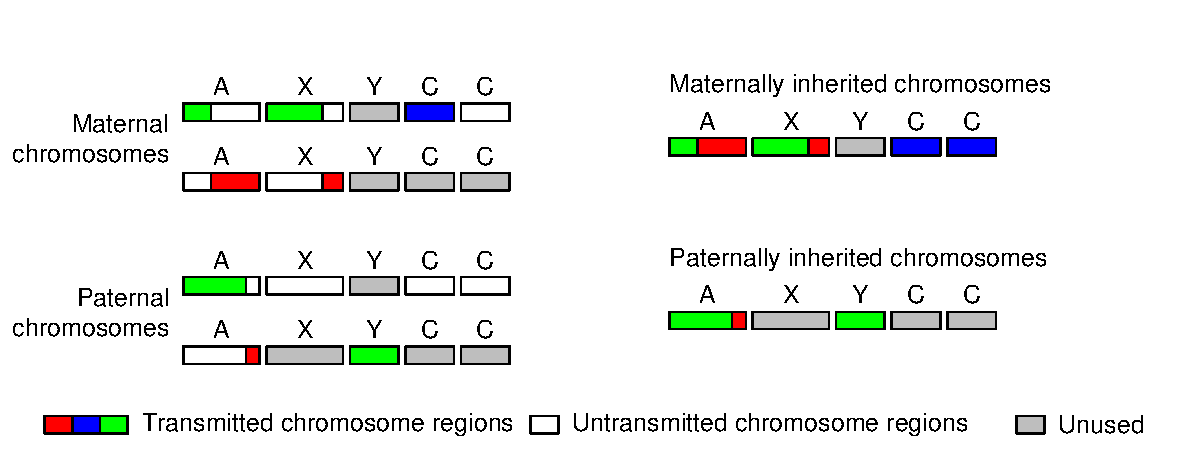
\includegraphics[width=0.9\textwidth]{figures/chromType}
\par\end{centering}
individuals in this population have five chromosomes, one autosome
(A), one X chromosome (X), one Y chromosome (Y) and two customized
chromosomes (C). The customized chromosomes model multiple copies
of mitochondrial chromosomes that are passed randomly from mother
to offspring. Y chromosomes for the female parent, the second copy
of chromosome X and the first copy of chromosome Y for the male parent,
and the second copy of customized chromosomes are unused (gray chromosome
regions). A male offspring inherits one copy of autosome from his
mother (with recombination), one copy of autosome from his father
(with recombination), an X chromosome from his mother (with recombination),
a Y chromosome from his father (without recombination), and two copies
of the first customized chromosome.
\end{figure}


\subsection{Information fields\label{subsec:stru-infoFields}}

Different kinds of simulations require different kinds of individuals.
individuals with only genotype information are sufficient to simulate
the basic Wright-Fisher model. Sex is needed to simulate such a model
in diploid populations with sex. individual fitness may be needed
if selection is induced, and age may be needed if the population is
age-structured. In addition, different types of quantitative traits
or affection status may be needed to study the impact of genotype
on Individual phenotype. Because it is infeasible to provide all such
information to an individual, simuPOP keeps genotype, sex (\texttt{MALE}
or \texttt{FEMALE}) and affection status as \emph{built-in properties}
of an individual, and all others as optional \emph{information fields}
(float numbers) attached to each individual.

Information fields can be specified when a population is created,
or added later using population member functions. They are essential
for proper operation of many simuPOP operators. For example, all selection
operators require information field \texttt{fitness} to store evaluated
fitness values for each individual. Operator \texttt{Migrator} uses
information field \texttt{migrate\_to} to store the ID of subpopulation
an individual will migrate to. An error will be raised if these operators
are applied to a population without needed information fields.

\lstinputlisting[caption={Basic usage of information fields},label={basicInfoFields}]{log/infoField.log}

Example \ref{basicInfoFields} demonstrates the basic usage of information
fields. In this example, a population with two information fields
\texttt{mother\_idx} and \texttt{father\_idx} are created. Besides
the present generation, this population keeps one ancestral generations
(\texttt{ancGen=1}, see Section \ref{subsec:Ancestral-populations}
for details). After initializing each individual with two chromosomes
with all zero and all one alleles respectively, the population evolves
one generation, subject to recombination at rate 0.01. Parents of
each individual are recorded, by operator \texttt{ParentsTagger},
to information fields \texttt{mother\_idx} and \texttt{father\_idx}
of each offspring\texttt{.}

After evolution, the population is extracted from the simulator, and
the values of information field \texttt{mother\_idx} of all individuals
are printed. The next several statements get the first Individual
from the population, and his mother from the parental generation using
the indexes stored in this individual's information fields. Genotypes
at the first homologous copy of this individual's chromosome is printed,
along with two parental chromosomes.

\textbf{Information fields can only be added or removed at the population
level} because all individuals need to have the same set of fields.
Values of information fields could be accessed at Individual or population
levels, using functions such as \texttt{Individual.info}, \texttt{Individual.setInfo},
\texttt{population.indInfo}, \texttt{Population.setIndInfo}. These
functions will be introduced in their respective classes.
\begin{note}
Information fields can be located both by names and by indexes\textbf{,}
the former provides better readability at a slight cost of performance
because these names have to be translated into indexes each time.
However, use of names are recommended in most cases for readability
considerations.
\end{note}

\section{Individual}

individuals are building blocks of a population. An individual object
cannot be created independently, but references to inidividuals can
be retrieved using member functions of a population object.

\subsection{Access individual genotype }

From a user's point of view, genotypes of an individual are stored
sequentially and can be accessed locus by locus, or in batch. The
alleles are arranged by position, chromosome and ploidy. That is to
say, the first allele on the first chromosome of the first homologous
set is followed by alleles at other loci on the same chromosome, then
markers on the second and later chromosomes, followed by alleles on
the second homologous set of the chromosomes for a diploid individual.
A consequence of this memory layout is that alleles at the same locus
of a non-haploid individual are separated by \texttt{Individual.totNumLoci()}
loci. The memory layout of a diploid individual with two chromosomes
is illustrated in Figure \ref{fig:genotype-layout}.

\begin{figure}[h]
\caption{\label{fig:genotype-layout}Memory layout of individual genotype}

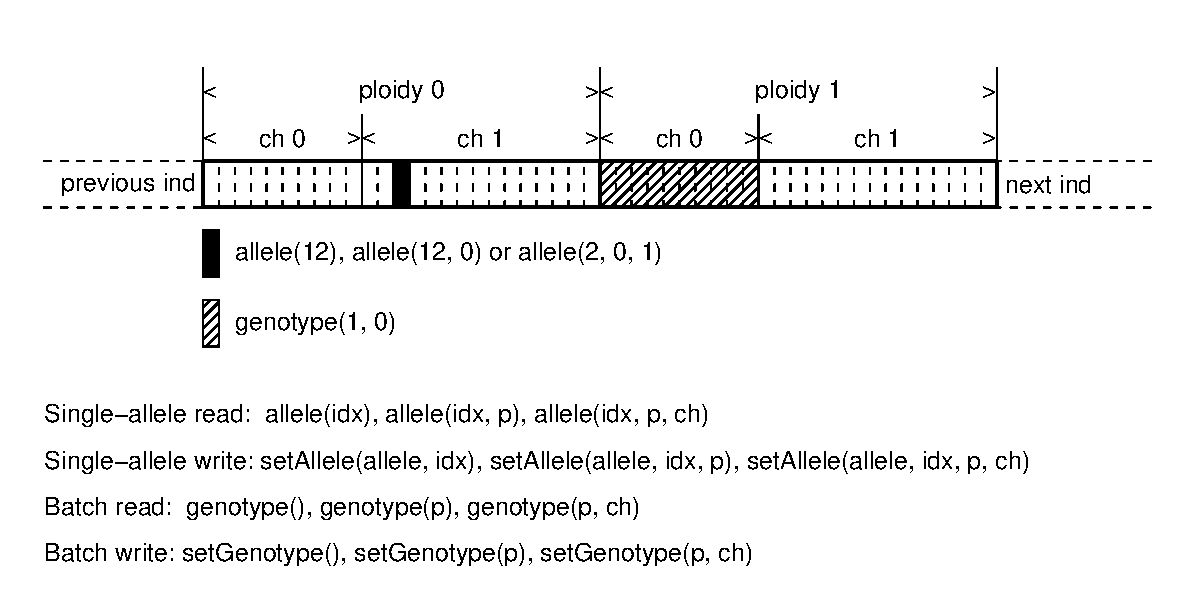
\includegraphics[width=0.9\textwidth]{figures/genotype}
\end{figure}

simuPOP provides several functions to read/write individual genotype.
For example, \texttt{Individual.allele()} and \texttt{Individual.setAllele()}
can be used to read and write single alleles. You could also access
alleles in batch mode using functions \texttt{Individual.genotype()}
and \texttt{Individual.setGenotype()}. It is worth noting that, instead
of copying genotypes of an individual to a Python tuple or list, the
return value of function \texttt{genotype({[}p, {[}ch{]}{]})} is a
special python carray object that reflects the underlying genotypes.
This object behaves like a regular Python list except that the underlying
genotype will be changed if elements of this object are changed. Only
\texttt{count(x)} and\texttt{ index(x, {[}start, {[}stop{]}{]})} member
functions can be used, but all comparison, assignment and slice operations
are allowed. If you would like to copy the content of this \texttt{carray}
to a Python list, use the \texttt{list()} function. Example \ref{individualGenotype}
demonstrates the use of these functions. \lstinputlisting[caption={Access individual genotype},label={individualGenotype}]{log/individualGenotype.log}

The same object will also be returned by function \texttt{Population.genotype()}.

\subsection{individual sex, affection status and information fields}

In addition to structural information shared by all individuals in
a population, the individual class provides member functions to get
and set \emph{genotype}, \emph{sex}, \emph{affection status} and \emph{information
fields} of an individual. Example \ref{individuals} demonstrates
how to access and modify individual sex, affection status and information
fields. Note that \textbf{information fields can be accessed as attributes
of individuals}. For example, \texttt{ind.info('father\_idx')} is
equivalent to \texttt{ind.father\_idx} and \texttt{ind.setInfo(35,
'age')} is equivalent to \texttt{ind.age = 35}.

\lstinputlisting[caption={Access Individual properties},label={individuals}]{log/individual.log}

\section{Population}

The \texttt{Population\index{Population}} object is the most important
object of simuPOP. It consists of one or more generations of individuals,
grouped by subpopulations, and a local Python dictionary to hold arbitrary
population information. This class provides a large number of functions
to access and modify population structure, individuals and their genotypes
and information fields. The following sections explain these features
in detail.

\subsection{Access and change individual genotype}

From a user's point of view, genotypes of all individuals in a population
are arranged sequentially. Similar to functions \texttt{Individual.genotype()}
and \texttt{Individual.setGenotype()}, genotypes of a population can
be accessed in batch using functions \texttt{Population.genotype()}
and \texttt{Population.setGenotype()}. However, because it is error
prone to locate an allele of a particular individual in this long
array, these functions are usually used to perform population-level
genotype operations such as clearing all alleles (e.g. \texttt{pop.setGenotype(0)})
or counting the number of a particular allele across all individuals
(e.g. \texttt{pop.genotype().count(1)}).

Another way to change alleles across the whole population is to recode
existing alleles to other numbers. This is sometimes needed if you
need to change allele states to conform with a particular mutation
model, assumptions of other software applications or genetic samples.
For example, if your dataset uses 1, 2, 3, 4 for A, C, T, G alleles,
and you would like to use alleles 0, 1, 2 and 3 for A, C, G, T (a
convention for simuPOP when nucleotide mutation models are involved),
you can use
\begin{lstlisting}
pop.recodeAlleles([0, 0, 1, 3, 2], alleleNames=['A', 'C', 'G', 'T'])
\end{lstlisting}
to convert and rename the alleles (1 allele to 0, 2 allele to 1, etc).
This operation will be applied to all subpopulations for all ancestral
generations, but can be restricted to selected loci.

\subsection{Subpopulations}

A simuPOP population consists of one or more subpopulations. \textbf{If
a population is not structured, it has one subpopulation that is the
population itself.} Subpopulations serve as barriers of individuals
in the sense that mating only happens between individuals in the same
subpopulation. A number of functions are provided to merge, remove,
resize subpopulations, and move individuals between subpopulations
(migration).

Example \ref{subPopName} demonstrates how to use some of the subpopulation
related functions. 

\lstinputlisting[caption={Manipulation of subpopulations},label={subPop}]{log/subPop.log}

Some population operations change the IDs of subpopulations. For example,
if a population has three subpopulations 0, 1, and 2, and subpopulation
1 is split into two subpouplations, subpopulation 2 will become subpopulation
3. Tracking the ID of a subpopulation can be problematic, especially
when conditional or random subpopulation operations are involved.
In this case, you can specify names to subpopulations. These names
will follow their associated subpopulations during population operations
so you can identify the ID of a subpopulation by its name. Note that
simuPOP allows duplicate subpopulation names.

\lstinputlisting[caption={Use of subpopulation names},label={subPopName}]{log/subPopName.log}


\subsection{Virtual subpopulations and virtual splitters {*}}

simuPOP subpopulations can be further divided into virtual subpopulations
(VSP), which are groups of individuals who share certain properties.
For example, all male individuals, all unaffected individuals, all
individuals with information field age > 20, all individuals with
genotype 0, 0 at a given locus, can form VSPs. VSPs do not have to
add up to the whole subpopulation, nor do they have to be non-overlapping.
Unlike subpopulations that have strict boundaries, VSPs change easily
with the changes of individual properties.

VSPs are defined by virtual splitters. \textbf{It is a definition
for groups of individuals in each subpopulation.} A splitter defines
the same number of VSPs in all subpopulations, although sizes of these
VSPs vary across subpopulations due to subpopulation differences.
For example, a \texttt{SexSplitter()} defines two VSPs, the first
with all male individuals and the second with all female individuals,
and a \texttt{InfoSplitter(field='x', values={[}1, 2, 4{]})} defines
three VSPs whose members have values \texttt{1}, \texttt{2} and \texttt{4}
at information field \texttt{x}, respectively. This splitter also
allows the use of cutoff values and ranges to define VSPs. If different
types of VSPs are needed, a combined splitter can be used to combine
VSPs defined by several splitters.

A VSP is represented by a \texttt{{[}sp, vsp{]}} pair where \texttt{sp}
and \texttt{vsp} can be subpopulation indexes or names. Its name and
size can be obtained using functions \texttt{subPopName()} and \texttt{subPopSize()}.
Example \ref{virtualSplitter} demonstrates how to apply virtual splitters
to a population, and how to check VSP names and sizes. \lstinputlisting[caption={Define virtual subpopulations in a population},label={virtualSplitter}]{log/virtualSplitter.log}

VSP provides an easy way to access groups of individuals in a subpopulation
and allows finer control of an evolutionary process. For example,
mating schemes can be applied to VSPs which makes it possible to apply
different mating schemes to, for example, individuals with different
ages. By applying migration, mutation etc to VSPs, it is easy to implement
advanced features such as sex-biased migrations, different mutation
rates for individuals at different stages of a disease. Example \ref{virtualSubPop}
demonstrates how to initialize genotype and information fields to
individuals in male and female VSPs. \lstinputlisting[caption={Applications of virtual subpopulations},label={virtualSubPop}]{log/virtualSubPop.log}

\subsection{Advanced virtual subpopulation splitters {*}{*}}

simuPOP provides a number of virtual splitters that can define VSPs
using specified properties. For example, \texttt{InfoSplitter(field='a',
values={[}1,2,3{]})} defines three VSPs whose individuals have values
\texttt{1}, \texttt{2}, and \texttt{3} at information field \texttt{a},
respectively; \texttt{SexSplitter()} defines two VSPs of male and
female individuals, respectively; and \texttt{RangeSplitter(ranges={[}{[}0,
2000{]}, {[}2000, 5000{]}{]})} defines two VSPs using two blocks of
individuals.

A \texttt{CombinedSplitter} can be used if your simulation needs more
than one sets of VSPs. For example, you may want to split your subpopulations
both by sex and by affection status. In this case, you can define
a combined splitter using 
\begin{lstlisting}
CombinedSplitter(splitters=[SexSplitter(), AffectionSplitter()])
\end{lstlisting}
This splitter simply stacks VSPs defined in \texttt{AffectionSplitter()}
after \texttt{SexSplitter()} so that unaffected and affected VSPs
are now VSPs 2 and 3 (0 and 1 are used for male and female VSPs).

There are also scenarios when you would like to define finer VSPs
with individuals belonging to more than one VSPs. For example, you
may want to have a look of frequencies of certain alleles in affected
male vs affected females, or count the number of males and females
with certain value at an information field. In this case, a \texttt{ProductSplitter}
can be used to define VSPs using interactions of several VSPs. For
example,
\begin{lstlisting}
ProductSplitter(splitters=[SexSplitter(), AffectionSplitter()])
\end{lstlisting}
defines 4 subpopulations by splitting VSPs defined by \texttt{SexSplitter()}
with affection status. These four VSPs will then have unaffected male,
affected male, unaffected female and affected female individuals,
respectively.

If you consider \texttt{ProductSplitter} as an intersection splitter
that defines new VSPs as intersections of existing VSPs, you may wonder
how to define unions of VSPs. For example, you can make a case where
you want to consider Individuals with information field a < 0 or a
> 100 together. A regular \texttt{InfoSplitter(field='a', cutoff={[}0,
100{]})} cannot do that because it defines three VSPs with $a<0$,
$0\leq a<100$ and $a\geq100$, respectively. The trick here is to
use parameter \texttt{vspMap} of a \texttt{CombinedSplitter}. If this
parameter is defined, multiple VSPs could be groups or reordered to
define a new set of VSPs. For example, 
\begin{lstlisting}
CombinedSplitter(splitters=[InfoSplitter(field='a', cutoff=[0, 100])], vspMap=[[0,2], 1])
\end{lstlisting}
 defines two VSPs using VSPs 0 and 2, and VSP 1 defined by the \texttt{InfoSplitter}
so that the first VSP contains individuals with $a<0$ or $a\geq100$.

Example \ref{advancedVSP} demonstrates some advanced usages of virtual
splitters.\lstinputlisting[caption={Advanced virtual subpopulation usages.},label={advancedVSP}]{log/advancedVSP.log}

\subsection{\label{subsec:Individuals}Access individuals and their properties}

There are many ways to access individuals of a population. For example,
function \texttt{Population.Individual(idx)} returns a reference to
the \texttt{idx}-th individual in a population. An optional parameter
\texttt{subPop} can be specified to return the \texttt{idx}-th individual
in the \texttt{subPop}-th subpopulation.

If you would like to access a group of individuals, either from a
whole population, a subpopulation, or from a virtual subpopulation,
\texttt{Population.individuals({[}subPop{]})} is easier to use. This
function returns a Python iterator that can be used to iterate through
individuals. An advantage of this function is that \texttt{subPop
}can be a virtual subpopulation which makes it easy to iterate through
Individuals with certain properties (such as all male Individuals).
If you would like to iterate through multiple virtual subpopulations
in one or more ancestral generations, you can use another function
\texttt{Population.allIndividuals(subPops, ancGens)}.

If more than one generations are stored in a population, function
\texttt{ancestor(idx, {[}subPop{]}, gen)} can be used to access Individual
from an ancestral generation (see Section \ref{subsec:Ancestral-populations}
for details). Because there is no group access function for ancestors,
it may be more convenient to use \texttt{useAncestralGen} to make
an \emph{ancestral} generation the \emph{current} generation, and
use \texttt{Population.Individuals}. Note that ancestor() function
can always access individuals at a certain generation, regardless
which generation the current generation is. Example \ref{batchAccess}
demonstrates how to use all these Individual-access functions.

If an unique ID is assigned to all individuals in a population, you
can look up individuals from their IDs using function \texttt{Population.indByID()}.
The information field to save individual ID is usually \texttt{ind\_id}
and you can use operator \texttt{IdTagger} and its function form \texttt{tagID}
to set this field. Note that this function can be used to look up
individuals in the present and all ancestral generations, although
a parameter (\texttt{ancGen}) can be used to limit search to a specific
generation if you know in advance which generation the individual
locates.

\lstinputlisting[caption={Access individuals of a population},label={accessIndividual}]{log/accessIndividual.log}

Although it is easy to access individuals in a population, it is often
more efficient to access genotypes and information fields in batch
mode. For example, functions \texttt{genotype()} and\texttt{ setGenotype()}
can read/write genotype of all individuals in a population or (virtual)
subpopulation, functions \texttt{indInfo()} and \texttt{setIndInfo()}
can read/write certain information fields in a population or (virtual)
subpopulation. The write functions work in a circular manner in the
sense that provided values are reused if they are not enough to fill
all genotypes or information fields. Example \ref{batchAccess} demonstrates
the use of such functions.

\lstinputlisting[caption={Access Individual properties in batch mode},label={batchAccess}]{log/batchAccess.log}

\subsection{Attach arbitrary auxillary information using information fields\label{sec:Information-fields}}

Information fields are usually set during population creation, using
the \texttt{infoFields} parameter of the population constructor. It
can also be set or added using functions \texttt{setInfoFields, addInfoField
}and \texttt{addInfoFields}. Example \ref{popInfo} demonstrates how
to read and write information fields from an individual, or from a
population in batch mode. Note that functions \texttt{Population.indInfo}
and \texttt{Population.setIndInfo} can be applied to (virtual) subpopulation
using a optional parameter subPop.

\lstinputlisting[caption={Add and use of information fields in a population},label={popInfo}]{log/popInfo.log}

\subsection{\label{subsec:Ancestral-populations}Keep track of ancestral generations}

A simuPOP population usually holds individuals in one generation.
During evolution, an offspring generation will replace the parental
generation and become the present generation (population), after it
is populated from a parental population. The parental generation is
discarded.

This is usually enough when only the present generation is of interest.
However, parental generations can provide useful information on how
genotype and other information are passed from parental to offspring
generations. simuPOP provides a mechanism to store and access arbitrary
number of ancestral generations in a population object. Applications
of this feature include pedigree tracking, reconstruction, and pedigree
ascertainments.

A parameter \texttt{ancGen} is used to specify how many generations
a population object \emph{can} store (which is usually called the
\emph{ancestral depth} of a population). This parameter is default
to \texttt{0}, meaning keeping no ancestral population. You can specify
a positive number \texttt{n} to store n most recent generations; or
-\texttt{1} to store all generations. Of course, storing all generations
during an evolutionary process is likely to exhaust the RAM of your
computer quickly.

Several member functions can be used to manipulate ancestral generations:
\begin{itemize}
\item \texttt{ancestralGens() }returns the number of ancestral generations
stored in a population.
\item \texttt{setAncestralDepth(depth)} resets the number of generations
a population can store.
\item \texttt{push(pop)} will push population \texttt{pop} into the current
population. \texttt{pop} will become the current generation, and the
current generation will either be removed (if ancGen == 0), or become
the parental generation of pop. The greatest ancestral generation
may be removed. This function is rarely used because populations with
ancestral generations are usually created during an evolutionary process.
\item \texttt{useAncestralGen(idx)} set the present generation to \texttt{idx}
generation. \texttt{idx} \texttt{= 1} for the parental generation,
\texttt{2} for grand-parental, ..., and \texttt{0} for the present
generation. This is useful because most population functions act on
the \emph{present} generation. You should always call \texttt{setAncestralPop(0)}
after you examined the ancestral generations. 
\end{itemize}
If a population has several ancestral generations, they are referred
by their indexes 0 (the latest generation), 1 (parental generation),
... and $k$ (top-most ancestral generation) where $k$ equals to
\texttt{ancestralGens()}. In many cases, you can retrieve the properties
of ancestral generations directly, using functions such as
\begin{itemize}
\item \texttt{popSize(ancGen=-1), subPopSizes(ancGen=-1), subPopSize(subPop,
ancGen=-1)}: population and subpopulation sizes of ancestral generation
\texttt{ancGen}.
\item \texttt{ancestor(index, ancGen)}: Get a reference to the \texttt{index}
individual of ancestral generation \texttt{ancGen}.
\end{itemize}
However, most population member functions work at the current generation
so you will need to switch to an ancestral generation using function
\texttt{useAncestralGen()} if you would like to manipulate an ancestral
generation. For example, you can remove the second subpopulation of
the parental generation using functions:
\begin{lstlisting}
pop.useAncestralGen(1)
pop.removeSubPops(1)
\end{lstlisting}

A typical use of ancestral generations is demonstrated in example
\ref{extract}. In this example, a population is created and is initialized
with allele frequency 0.5. Its ancestral depth is set to 2 at the
beginning of generation 18 so that it can hold parental generations
at generation 18 and 19. The allele frequency at each generation is
calculated and displayed, both during evolution using a \texttt{Stat}
operator, and after evolution using the function form this operator.
Note that setting the ancestral depth at the end of an evolutionary
process is a common practice because we are usually only interested
in the last few generations.

\lstinputlisting[caption={Ancestral populations},label={ancestralPop}]{log/ancestralPop.log}

\subsection{Change genotypic structure of a population }

Several functions are provided to remove, add empty loci or chromosomes,
and to merge loci or chromosomes from another population. They can
be used to trim unneeded loci, expand existing population or merge
two populations. Example \ref{extract} demonstrates how to use these
populations. Note that function \texttt{Population.addLociFrom} by
default merges chromosomes one by one according to chromosome index.
If \texttt{byName} is set to True, it will try to match chromosomes
by name and merge them. This example also demonstrates the use of
\texttt{DBG\_WARNING} flag, which will trigger a warning message when
chromosomes with different names are merged. \lstinputlisting[keywordstyle={\ttfamily},caption={Add and remove loci and chromosomes},label={addRemoveLoci}]{log/addRemoveLoci.log}

\subsection{Remove or extract individuals and subpopulations from a population}

Functions \texttt{Population.removeIndividuals} and \texttt{Population.removeSubPops}
remove selected individuals or groups of individuals from a population.
Functions \texttt{Population.extractIndividuals} and \texttt{Population.extractSubPops}
extract individuals and subpopulations from an existing population
and form a new one.

Functions \texttt{removeIndividauls} and \texttt{extractIndividuals}
could be used to remove or extract individuals from the present generation
by indexes or from all ancestral generations by IDs or a Python filter
function. This function should accept parameter \texttt{ind} or one
or more information fields. simuPOP will pass individual for parameter
\texttt{ind}, and values at specified information fields (\texttt{age}
in this example) of each individual to this function. The present
population structure will be kept, even if some subpopulations are
left empty. For example, you could remove the first thirty individuals
of a population using 
\begin{lstlisting}
pop.removeIndividuals(indexes=range(30))
\end{lstlisting}
or remove all individuals at age 20 or 30 using 
\begin{lstlisting}
pop.removeIndividuals(IDs=(20, 30), idField='age')
\end{lstlisting}
or remove all individuals with age between 20 and 30 using 
\begin{lstlisting}
pop.removeIndividuals(filter=lambda age: age >=20 and age <=30)
\end{lstlisting}
. In the last example, a Python lambda function is defined to avoid
the definition of a named function.

Functions \texttt{removeSubPops} or \texttt{extractSubPops} could
be used to remove or extract subpopulations, or goups of individuals
defined by virtual subpopulations from a population. The latter case
is very interesting because it could be used to remove or extract
individuals with similar properties, such as all individuals between
the ages 40 and 60, as demonstrated in Example \ref{extract}.

\lstinputlisting[loci and information fields from an existing population},keywordstyle={\ttfamily},caption={Extract individuals,label={extract}]{log/extract.log}

\subsection{\label{subsec:Population-Variables}Store arbitrary population information
as population variables}

Each simuPOP population has a Python dictionary that can be used to
store arbitrary Python variables. These variables are usually used
by various operators to share information between them. For example,
the \texttt{Stat\index{operator!Stat}} operator calculates population
statistics and stores the results in this Python dictionary. Other
operators such as the \texttt{PyEval} and \texttt{TerminateIf }read
from this dictionary and act upon its information.

simuPOP provides two functions, namely \texttt{Population.vars\index{Population!vars}()}
and \texttt{Population.\index{Population!Population}dvars()} to access
a population dictionary. These functions return the same dictionary
object but \texttt{dvars()} returns a wrapper class so that you can
access this dictionary as attributes. For example, \texttt{pop.vars(){[}'alleleFreq'{]}{[}0{]}}
is equivalent to \texttt{pop.dvars().alleleFreq{[}0{]}}. Because dictionary
\texttt{subPop{[}spID{]}} is frequently used by operators to store
variables related to a particular (virtual) subpopulation, function
\texttt{pop.vars(subPop)} is provided as a shortcut to \texttt{pop.vars(){[}'subPop'{]}{[}spID{]}}.
Example \ref{popVars} demonstrates how to set and access population
variables.

\lstinputlisting[caption={population variables},label={popVars}]{log/popVars.log}

It is important to understand that this dictionary forms a \textbf{local
namespace} in which Python expressions can be evaluated. This is the
basis of how expression-based operators work. For example, the \texttt{PyEval
}operator in example \ref{simple-example} evaluates expression \texttt{``'\%.2f\textbackslash t'
\% LD{[}0{]}{[}1{]}''} in each population's local namespace when it
is applied to that population. This yields different results for different
population because their LD values are different. In addition to Python
expressions, Python statements can also be executed in the local namespace
of a population, using the \texttt{stmts} parameter of the \texttt{PyEval}
or \texttt{PyExec} operator. Example \ref{expression} demonstrates
the use of a simuPOP terminator, which terminates the evolution of
a population when its expression is evaluated as \texttt{True}. Note
that The \texttt{evolve() }function of this example does not specify
how many generations to evolve so it will stop only after all replicates
stop. The return value of this function indicates how many generations
each replicate has evolved. This example also demonstrates how to
run multiple replicates of an evolutionary process, which we will
discuss in detail latter.

\lstinputlisting[caption={Expression evaluation in the local namespace of a population},label={expression}]{log/expression.log}

\subsection{\label{subsec:Save-and-Load}Save and load a population}

simuPOP populations can be saved to and loaded from disk files using
\texttt{Population.save\index{Population!save}(file)} member function
and global function \texttt{loadPopulation}\index{function!loadPopulation}.
\textbf{Virtual splitters are not saved} because they are considered
as runtime definitions. Although files in any extension can be used,
extension \texttt{.pop} is recommended. Example \ref{savePop} demonstrates
how to save and load a population in the native simuPOP format. \lstinputlisting[caption={Save and load a population},label={savePop}]{log/savePop.log}

The native simuPOP format is portable across different platforms but
is not human readable and is not recognized by other applications.
If you need to save a simuPOP population in a format that is recognizable
by a particular software, you can use functions \texttt{importPopulation},
\texttt{export}, and operator \texttt{Exporter} if you would like
to export populations during evolution. These functions are defined
in module \texttt{simuPOP.utils}. 

\subsection{Import and export datasets in unsupported formats {*}}

simuPOP provides a few utility functions to import and export populations
in common formats such as GENEPOP, Phylip, and STRUCTURE (see chapter
utility modules for details). If you need to import data from a file
in a format that is not currently supported, you generally need to
first scan the file for information such as number and names of chromosomes,
loci, alleles, subpopulation, and individuals. After you create a
population without genotype information from these parameters, you
can scan the file for the second time and fill the population with
genotypes and other information. Example \ref{importData} demonstrates
how to define a function to import from a file that is saved by function
\texttt{utils.saveCSV}.

\lstinputlisting[caption={Import a population from another file format},label={importData}]{log/importData.log}

Unless there are specific requirements in the order and labeling of
individuals, exporting a simuPOP population is usually straightforward.
Functions that are useful in such occasions include structural functions
\texttt{Population.numSubPop()}, \texttt{Population.subPopName(),
Population.popSize()} and \texttt{Population.subPopSizes()}, \texttt{and}
individual access functions \texttt{Population.individual()} and \texttt{Population.individuals()}
and individual population access functions such as \texttt{Individual.allele()}
and \texttt{Individual.info()}. Function \texttt{saveFSTAT} in the
cookbook module \texttt{fstatUtil} or \texttt{saveCSV} in module \texttt{simuPOP.utils}
are good examples you can follow.

\chapter{simuPOP Operators\label{cha:simuPOP-Operators}}

simuPOP is large, consisting of more than 70 operators and various
functions that covers all important aspects of genetic studies. These
includes mutation (\emph{k}-allele, stepwise, generalized stepwise),
migration (arbitrary, can create new subpopulation), recombination
(uniform or nonuniform), gene conversion, quantitative trait, selection,
penetrance (single or multi-locus, hybrid), ascertainment (case-control,
affected sibpairs, random), statistics calculation (allele, genotype,
haplotype, heterozygote number and frequency; expected heterozygosity;
bi-allelic and multi-allelic $D$, $D'$ and $r^{2}$ linkage disequilibrium
measures; $F_{st}$, $F_{it}$ and $F_{is}$); pedigree tracing, visualization
(using R or other Python modules). This chapter covers the basic and
some not-so-basic usages of these operators, organized roughly by
genetic factors.

\section{Introduction to operators}

Operators are objects that act on populations. There are two types
of operators:
\begin{itemize}
\item \textbf{Operators that are applied to populations}. These operators
are used in the \texttt{initOps}, \texttt{preOps}, \texttt{postOps}
and \texttt{finalOps} parameters of the \texttt{evolve} function.
The \texttt{initOps} operators are applied before an evolutionary
process, the \texttt{preOps} operators are applied to the parental
population at each generation before mating, the \texttt{postOps}
operators are applied to the offspring population at each generation
after mating, and the \texttt{finalOps} operators are applied after
an evolutionary process. Examples of such operators include \texttt{MergeSubPops}
to merge subpopulations and \texttt{StepwiseMutator} to mutate individuals
using a stepwise mutation model.
\item \textbf{Operators that are applied to individuals} (offspring) during
mating. These operators are used in the \texttt{ops} parameter of
a mating scheme. They are usually used to transmit genotype or other
information from parents to offspring. Examples of such operators
include \texttt{MendelianGenoTransmitter} that transmit parental genotype
to offspring according to Mendelian laws and \texttt{ParentsTagger}
that record the indexes of parents in the parental population to each
offspring.
\end{itemize}
Some mutators could be applied both to populations and individuals.
For example, an \texttt{IdTagger} could be applied to a whole population
and assign an unique ID to all individuals, or to offspring during
mating.

The following sections will introduce common features of all operators.
The next chapter will explain all simuPOP operators in detail.

\subsection{Apply operators to selected replicates and (virtual) subpopulations
at selected generations}

Operators are, by default, applied to all generations during an evolutionary
process. This can be changed using the \texttt{begin}, \texttt{end},
\texttt{step} and \texttt{at} parameters. As their names indicate,
these parameters control the starting generation (\texttt{begin}),
ending generation (\texttt{end}), generations between two applicable
generations (\texttt{step}), and an explicit list of applicable generations
(\texttt{at}, a single generation number is also acceptable). Other
parameters will be ignored if \texttt{at} is specified. It is worth
noting that, if an evolutionary process has a pre-sepcified ending
generation, negative generations numbers are allowed. They are counted
backward from the ending generation.

For example, if a simulator starts at generation \texttt{0}, and the
\texttt{evolve} function has parameter \texttt{gen=10}, the simulator
will stop at the \emph{beginning} of generation \texttt{10}. Generation
\texttt{-1} refers to generation \texttt{9}, and generation \texttt{-2}
refers to generation \texttt{8}, and so on. Example \ref{applicableGen}
demonstrates how to set applicable generations of an operator. In
this example, a population is initialized before evolution using an
\texttt{InitGenotype} operator. allele frequency at locus \texttt{0}
is calculated at generation \texttt{80}, \texttt{90}, but not \texttt{100}
because the evolution stops at the beginning of generation \texttt{100}.
A \texttt{PyEval} operator outputs generation number and allele frequency
at the end of generation \texttt{80} and \texttt{90}. Another \texttt{PyEval}
operator outputs similar information at generation \texttt{90} and
\texttt{99}, before and after mating. Note, however, because allele
frequencies are only calculated twice, the pre-mating allele frequency
at generation \texttt{90} is actually calculated at generation \texttt{80},
and the allele frequencies display for generation \texttt{99} are
calculated at generation \texttt{90}. At the end of the evolution,
the population is saved to a file using a \texttt{SavePopulation}
operator. \lstinputlisting[caption={Applicable generations of an operator.},label={applicableGen}]{log/applicableGen.log}

\subsection{Applicable populations and (virtual) subpopulations}

A simulator can evolve multiple replicates of a population simultaneously.
Different operators can be applied to different replicates of this
population. This allows side by side comparison between simulations.

Parameter \texttt{reps} is used to control which replicate(s) an operator
can be applied to. This parameter can be a list of replicate numbers
or a single replicate number. Negative index is allowed where \texttt{-1}
refers to the last replicate. This technique has been widely used
to produce table-like output where a \texttt{PyOutput} outputs a newline
when it is applied to the last replicate of a simulator. Example \ref{hybridOperator}
demonstrates how to use this \texttt{reps} parameter. It is worth
noting that negative indexes are \emph{dynamic} indexes relative to
number of active populations. For example, \texttt{rep=-1} will refer
to a previous population if the last population has stopped evolving.
Use a non-negative replicate number if this is not intended. \lstinputlisting[caption={Apply operators to a subset of populations},label={replicate}]{log/replicate.log}

An operator can also be applied to specified (virtual) subpopulations.
For example, an \texttt{initializer} can be applied to male individuals
in the first subpopulation, and everyone in the second subpopulation
using parameter \texttt{subPops={[}(0,0)}, 1{]}, if a virtual subpopulation
is defined by individual sex. Generally speaking,
\begin{itemize}
\item \texttt{subPops={[}{]}} applies the operator to all subpopulation.
This is usually the default value of an operator.
\item \texttt{subPops={[}vsp1, vsp2,...{]}} applies the operator all specified
(virtual) subpopulations. (e.g. \texttt{subPops={[}(0,0)}, 1{]}).
\item \texttt{subPops=sp} is an abbreviation for \texttt{subPops={[}sp{]}}.
If \texttt{sp} is virtual, it has to be written as \texttt{{[}sp{]}}
because \texttt{subPops=(0, 1)} is intepreted as two non-virtual subpopulation.
\end{itemize}
However, not all operators support this parameter, and even if they
do, their interpretations of parameter input may vary. Please refer
to documentation for individual operators in \emph{the simuPOP reference
manual} for details.

\subsection{Dynamically determined loci (parameter \texttt{loci}) {*}}

Many operators accept a parameter \texttt{loci} to specify the applicable
loci. This parameter can be
\begin{itemize}
\item \texttt{ALL\_AVAIL}: all available loci of the population to which
the operator is applied.
\item {[}1, 2, 4, 5{]}: A list of loci indexes. When the operator is applied
to a population, it will be applied to the specified loci.
\item \texttt{{[}('chr1', 5), ('chr1', 10), ('chr2', 5){]}}: A list of chromosome
position pairs. That is to say, when the operator is applied to a
population, it will find loci at specified position of specified chromosome.
Here chromosome names are names specified by parameter \texttt{chromNames}
of the \texttt{Population} constructor. That is to say, the operator
can be applied to all population with such chromosomes and loci at
specified locations.
\item func: A function with an optional parameter \texttt{pop}. When the
operator is applied to a population, it will call this function, optionally
pass the population to be applied to this function, and use its output
as indexes of loci.
\end{itemize}
The last usage is very interesting because it allows the determination
of loci according to population property. For example, Example \ref{dynamicLoci}
shows an example with a \texttt{MaSelector} that is applied to the
locus with highest frequency at each generation by calling function
\texttt{mostPopular}, which calculates allele frequency and pick the
locus with highest allele frequency, This example looks silly, but
the technique is very useful in simulating the introduction of disease
loci by, for example, adding positive selection pressure to one of
the chosen loci. \lstinputlisting[caption={Natural selection with dynamically determined loci},label={dynamicLoci}]{log/dynamicLoci.log}

\subsection{Write output of operators to one or more files}

All operators we have seen, except for the \texttt{SavePopulation}
operator in Example \ref{applicableGen}, write their output to the
standard output, namely your terminal window. However, it would be
much easier for bookkeeping and further analysis if these output can
be redirected to disk files. Parameter \texttt{output} is designed
for this purpose.

Parameter \texttt{output} can take the following values:
\begin{itemize}
\item \texttt{''} (an empty string): No output.
\item \texttt{'>'}: Write to standard output.
\item \texttt{'filename'} or \texttt{'>filename'}: Write the output to a
file named filename. If multiple operators write to the same file,
or if the same operator writes to the file file several times, only
the last write operation will succeed.
\item \texttt{'>\textcompwordmark >filename'}: Append the output to a file
named filename. The file will be opened at the beginning of \texttt{evolve}
function and closed at the end. An existing file will be cleared.
\item \texttt{'>\textcompwordmark >\textcompwordmark >filename'}: This
is similar to the \texttt{'>\textcompwordmark >'} form but the file
will not be cleared at the beginning of the \texttt{evolve} function.
\item \texttt{'!expr'}: \texttt{expr} is considered as a Python expression
that will be evaluated at a population's local namespace whenever
an output string is needed. For example, \texttt{'!''\%d.txt'' \%
gen'} would return \texttt{0.txt}, \texttt{1.txt} etc at generation
\texttt{0}, \texttt{1}, ....
\item File handle of an opened file. Actually any python object with a \texttt{write}
function.
\item A Python function that can accept a string as its only parameter (\texttt{func(msg)}).
When an operator outputs a message, this function will be called with
this message.
\item A \texttt{WithMode(output, 'b')} object with \texttt{output} being
the any of the allowed output string or function. This object tells
simuPOP that the output is opened in binary model so that it should
output bytes instead of texts to it. This is mostly designed for Python
3 because file objects in Python 2 accepts string even if they are
opened in binary mode. 
\end{itemize}
Because a table output such as the one in Example \ref{hybridOperator}
is written by several operators, it is clear that all of them need
to use the \texttt{'>\textcompwordmark >'} output format.

The \texttt{SavePopulation} operator in Example \ref{applicableGen}
write to file \texttt{sample.pop}. This works well if there is only
one replicate but not so when the operator is applied to multiple
populations. Only the last population will be saved successfully!
In this case, the expression form of parameter \texttt{output} should
be used.

The expression form of this parameter accepts a Python expression.
Whenever a filename is needed, this expression is evaluated against
the local namespace of the population it is applied to. Because the
\texttt{evolve} function automatically sets variables \texttt{gen}
and \texttt{rep} in a population's local namespace, such information
can be used to produce an output string. Of course, any variable in
this namespace can be used so you are not limited to these two variable.

Example \ref{hybridOperator} demonstrates the use of these two parameters.
In this example, a table is written to file \texttt{LD.txt} using
\texttt{output='>\textcompwordmark >LD.txt'}. Similar operation to
\texttt{output='R2.txt'} fails because only the last $R^{2}$ value
is written to this file. The last operator writes output for each
replicate to their respective output file such as \texttt{LD\_0.txt},
using an expression that involves variable \texttt{rep}.\lstinputlisting[caption={Use the output and outputExpr parameters},label={output}]{log/output.log}

Example \ref{outputFunc} demonstrates an advanced usage of the \texttt{output}
parameter. In this example, a logging object is created to write to
a logfile as well as the standard output. The \texttt{info} and \texttt{debug}
functions of this object are assigned to two operators so that their
outputs can be sent to both a logfile and to the console window. One
of the advantages of using a logging mechanism is that debugging output
could be suppressed easily by adjusting the logging level of the logging
object. Note that function \texttt{logging.info()} automatically adds
a new line to its input messages before it writes them to an output.
\lstinputlisting[caption={Output to a Python function},label={outputFunc}]{log/outputFunc.log}

\subsection{During-mating operators}

All operators in Examples \ref{applicableGen}, \ref{replicate} and
\ref{output} are applied before or after mating. There is, however,
a hidden during-mating operator that is called by \texttt{RandomMating()}.
This operator is called \texttt{MendelianGenoTransmitter()} and is
responsible for transmitting genotype from parents to offspring according
to Mendel's laws. All pre-defined mating schemes (see Section \ref{sec:Mating-Schemes})
use a special kind of during-mating operator to transmit genotypes.
They are called \textbf{genotype transmitters} just to show the kind
of task they perform. More during mating operators could be specified
by replacing the default operator used in the \texttt{ops} parameter
of a mating scheme (or an offspring generator if you are defining
your own mating scheme).

Operators used in a mating scheme honor applicability parameters \texttt{begin},
\texttt{step}, \texttt{end}, \texttt{at} and \texttt{reps} although
they do not support negative population and replicate indexes. It
is therefore possible to apply different during-mating operators at
different generations. For example, a \texttt{Recombinator} is used
in Example \ref{transmitter} to transmit parental genotypes to offspring
after generation 30 while the \texttt{MendelianGenoTransmitter} is
applied before that.

\lstinputlisting[caption={Genotype transmitters},label={transmitter}]{log/transmitter.log}

During-mating operators can be applied to (virtual) subpopulations
using parameter \texttt{subPops}, which \textbf{refers to (virtual)
subpopulations in the offspring population}. Section \ref{subsec:Pre-defined-genotype-transmitters}
and \ref{sec:Genotype-transmitters} list all genotype transmitters,
Section \ref{subsec:Customized-genotype-transmitter} demonstrates
how to define your own genotype transmitter, Section \ref{subsec:vspSelection}
demonstrates the use of during-mating operator in virtual subpopulations.

\subsection{Function form of an operator\label{subsec:Function-form}}

Operators are usually applied to populations through a simulator but
they can also be applied to a population directly. For example, it
is possible to create an \texttt{InitGenotype} operator and apply
to a population as follows:

\begin{lstlisting}
InitGenotype(freq=[.3, .2, .5]).apply(pop)
\end{lstlisting}
Similarly, you can apply the hybrid penetrance model defined in Example
\ref{hybridOperator} to a population by

\begin{lstlisting}
PyPenetrance(func=myPenetrance, loci=[10, 30, 50]).apply(pop)
\end{lstlisting}

This usage is used so often that it deserves some simplification.
Equivalent functions are defined for most operators. For example,
function \texttt{initGenotype} is defined for operator \texttt{InitGenotype}
as follows

\lstinputlisting[caption={The function form of operator \texttt{InitGenotype}},label={funcform}]{log/funcform.log}

These functions are called function form of operators. Using these
functions, the above two example can be written as 

\begin{lstlisting}
initGenotype(pop, freq=[.3, .2, .5])
\end{lstlisting}
and 

\begin{lstlisting}
pyPenetrance(pop, func=myPenetrance, loci=[10, 30, 50])
\end{lstlisting}
respectively. Note that applicability parameters such as \texttt{begin}
and \texttt{end} can still be passed, but they are ignored by these
functions.

Finally, it is worth noting that, if you have a function that manipulates
population, you can make it an operator by wrapping it in a \texttt{PyOperator}
so that it can be called repeatedly during evolution. For example,
for a function \texttt{myFunc} that works on a population, you can
define a wrapper function

\begin{lstlisting}
def Func(pop):
    # call myFunc
    myFunc(pop)
    return True
\end{lstlisting}

which can then use it in a \texttt{PyOperator} as follows:

\begin{lstlisting}
PyOperator(func=Func)
\end{lstlisting}

The wrapper function is not needed if myFunc returns \texttt{True}
by itself. It can also be simplifed to a lambda function

\begin{lstlisting}
PyOperator(func=lambda pop: myFunc(pop) is None)
\end{lstlisting}
if you are certain that \texttt{myFunc} does not return any value
(return \texttt{None}).
\begin{note}
Whereas output files specified by \texttt{'>'} are closed immediately
after they are written, those specified by \texttt{'>\textcompwordmark >'}
and \texttt{'>\textcompwordmark >\textcompwordmark >'} are not closed
after the operator is applied to a population. This is not a problem
when operators are used in a simulator because \texttt{Simulator.evolve}
closes all files opened by operators, but can cause trouble when the
operator is applied directly to a population. For example, multiple
calls to \texttt{dump(pop, output='>\textcompwordmark >file')} will
dump pop to \texttt{file} repeatedly but \texttt{file} will not be
closed afterward. In this case, \texttt{closeOutput('file')} should
be used to explicitly close the file.
\end{note}

\section{Initialization}

simuPOP provides three operators to initialize individual sex, information
fields and genotype at the population level. A number of parameter
are provided to cover most commonly used initialization scenarios.
A Python operator can be used to intialize a population explicitly
if none of the operators fits your need.

\subsection{Initialize individual sex (operator \texttt{InitSex})}

Operator \texttt{InitSex()} and function \texttt{initSex()} initialize
individual sex either randomly or using a given sequence. In the first
case, individuals are assigned \texttt{MALE} or \texttt{FEMALE} with
equal probability unless parameter \emph{maleFreq} is used to specify
the probability of having a male Individual. Alternatively, parameter
\emph{maleProp} can be used to specify exact proportions of male individuals
so that you will have exactly 1000 males and 1000 females if you apply
\texttt{InitSex(maleProp=0.5)} to a population of 2000 individuals.

Both parameters \texttt{maleFreq} and \texttt{maleProp} assigns individual
sex randomly. If for some reason you need to specify individual sex
explicitly, you could use a sequence of sex (\texttt{MALE} or \texttt{FEMALE})
to assign sex to individuals succesively. The list will be reused
if needed. If a list of (virtual) subpopulations are given, this operator
will only initialize individuals in these (virtual) subpopulations.
Example \ref{InitSex} demonstrates how to use two \texttt{InitSex}
operators to initialize two subpopulations. \lstinputlisting[caption={Initialize individual sex},label={InitSex}]{log/InitSex.log}

\subsection{Initialize genotype (operator \texttt{InitGenotype})}

Operator \texttt{InitGenotype} (and its function form \texttt{initGenotype})
initializes individual genotype by allele frequency, allele proportion,
haplotype frequency, haplotype proportions or a list of genotypes:
\begin{itemize}
\item By frequency of alleles. For example, \texttt{InitGenotype(freq=(0,
0.2, 0.4, 0.2))} will assign allele 0, 1, 2, and 3 with probability
0, 0.2, 0.4 and 0.2 respectively.
\item By proportions of alleles. For example, \texttt{InitGenotype(prop=(0,
0.2, 0.4, 0.2))} will assign 400 allele 1, 800 allele 2 and 400 allele
3 to a diploid population with 800 individuals.
\item By frequency of haplotypes. For example, \texttt{InitGenotype(haplotypes={[}{[}0,
0{]}, {[}1,1{]}, {[}0,1{]},{[}1,1{]}{]})} will assign four haplotypes
with equal probabilities. \texttt{InitGenotype(haplotypes={[}{[}0,
0{]}, {[}1,1{]}, {[}0,1{]},{[}1,1{]}{]}, freq={[}0.2, 0.2, 0.3, 0.3{]})}
will assign these haplotypes with different frequencies. If there
are more than two loci, the haplotypes will be repeated.
\item By frequency of haplotypes. For example, \texttt{InitGenotype(haplotypes={[}{[}0,
0{]}, {[}1,1{]}, {[}0,1{]},{[}1,1{]}{]}, prop={[}0.2, 0.2, 0.3, 0.3{]})}
will assign four haplotypes with exact proportions. 
\item By a list of genotype. For example, \texttt{InitGenotype(genotype={[}1,
2, 2, 1{]})} will assign genotype \texttt{1}, \texttt{2}, \texttt{2},
\texttt{1} repeatedly to a population. If individuals in this population
has two homologous copies of a chromosome with two loci, this operator
will assign haplotype \texttt{1}, \texttt{2} to the first homologous
copy of the chromosome, and \texttt{2}, \texttt{1} to the second copy.
\item By multiple allele frequencies or proportions returned by a function
passed to parameter \texttt{freq} or \texttt{prop} (new in version
1.1.7). This function can accept parameters \texttt{loc}, \texttt{subPop}
or \texttt{vsp} and returns locus, subpopopulation or virtual subpopulation
specific allele frequencies. For example, if you would like to initialize
genotypes with random allele frequency, you can set \texttt{freq=lambda
: random.random()} so that a new frequency is drawn from an uniform
distribution for each new locus. Note that simuPOP expects the return
value of this function to be a list of frequencies for alleles 0,
1, ..., but treats a single return value \emph{x} as {[}\emph{x, 1-x}{]}
for simplicity.
\end{itemize}
Parameter \texttt{loci} and \texttt{ploidy} can be used to specify
a subset of loci and homologous sets of chromosomes to initialize,
and parameter \texttt{subPops} can be used to specify subsets of individuals
to initialize. Example \ref{InitGenotype} demonstrates how to use
these the \texttt{InitGenotype} operator, including examples on how
to define and use virtual subpopulations to initialize individual
genotype by sex or by proportion.

\lstinputlisting[caption={Initialize individual genotype},label={InitGenotype}]{log/InitGenotype.log}

\subsection{Initialize information fields (operator \texttt{InitInfo})}

Operator \texttt{InitInfo} and its function form \texttt{initInfo}
initialize one or more information fields of all individuals or Individuals
in selected (virtual) subpopulations using either a list of values
or a Python function. If a value or a list of value is given, it will
be used repeatedly to assign values of specified information fields
of all applicable individuals. For example, \texttt{initInfo(pop,
values=1, infoFields='x')} will assign value \texttt{1} to information
field \texttt{x} of all individuals, and 
\begin{lstlisting}
initInfo(pop, values=[1, 2, 3], infoFields='x', subPops=[(0,1)])
\end{lstlisting}
will assign values \texttt{1}, \texttt{2}, \texttt{3}, \texttt{1},
\texttt{2}, \texttt{3}... to information field \texttt{x} of individuals
in the second virtual subpopulation of subpopulation 0.

The \texttt{values} parameter also accepts a Python function. This
feature is usually used to assign random values to an information
field. For example, \texttt{values=random.random} would assign a random
value between 0 and 1. If a function takes parameters, a lambda function
can be used. For example, 
\begin{lstlisting}
initInfo(pop, lambda : random.randint(2, 5), infoFields=['x', 'y'])
\end{lstlisting}
 assigns random integers between 2 and 5 to information fields \texttt{x}
and \texttt{y} of all individuals in \emph{pop}. Example \ref{InitInfo}
demonstrates these usages.

\lstinputlisting[caption={initialize information fields},label={InitInfo}]{log/InitInfo.log}

\section{Expressions and statements}

\subsection{Output a Python string (operator \texttt{PyOutput})}

Operator \texttt{PyOutput} is a simple operator that prints a Python
string when it is applied to a population. It is commonly used to
print the progress of a simulation (e.g. \texttt{PyOutput('start migration\textbackslash n',
at=200)}) or output separators to beautify outputs from \texttt{PyEval}
outputs (e.g. \texttt{PyOutput('\textbackslash n', rep=-1)}.

\subsection{Execute Python statements (operator \texttt{PyExec})}

Operator \texttt{PyExec} executes Python statements in a population's
local namespace when it is applied to that population. This operator
is designed to execute short Python statements but multiple statements
separated by newline characters are allowed.

Example \ref{PyExec} uses two \texttt{PyExec} operators to create
and use a variable \texttt{traj} in each population's local namespace.
The first operator initialize this variable as an empty list. During
evolution, the frequency of allele 1 at locus 0 is calcuated (operator
\texttt{Stat}) and appended to this variable (operator \texttt{PyExec}).
The result is a trajectory of allele frequencies during evolution.
\lstinputlisting[caption={Execute Python statements during evolution},label={PyExec}]{log/PyExec.log}

\subsection{Evaluate and output Python expressions (operator \texttt{PyEval})}

Operator \texttt{PyEval} evaluate a given Python expression in a population's
local namespace and output its return value. This operator has been
widely used (e.g. Example \ref{simple-example}, \ref{ancestralPop},
\ref{applicableGen} and \ref{output}) to output statistics of populations
and report progress.

Two additional features of this operator may become handy from time
to time. First, an optional Python statements (parameter \emph{stmts})
can be specified which will be executed before the expression is evaluated.
Second, the population being applied can be exposed in its own namespace
as a variable (parameter \emph{exposePop}). This makes it possible
to access properties of a population other than its variables. Example
\ref{PyEval} demonstrates both features. In this example, two statements
are executed to count the number of unique parents in an offspring
population and save them as variables \texttt{numFather} and \texttt{numMother}.
The operator outputs these two variables alone with a generation number. 

\lstinputlisting[caption={Evaluate a expression and statements in a population's local namespace.},label={PyEval}]{log/PyEval.log}

Note that the function form of this operator (\texttt{pyEval}) returns
the result of the expression rather than writting it to an output.

\subsection{Expression and statement involving individual information fields
(operator \texttt{InfoEval} and \texttt{InfoExec}) {*}}

Operators \texttt{PyEval} and \texttt{PyExec} work at the population
level, using the local namespace of populations. Operator \texttt{InfoEval}
and \texttt{InfoExec}, on the contraray, work at the individual level,
using individual information fields (and population variables) as
variables. In this case, individual information fields are copied
to the population namespace one by one before expression or statements
are executed for each individual. Optionally, the individual object
can be exposed to these namespace using a user-specified name (parameter
\emph{exposeInd}). Individual information fields will be updated if
the value of these fields are changed.

Operator \texttt{InfoEval} evaluates an expression and outputs its
value. Operator \texttt{InfoExec} executes one or more statements
and does not produce any output. Operator \texttt{InfoEval} is usually
used to output individual information fields and properties in batch
mode. It is faster and sometimes easier to use than corresponding
for loop plus individual level operations. For example
\begin{itemize}
\item \texttt{InfoEval(r'{}''\%.2f\textbackslash t'' \% a')} outputs
the value of information field a for all individuals, separated by
tabs.
\item \texttt{InfoEval('ind.sexChar()', exposeInd='ind')} outputs the sex
of all individuals using an exposed individual object \texttt{ind}.
\item \texttt{InfoEval('a+b{*}{*}2')} outputs $a+b^{2}$ for information
fields $a$ and $b$ for all individuals.
\end{itemize}
Example \ref{InfoEval} demonstrates the use of this operator.

\lstinputlisting[caption={Evaluate expressions using individual information fields},label={InfoEval}]{log/InfoEval.log}

Operator \texttt{InfoExec} is usually used to set individual information
fields. For example
\begin{itemize}
\item \texttt{InfoExec('age += 1')} increases the age of all individuals
by one.
\item \texttt{InfoExec('risk = 2 if packPerYear > 10 else 1.5')} sets information
field \texttt{risk} to \texttt{2} if \texttt{packPerYear} is greater
than \texttt{10}, and \texttt{1.5} otherwise. Note that conditional
expression is only available for Python version 2.5 or later.
\item \texttt{InfoExec('a = b{*}c')} sets the value of information field
\texttt{a} to the product of \texttt{b} and \texttt{c}.
\end{itemize}
Example \ref{InfoExec} demonstrates the use of this operator, using
its function form \texttt{infoExec}.

\lstinputlisting[caption={Execute statements using individual information fields},label={InfoExec}]{log/InfoExec.log}

Note that a statement can also be specified for operator \texttt{InfoEval},
which will be executed before an expression is evaluated.

\subsection{Using functions in external modules in simuPOP expressions and statements}

All simuPOP expressions and statements are evaluated in a population's
local namespace, which is a dictionary with no access to external
modules. If you would like to use external modules (e.g. functions
from the \texttt{random} module), you will have to import them to
the namespace explicitly, using something like

\begin{lstlisting}
exec('import random', pop.vars(), pop.vars())
\end{lstlisting}
before you evolve the population. 

Example \ref{outputByInterval} demonstrates the application of this
technique. This example imports the \texttt{time} module in the population's
local namespace and set \texttt{init\_time} and \texttt{last\_time}
before evolution. During evolution, an\texttt{ IfElse} operator is
used to output the status of the simulation for every 5 seconds using
expression \texttt{time.time() - last\_time > 5}. \texttt{last\_time}
is reset using the \texttt{PyExec} operator. The evolution will last
20 seconds and be terminated by the Terminator with expression \texttt{time.time()
- init\_time > 20.}

\lstinputlisting[caption={Write the status of an evolutionary process every 10 seconds},label={outputByInterval}]{log/outputByInterval.log}

\section{Demographic changes}

A mating scheme controls the size of an offspring generation using
parameter \texttt{subPopSize}. This parameter has been described in
detail in section \ref{subsec:offspring-size}. In summary,
\begin{itemize}
\item The subpopulation sizes of the offspring generation will be the same
as the parental generation if subPopSize is not set.
\item The offspring generation will have a fixed size if \texttt{subPopSize}
is set to a number (no subpopulation) or a list of subpopulation sizes. 
\item The subpopulation sizes of an offspring generation will be determined
by the return value of a demographic function if \texttt{subPopSize}
is set to such a function (a function that returns subpopulation sizes
at each generation).
\end{itemize}
\begin{note}
Parameter \texttt{subPopSize} only controls subpopulation sizes of
an offspring generation immediately after it is generated. population
or subpopulation sizes could be changed by other operators.
\end{note}
During mating, a mating scheme goes through each parental subpopulation
and populates its corresponding offspring subpopulation. This implies
that
\begin{itemize}
\item Parental and offspring populations should have the same number of
subpopulations.
\item Mating happens strictly within each subpopulation.
\end{itemize}
This section will introduce several operators that allow you to move
dndividuals across the boundary of subpopulations (migration), and
change the number of subpopulations during evolution (split and merge).
Please refer to \ref{subsec:offspring-size} (control the size of
the offspring generation section of chapter mating scheme) for more
details. For more advanced demographic models, please refer to the
\texttt{simuPOP.demography} module.

\subsection{Migration (operator \texttt{Migrator})}

\subsubsection{Migration by probability}

Operator \texttt{Migrator} (and its function form \texttt{migrate})
migrates individuals from one subpopulation to another. The key parameters
are
\begin{itemize}
\item \emph{from} subpopulations (parameter \texttt{subPops}). A list of
subpopulations from which individuals migrate. Default to all subpopulations.
\item \emph{to} subpopulations (parameter \texttt{toSubPops}). A list of
subpopulations to which individuals migrate. Default to all subpopulations.
\textbf{A new subpopulation ID can be specified to create a new subpopulation
from migrants.}
\item A migration rate matrix (parameter \texttt{rate}). A $m$ by $n$
matrix ( a nested list in Python) that specifies migration rate from
each source to each destination subpopulation. That is to say, $\mbox{rate}{}_{i,j}$
specifies migration rate from $\mbox{subPops}_{i}$ to $\mbox{toSubPops}_{j}$.
Needless to say, $m$ and $n$ are determined by the number of \emph{from}
and \emph{to} subpopulations.
\end{itemize}
Example \ref{migrateByProb} demonstrate the use of a \texttt{Migrator}
to migrate individuals between three subpopulations. Note that 
\begin{itemize}
\item Operator \texttt{Migrator} relies on an information field \texttt{migrate\_to}
(configurable) to record destination subpopulation of each individual
so this information field needs to be added to a population befor
migration.
\item Migration rates to subpopulation themselves are determined automatically
so they can be left unspecified.
\end{itemize}
\lstinputlisting[caption={Migration by probability},label={migrateByProb}]{log/migrateByProb.log}

\subsubsection{Migration by proportion and counts}

Migration rate specified in the rate parameter in Example \ref{migrateByProb}
is intepreted as probabilities. That is to say, a migration rate $r_{m,n}$
is interpreted as the probability at which any individual in subpopulation
$m$ migrates to subpopulation $n$. The exact number of migrants
are randomly distributed.

If you would like to specify exactly how many migrants migrate from
a subpopulation to another, you can specify parameter \texttt{mode}
of operator \texttt{Migrator} to \texttt{BY\_PROPORTION} or \texttt{BY\_COUNTS}.
The \texttt{BY\_PROPORTION} mode interpret $r_{m,n}$ as proportion
of individuals who will migrate from subpopulation $m$ to $n$ so
the number of $m\rightarrow n$ migrant will be exactly $r_{m,n}\times$subPopSize(m).
In the \texttt{BY\_COUNTS} mode, $r_{m,n}$ is interpretted as number
of migrants, regardless the size of subpopulation $m$. Example \ref{migrateByPropAndCount}
demonstrates these two migration modes, as well as the use of parameters
\texttt{subPops} and \texttt{toSubPops.} \lstinputlisting[caption={Migration by proportion and count},label={migrateByPropAndCount}]{log/migrateByPropAndCount.log}

\subsubsection{Theoretical migration models}

To facilitate the use of widely used theoretical migration models,
a few functions are defined in module \texttt{simuPOP.demography}
\ref{subsec:Predefined-migration-models}. These functions generate
migration matrixes that can be plugged in to the \texttt{Migrator}
operator.

\subsubsection{migrate from virtual subpopulations {*}}

Under a realistic eco-social settings, individuals in a subpopulation
rarely have the same probability to migrate. Genetic evidence has
shown that female has a higher migrate rate than male in humans, perhaps
due to migration patterns related to inter-population marriages. Such
sex-biased migration also happens in other large migration events
such as slave trade.

It is easy to simulate most of such complex migration models by migrating
from virtual subpopulations. For example, if you define virtual subpopulations
by sex, you can specify different migration rates for males and females
and control the proportion of males among migrants, by specifying
virtual subpopulations in parameter \texttt{subPops}. Parameter \texttt{toSubPops}
does not accept virtual subpopulations because you cannot, for example,
migrate to females in a subpopulation.

Example \ref{migrateVSP} demonstrate a sex-biased migration model
where males dominate migrants from subpopulation 0. To avoid confusing,
this example uses the proportion migration mode. At the beginning
of the first generation, there are 500 males and 500 females in each
subpopulation. A 10\% male migration rate and 5\% female migration
rate leads to 50 male migrants and 25 female migrants. Subpopulation
sizes and number of males in each subpopulation before mating are
therefore:
\begin{itemize}
\item Subpopulation 0: male 500-50, female 500-25, total 925
\item Subpopulation 1: male 500+50, female 500+25, total 1075
\end{itemize}
Note that the unspecified \emph{to} subpopulations are subpopulation
0 and 1, which cannot be virtual.

\lstinputlisting[caption={Migration from virtual subpopulations},label={migrateVSP}]{log/migrateVSP.log}

\subsubsection{Arbitrary migration models {*}{*}}

If none of the described migration mothods fits your need, you can
always resort to manual migration. One such example is when you need
to mimick an existing evolutionary scenario so you know exactly which
subpopulation each individual will migrate to.

Manual migration is actually very easy. All you need to do is specifying
the destination subpopulation of all individuals in the \emph{from}
subpopulations (parameter \texttt{subPops}), using an information
field (usually \texttt{migrate\_to}). You can then call the \texttt{Migrator}
using \texttt{mode=BY\_IND\_INFO}. Example \ref{manualMigration}
shows how to manually move individuals around. This example uses the
function form of \texttt{Migrator}. You usually need to use a Python
operator to set destination subpopulations if you would like to manually
migrate individuals during an evolutionary process.

\lstinputlisting[caption={Manual migration},label={manualMigration}]{log/manualMigration.log}
\begin{note}
individuals with an invalid destination subpopulation ID (e.g. an
negative number) will be discarded silently. Although not recommended,
this feature can be used to remove individuals from a subpopulation.
\end{note}

\subsection{Migration using backward migration matrix (operator \texttt{BackwardMigrator})}

Backward migration matrices are widely used in theoretical population
genetics and coalescent based simulations. Instead of specifying the
probability of migrating from one subpopulation to another (namely
how migration happens), such matrices specify the probability that
individuals in a subpopulation originate from others (namely the result
of migration). simuPOP simulates such models by converting backward
migration matrices to foward ones using the theory described below.
Due to the limit of such models, simuPOP cannot simulate migration
from/to virtual subpopulatons, creation of new subpopulation, different
source and destination subpopulations, and will generate an error
if the conversion process fails.

To explain the differences between forward and backward migration
matrices, let us assume that there are $d$ subpopulations with population
sizes $S=\left[S_{1},S_{2},...,S_{d}\right]$, and a forward migration
matrix 
\[
F=\left[\begin{array}{cccc}
f_{11} & f_{12} & \cdots & f_{1d}\\
f_{21} & f_{22} & \cdots & f_{2d}\\
\vdots &  &  & \vdots\\
f_{d1} & f_{d2} & \cdots & f_{dd}
\end{array}\right]
\]
where $f_{ij}$ is the probability that an individual will migration
from subpopulation $i$ to $j$. After migration happens, subppulation
sizes are changed to $S'=\left[S'_{1},S'_{2},...,S'_{d}\right]$,
and the origin of individuals in each subpopulation can be described
by the backward migration matrix 
\[
B=\left[\begin{array}{cccc}
b_{11} & b_{12} & \cdots & b_{1d}\\
b_{21} & b_{22} & \cdots & b_{2d}\\
\vdots &  &  & \vdots\\
b_{d1} & b_{d2} & \cdots & b_{dd}
\end{array}\right]
\]
where $b_{ij}$ is the probability that an individual in subpopulation
$i$ originates from subpopulation $j$. 

These qualities can be derived from original population sizes and
the forward migration matrix. That is to say, the size of new subpopulation
$k$ is the sum of all migrants to this subpopulation 
\[
S'_{k}={\displaystyle \sum_{i=1}^{d}}S_{i}f_{ik}
\]
and the size of the original population $k$ is the sum of all migrants
from this subpopulation
\[
S_{k}={\displaystyle \sum_{i=1}^{d}}S'_{i}b_{ik}
\]
and the composition of subpopulation $k$ (e.g. individuals originate
from subpopulation $j$) is 
\[
b_{kj}=\dfrac{S_{j}f_{jk}}{S'_{k}}
\]

In matrix form, these formulas can be written as
\[
S'=F^{T}S
\]
 
\[
S=B^{T}S'
\]
and

\[
B=diag(S')^{-1}F^{T}diag(S)
\]

Therefore, given a backward migration matrix $B$ and current population
size $S$, we can derive a forward migration matrix using 
\[
S'=\left(B^{T}\right)^{-1}S
\]
and

\[
F=diag(S)^{-1}B^{T}diag(S')
\]
Note that $F=B$ is always true if $B$ is symmetric and $S_{i}=S_{j}$
(equal subpopulation size) so simuPOP will use $B$ directly in this
case. Also note that $B$ might not be inversable and $S'$ and $F$
might be invalid (e.g. negative population size or forward migration
rate) for given $B$ and $S$. simuPOP will terminate with an error
message in these cases. 

The following example \ref{backwardMigration} demonstrates how to
use a backward migration matrix to perform migration. It initializes
all individuals with indexes of subpopulations they belong to before
migration and calculates the percent of individuals from each source
population using a PyOperator with function originOfInds. The so-called
overseved backward migration matrix is similar to specified migration
matrix despite of stochastic effects. This example also uses turnOnDebug
function to let the operator print the expected subpopulation size
($S'$) and calculate forward migration matrix ($F$) at each generation,
which, as expected, vary from generation to generation. 

\lstinputlisting[caption={Migration using a backward migration matrix},label={backwardMigration}]{log/backwardMigrate.log}

\subsection{Split subpopulations (operators \texttt{SplitSubPops})}

Operator \texttt{SplitSubPops\index{SplitSubPops}} splits one or
more subpopulations into finer subpopulations. It can be used to simulate
populations that originate from the same founder population. For example,
a population of size 1000 in Example \ref{splitBySize} is split into
three subpopulations of sizes 300, 300 and 400 respectively, after
evolving as a single population for two generations.

\lstinputlisting[caption={Split subpopulations by size},label={splitBySize}]{log/splitBySize.log}

Operator \texttt{SplitSubPops} splits a subpopulation by sizes of
the resulting subpopulations. It is often easier to do so with proportions.
In addition, if a demographic function is used, you should make sure
that the number of subpopulations will be the same before and after
mating at any generation. One way of doing this is to apply a \texttt{SplitSubPops}
operator at the right generation. Example \ref{splitByProp} demonstrates
such an evolutionary scenario. However, it is often easier to split
the population in the demographic function in such case (see section
\ref{subsec:Advanced-demo-func} for details).

\lstinputlisting[caption={Split subpopulations by proportion},label={splitByProp}]{log/splitByProp.log}

Either by \emph{sizes} or by \emph{proportions}, individuals in a
subpopulation are divided randomly. It is, however, also possible
to split subpopulations according to individual information fields.
In this case, individuals with different values at a given information
field will be split into different subpopulations. This is demonstrated
in Example \ref{splitByInfo} where the function form of operator
\texttt{SplitSubPops} is used.

\lstinputlisting[caption={Split subpopulations by individual information field},label={splitByInfo}]{log/splitByInfo.log}

\subsection{Merge subpopulations (operator \texttt{MergeSubPops})}

Operator \texttt{MergeSubPops} merges specified subpopulations into
a single subpopulation. This operator can be used to simulate admixed
populations where two or more subpopulations merged into one subpopulation
and continue to evolve for a few generations. Example \ref{MergeSubPops}
simulates such an evolutionary scenario. A demographic model could
be added similar to Example \ref{splitByProp}.

\lstinputlisting[caption={Merge multiple subpopulations into a single subpopulation},label={MergeSubPops}]{log/MergeSubPops.log}

\subsection{Resize subpopulations (operator \texttt{ResizeSubPops})}

Whenever possible, it is recommended that subpopulation sizes are
changed naturally, namely through the population of an offspring generation.
However, it is sometimes desired to change the size of a population
forcefully. Examples of such applications include immediate expansion
of a small population before evolution, and the simulation of sudden
population size change caused by natural disaster. By default, new
individuals created by such sudden population expansion get their
genotype from existing individuals. Example \ref{ResizeSubPops} shows
a scenario where two subpopulations expand instantly at generation
3.

\lstinputlisting[caption={Resize subpopulation sizes},label={ResizeSubPops}]{log/ResizeSubPops.log}

\subsection{Time-dependent migration rate}

In evolutionary scenarios with complex demographic models, number
of subpopulations and migration rate might change from generation
to generation. For example, if one of the subpopulations is split
into two, the migration matrix has to be changed to accommendate increased
number of subpopulations.

If there are a limited number of demographic changes and a few number
of pre-determined migration matrices. You can use a number of \texttt{Migrators}
that are applied at different generations. For example, you can use
the following operators to apply the first migration scheme during
first ten generations (0, ..., 9), and the second migration scheme
during the rest of the evolutionary process: 
\begin{lstlisting}
preOps=[
    Migrator(rate=M1, end=9),
    Migrator(rate=M2, begin=10),
]
\end{lstlisting}

If changes of demographies are frequent or stochastic so that migration
matrices can only be determined programmatically, it is easier to
use a \texttt{PyOperator} to migrate populations using the function
form of a \texttt{Migrator}. This is demonstrated in Example \ref{varyingMigr}
where migration matrixes are computed dynamically due to random split
of subpopulations.

\lstinputlisting[caption={Varying migration rate},label={varyingMigr}]{log/VaryingMigr.log}

\section{Genotype transmitters\label{sec:Genotype-transmitters}}

\subsection{Generic genotype transmitters (operators \texttt{GenoTransmitter},
\texttt{CloneGenoTransmitter}, \texttt{MendelianGenoTransmitter},
\texttt{SelfingGenoTransmitter}, \texttt{HaplodiploidGenoTransmitter},
and \texttt{MitochondrialGenoTransmitter}) {*}}

A number of during-mating operators are defined to transmit genotype
from parent(s) to offspring. They are rarely used or even seen directly
because they are used as genotype transmitters of mating schemes.
\begin{itemize}
\item \texttt{GenoTransmitter}: This genotype transmitter is usually used
by customized genotype transmitters because it provides some utility
functions that are more efficient than their Pythonic counterparts.
\item \texttt{CloneGenoTransmitter}: Copy all genotype on non-customized
chromosomes from a parent to an offspring. It also copies parental
sex to the offspring because sex can be genotype determined. This
genotype transmitter is used by mating scheme \texttt{CloneMating}.
This genotype transmitter can be applied to populations of \textbf{any
ploidy} type. If you would like to copy part of the chromosomes, or
customized chromosomes, a parameter chroms could be used to specify
chromosomes to copy.
\item \texttt{MendelianGenoTransmitter}: Copy genotypes from two parents
(a male and a female) to an offspring following Mendel's laws, used
by mating scheme \texttt{RandomMating.}This genotype transmitter can
only be applied to \textbf{diploid} populations.
\item \texttt{SelfingGenoTransmitter}: Copy genotypes from one parent to
an offspring using self-fertilization, used by mating scheme \texttt{SelfMating}.
This genotype transmitter can only be applied to \textbf{diploid}
populations.
\item \texttt{HaplodiploidGenoTransmitter}: Set genotype to male and female
offspring differently in a haplodiploid population, used by mating
scheme \texttt{HaplodiploidMating}. This genotype transmitter can
only be applied to \textbf{haplodiploid} populations.
\item \texttt{MitochondrialGenoTransmitter}: Treat a single mitochondrial
chromosome, or all customized chromosomes, or specified chromosomes
as mitochondrial chromosomes and transmit maternal mitochondrial chromosomes
randomly to an offspring. This genotype transmitter can be applied
to populations of \textbf{any ploidy} type. It trasmits the first
homologous copy of chromosomes maternally and clears alleles on other
homologous copies of chromosomes of an offspring. 
\end{itemize}

\subsection{Recombination (Operator \texttt{Recombinator})}

The generic genotype transmitters do not handle genetic recombination.
A genotype transmitter \texttt{Recombinator} is provided for such
purposes, and can be used with \texttt{RandomMating} and \texttt{SelfMating}
(replace \texttt{MendelianGenoTransmitter} and \texttt{SelfingGenoTransmitter}
used in these mating schemes).

Recombination rate is implemented \textbf{between adjacent markers}.
There can be only one recombination event between adjacent markers
no matter how far apart they are located on a chromosome. In practise,
a \texttt{Recombinator} goes along chromosomes and determine, between
each adjacent loci, whether or not a recombination happens.

Recombination rates could be specified in the following ways:
\begin{enumerate}
\item If a single recombination rate is specified through paramter \texttt{rate}s,
it will be the recombination rate between all adjacent loci, regardless
of loci position.
\item If recombination happens only after certain loci, you can specify
these loci using parameter \texttt{loci}. For example, 
\begin{lstlisting}
Recombinator(rates=0.1, loci=[2, 5])
\end{lstlisting}
recombines a chromosome only \textbf{after} loci 2 (between 2 and
3) and 5 (between 5 and 6).
\item If parameter \texttt{loci} is given with a list of loci, different
recombination rate can be given to each of them. The two lists should
have the same length. For example
\begin{lstlisting}
Recombinator(rates=[0.1, 0.05], loci=[2, 5])
\end{lstlisting}
uses two different recombination rates after loci 2 and 5.
\item If parameter \texttt{loci} is not given (default to \texttt{loci=ALL\_AVAIL})
but a list of recombination rates is assigned, the rates will be assigned
to each locus. The length of prameter \texttt{rates} should equal
to total number of loci but the recombiantion rates for the locus
at the end of each chromosome will be ignored (assumed to be 0.5).
For example
\begin{lstlisting}
Recombinator(rates=[0.1]*5 + [0.2]*5)
\end{lstlisting}
uses two different recombination rates for two chromosomes with 5
loci.
\item If recombination rates vary across your chromosomes, a long list of
\texttt{rate} and \texttt{loci} may be needed to specify recombination
rates one by one. An alternative method is to specify a \textbf{recombination
intensity}. Recombination rate between two adjacent loci is calculated
as the product of this intensity and distance between them. For example,
if you apply operator
\begin{lstlisting}
Recombinator(intensity=0.1)
\end{lstlisting}
to a population
\begin{lstlisting}
Population(size=100, loci=[4], lociPos=[0.1, 0.2, 0.4, 0.8])
\end{lstlisting}
The recombination rates between adjacent markers will be \texttt{0.1{*}0.1},
\texttt{0.1{*}0.2} and \texttt{0.1{*}0.4} respectively. 
\end{enumerate}
\lstinputlisting[caption={Genetic recombination at all and selected loci},label={recRate}]{log/recRate.log}

Example \ref{recRate} demonstrates how to specify recombination rates
for all loci or for specified loci. In this example, two replicates
of a population are evolved, subject to two different Recombinators.
The first Recombinator applies the same recombination rate between
all adjacent loci, and the second Recombinator recombines only after
loci 50 - 59. Because there is no recombination event between loci
60 and 70 for the second replicate, linkage disequilibrium values
between these two loci does not decrease as what happens in the first
replicate.

\lstinputlisting[caption={Genetic recombination rates specified by intensity},label={recIntensity}]{log/recIntensity.log}

Example \ref{recIntensity} demonstrates the use of the \texttt{intensity}
parameter. In this example, the distances between the first two loci
and the latter two loci are 1 and 0.1 respectively. This leads recombination
rates 0.01 and 0.001 respectively with a recombination intensity 0.01.
Consequently, LD between the first two loci decay much faster than
the latter two.

If more advanced recombination model is desired, a customized genotype
transmitter can be used. For example, Example \ref{sexSpecificRec}
uses two Recombinators to implement sex-specific recombination.
\begin{note}
Both loci positions and recombination intensity are unitless. You
can assume different unit for loci position and recombination intensity
as long as the resulting recombination rate makes sense.
\end{note}

\subsection{Gene conversion (Operator \texttt{Recombinator}) {*}}

simuPOP uses the Holliday junction model to simulate gene conversion.
This model treats recombination and conversion as a unified process.
The key features of this model is
\begin{itemize}
\item Two (out of four) chromatids pair and a single strand cut is made
in each chromatid
\item Strand exchange takes place between the chromatids
\item Ligation occurs yielding two completely intact DNA molecules
\item Branch migration occurs, giving regions of heteroduplex DNA
\item Resolution of the Holliday junction gives two DNA molecules with heteroduplex
DNA. Depending upon how the holliday junction is resolved, we either
observe no exchange of flanking markers, or an exchange of flanking
markers. The former forms a conversion event, which can be considered
as a double recombination.
\end{itemize}
In practise, gene conversion can be considered as a double recombination
event. That is to say, when a recombination event happens, it has
certain probability to trigger a second recombination event along
the chromosome. The distance between the two locations where recombination
events happen is the tract length of this conversion event.

The probability at which gene conversion happens, and how tract length
is determined is specify using parameter \texttt{convMode} of a Recombinator.
This parameter can be
\begin{itemize}
\item \texttt{NoConversion} No gene conversion. (default)
\item \texttt{(NUM\_MARKERS, prob, N)} Convert a fixed number \texttt{N}
of markers at probability \texttt{prob}.
\item \texttt{(TRACT\_LENGTH, prob, N)} Convert a fixed length \texttt{N}
of chromosome regions at probability \texttt{prob}. This can be used
when markers are not equally spaced on chromosomes.
\item \texttt{(GEOMETRIC\_DISTRIBUTION, prob, p)} When a conversion event
happens at probability \texttt{prob}, convert a random number of markers,
with a geometric distribution with parameter \texttt{p}.
\item \texttt{(EXPONENTIAL\_DISTRIBUTION, prob, p)} When a conversion event
happens at probability \texttt{prob}, convert a random length of chromosome
region, using an exponential distribution with parameter \texttt{p}.
\end{itemize}
Note that
\begin{itemize}
\item If tract length is determined by length (\texttt{TractLength} or \texttt{ExponentialDistribution}),
the starting point of the flanking region is uniformly distributed
between marker $i-1$ and $i$, if the recombination happens at marker
$i$. That is to say, it is possible that no marker is converted with
a positive tract length.
\item A conversion event will act like a recombination event if its flanking
region exceeds the end of a chromosome, or if another recombination
event happens before the end of the flanking region.
\end{itemize}
Example \ref{conversion} compares two Recombinators. The first Recombinator
is a regular Recombinator that recombine between loci 50 and 51. The
second Recombinator is a conversion operator because every recombination
event will become a conversion event (prob=1). Because a second recombination
event will surely happen between loci 60 and 61, there will be either
no or double recombination events between loci 40, 70. LD between
these two loci therefore does not decrease, although LD between locus
55 and these two loci will decay.

\lstinputlisting[caption={Gene conversion},label={conversion}]{log/conversion.log}

\subsection{Tracking all recombination events {*}{*}}

To understand the evolutionary history of a simulated population,
it is sometimes needed to track down all ancestral recombination events.
In order to do that, you will first need to give an unique ID to each
individual so that you could make sense of the dumped recombination
events. Although this is routinely done using operator \texttt{IdTagger}
(see example \ref{IdTagger} for details), it is a little tricky here
because you need to place the during-mating \texttt{IdTagger} before
a \texttt{Recombinator} in the \texttt{ops} parameter of a mating
scheme so that offspring ID could be set and outputted correctly.

After setting the name of the ID field (usually \texttt{ind\_id})
to the \texttt{infoField} parameter of a \texttt{Recombinator}, it
can dump a list of recombinatin events (loci after which recombinatin
events happened) for each set of homologous chromosomes of an offspring.
Each line is in the format of

\begin{lstlisting}
offspringID parentID startingPloidy rec1 rec2 ....
\end{lstlisting}
Example \ref{trackRec} gives an example how the output looks like.

\lstinputlisting[caption={Tracking all recombination events},label={trackRec}]{log/trackRec.log}

\section{Mutation}

A mutator (a mutation operator) mutates alleles at certain loci from
one allele to another. Because alleles are simple non-nagative numbers
that can be intrepreted as nucleotides, codons, squences of nucleotides
or even genetic deletions, appropriate mutation models have to be
chosen for different types of loci. Please refer to Section \ref{sec:Genotypic-structure}
for a few examples.

A mutator will mutate alleles at all loci unless parameter \texttt{loci}
is used to specify a subset of loci. Different mutators have different
concepts and forms of mutation rates. If a mutator accepts only a
single mutation rate (which can be in the form of a list or a matrix),
it uses parameter \texttt{rate} and applies the same mutation rate
to all loci. If a mutator accepts a list of mutation rates (each of
which is a single number), it uses parameter \texttt{rates} and applies
different mutation rates to different loci if multiple loci are specified.
Note that parameter \texttt{rates} also accepts single form inputs
(e.g. \texttt{rates=0.01}) in which case the same mutation rate will
be applied to all loci.

\subsection{Mutation models specified by rate matrixes (\texttt{MatrixMutator}) }

A mutation model can be defined as a \textbf{mutation rate matrix}
$\left(p_{ij}\right)_{n\times n}$ where $p_{ij}$ is the probability
that an allele $i$ mutates to $j$ per generation per locus. Although
mathematical formulation of $p_{ij}$ are sometimes unscaled, simuPOP
assumes $\sum_{j=0}^{n-1}p_{ij}=1$ for all $i$ and requires such
rate matrixes in the specification of a mutation model. $p_{ii}$
of such a matrix are ignored because they are automatically calculated
from $p_{ii}=1-\sum_{j\ne i}p_{ij}$.

A \texttt{MatrixMutator} is defined to mutate between alleles 0, 1,
..., $n-1$ according to a given rate matrix. Conceptually speaking,
this mutator goes through each mutable allele and mutates it to allele
$0,1,..,n-1$ according to probabilities $p_{ij}$, $j=0,...,n-1$.
Most alleles will be kept intact because mutations usually happen
at low probability (with $p_{ii}$ close to 1). For example, Example
\ref{MatrixMutator} simulates a locus with 3 alleles. Because the
rate at which allele 2 mutats to alleles 0 and 1 is higher than the
rate alleles 0 and 2 mutate to allele 2, the frequency of allele 2
decreases over time.

\lstinputlisting[caption={General mutator specified by a mutation rate matrix},label={MatrixMutator}]{log/MatrixMutator.log}
\begin{note}
Alleles other than 0, 1, ..., $n-1$ will not be mutated because their
mutation rates are undefined. A warning message will be displayed
for this case when debugging code \texttt{DBG\_WARNING} is turnned
on.
\end{note}

\subsection{k-allele mutation model (\texttt{KAlleleMutator})}

A $k$-allele model assumes $k$ alleles $\left(0,1,...,k-1\right)$
at a locus and mutate between them using rate matrix 
\[
p_{ij}=\left(\begin{array}{cccc}
1-\mu & \frac{\mu}{k-1} & \cdots & \frac{\mu}{k-1}\\
\frac{\mu}{k-1} & 1-\mu & \cdots & \frac{\mu}{k-1}\\
\vdots & \vdots & \ddots & \vdots\\
\frac{\mu}{k-1} & \frac{\mu}{k-1} & \cdots & 1-\mu
\end{array}\right)
\]
The only parameter $\mu$ is the mutation rate, which is the rate
at which an allele mutates to any other allele with equal probability.

This mutation model is a special case of the \texttt{MatrixMutator}
but a specialized \texttt{KAlleleMutator} is recommended because it
provides better performance, especially when $k$ is large. In addition,
this operator allows different mutation rates at different loci. When
$k$ is not specified, it is assumed to be the number of allowed alleles
(e.g. 2 for binary modules). Example \ref{KAlleleMutator} desmonstrates
the use of this operator where parameters \texttt{rate} and \texttt{loci}
are used to specify different mutation rates for different loci. Because
this operator treats all alleles equally, all alleles will have the
same allele frequency in the long run.

\lstinputlisting[caption={A k-allele mutation model},label={KAlleleMutator}]{log/KAlleleMutator.log}
\begin{note}
If alleles $k$ and higher exist in the population, they will not
be mutated because their mutation rates are undefined. A warning message
will be displayed for this case when debugging code \texttt{DBG\_WARNING}
is turnned on.
\end{note}

\subsection{Diallelic mutation models (\texttt{SNPMutator})}

\texttt{MatrixMutator} and \texttt{KAlleleMutator} are general purpose
mutators in the sense that they do not assume a type for the mutated
alleles. This and the following sections describe mutation models
for specific types of alleles.

If there are only two alleles at a locus, a diallelic mutation model
should be used. Because single nucleotide polymorphisms (SNPs) are
the most widely avaiable diallelic markers, a \texttt{SNPMutator}
is provided to mutate such markers using a mutate rate matrix

\[
R=\left(\begin{array}{cc}
1-u & u\\
v & 1-v
\end{array}\right).
\]

Despite of its name, this mutator can be used in many theoretical
models assuming $\mbox{Pr}\left(A\rightarrow a\right)=u$ and $\mbox{Pr}\left(a\rightarrow A\right)=v$.
If $v=0$, mutations will be directional. Example \ref{SNPMutator}
applies such a directional mutaton model to two loci, but with a purifying
selection applied to the first locus. Because of the selection pressure,
the frequency of allele 1 at the first locus does not increase indefinitely
as allele 1 at the second locus.

\lstinputlisting[caption={A diallelic directional mutation model},label={SNPMutator}]{log/SNPMutator.log}

\subsection{Nucleotide mutation models (\texttt{AcgtMutator})}

Mutations in these models assume alleles 0, 1, 2, 3 as nucleotides
A, C, G, and T. The operator is named \texttt{AcgtMutator} to remind
you the alphabetic order of these nucleotides. This mutation model
is specified by a rate matrix

\begin{center}
\[
\begin{array}{ccccc}
 & A & C & G & T\\
A & - & x_{1} & x_{2} & x_{3}\\
C & x_{4} & - & x_{5} & x_{6}\\
G & x_{7} & x_{8} & - & x_{9}\\
T & x_{10} & x_{11} & x_{12} & -
\end{array}
\]
\par\end{center}

\begin{flushleft}
which is determined by 12 parameters. However, several simpler models
with fewer parameters can be used. In addition to parameters shared
by all mutation operators, a nucleotide mutator is specified by a
parameter list and a model name. For example:
\par\end{flushleft}

\begin{lstlisting}
AcgtMutator(rate=[1e-5, 0.5], model='K80')
\end{lstlisting}
specifies a nucleotide mutator using Kimura's 2-parameter model with
$\mu=10^{-5}$ and $\kappa=0.5$. Because multiple parameters could
be involved for a particular mutation model, \textbf{the definition
of a mutation rate and other paramters are model dependent and may
varying with different mathematical representation of the models}.

The names and acceptable parameters of acceptable models are listed
below:
\begin{enumerate}
\item Jukes and Cantor 1969 model: \texttt{model='JC69'}, rate={[}$\mu$
{]}

The Jukes and Cantor model is similar to a $4$-allele model but its
definition of $\mu$ is different. More specifically, when a mutation
event happens at rate $\mu$, an allele will have equal probability
to mutate to any of the 4 allelic states. 
\[
R=\left(\begin{array}{cccc}
- & \frac{\mu}{4} & \frac{\mu}{4} & \frac{\mu}{4}\\
\frac{\mu}{4} & - & \frac{\mu}{4} & \frac{\mu}{4}\\
\frac{\mu}{4} & \frac{\mu}{4} & - & \frac{\mu}{4}\\
\frac{\mu}{4} & \frac{\mu}{4} & \frac{\mu}{4} & -
\end{array}\right)
\]

\item Kimura's 2-parameter 1980 model: \texttt{model='K80'}, rate={[}$\mu$,
$\kappa${]}

Kimura 's model distinguishes transitions ($A\longleftrightarrow G$,
and $C\leftrightarrow T$ namely $0\longleftrightarrow2$ and $1\longleftrightarrow3$
with probability $\frac{\mu}{4}\kappa$) and transversions (others)
with probability $\frac{\mu}{4}$. It would be a Jukes and Cantor
model if $\kappa=1$.
\[
R=\left(\begin{array}{cccc}
- & \frac{\mu}{4} & \frac{\mu}{4}\kappa & \frac{\mu}{4}\\
\frac{\mu}{4} & - & \frac{\mu}{4} & \frac{\mu}{4}\kappa\\
\frac{\mu}{4}\kappa & \frac{\mu}{4} & - & \frac{\mu}{4}\\
\frac{\mu}{4} & \frac{\mu}{4}\kappa & \frac{\mu}{4} & -
\end{array}\right)
\]

\item Felsenstein 1981 model: \texttt{model='F81'}, rate={[}$\mu$, $\pi_{A}$,
$\pi_{C}$, $\pi_{G}${]}. 

This model assumes different base frequencies but the same probabilities
for transitions and transversions. $\pi_{T}$ is calculated from $\pi_{A}$,
$\pi_{C}$ and $\pi_{G}$. 
\[
R=\left(\begin{array}{cccc}
- & \mu\pi_{C} & \mu\pi_{G} & \mu\pi_{T}\\
\mu\pi_{A} & - & \mu\pi_{G} & \mu\pi_{T}\\
\mu\pi_{A} & \mu\pi_{C} & - & \mu\pi_{T}\\
\mu\pi_{A} & \mu\pi_{C} & \mu\pi_{G} & -
\end{array}\right)
\]

\item Hasegawa, Kishino and Yano 1985 model: \texttt{model='HKY85'}, rate={[}$\mu$,
$\kappa$, $\pi_{A}$, $\pi_{C}$, $\pi_{G}${]}

This model replaces 1/4 frequency used in the Kimura's 2-parameter
model with nucleotide-specific frequencies.
\[
R=\left(\begin{array}{cccc}
- & \mu\pi_{C} & \mu\kappa\pi_{G} & \mu\pi_{T}\\
\mu\pi_{A} & - & \mu\pi_{G} & \mu\kappa\pi_{T}\\
\mu\kappa\pi_{A} & \mu\pi_{C} & - & \mu\pi_{T}\\
\mu\pi_{A} & \mu\kappa\pi_{C} & \mu\pi_{G} & -
\end{array}\right)
\]

\item Tamura 1992 model: \texttt{model='T92'}, rate={[}$\mu$, $\pi_{GC}${]}

This model is a HKY85 model with $\pi_{G}=\pi_{C}=\pi_{GC}/2$ and
$\pi_{A}=\pi_{T}=\pi_{AT}/2=\left(1-\pi_{GC}\right)/2$,
\[
R=\left(\begin{array}{cccc}
- & \frac{1}{2}\mu\pi_{GC} & \frac{1}{2}\mu\nu\pi_{GC} & \frac{1}{2}\mu\pi_{AT}\\
\frac{1}{2}\mu\pi_{AT} & - & \frac{1}{2}\mu\pi_{GC} & \frac{1}{2}\mu\nu\pi_{AT}\\
\frac{1}{2}\mu\nu\pi_{AT} & \frac{1}{2}\mu\pi_{GC} & - & \frac{1}{2}\mu\pi_{AT}\\
\frac{1}{2}\mu\pi_{AT} & \frac{1}{2}\mu\nu\pi_{GC} & \frac{1}{2}\mu\pi_{GC} & -
\end{array}\right)
\]

\item Tamura and Nei 1993 model: \texttt{model='TN93'}, rate={[}$\mu$,
$\kappa_{1}$, $\kappa_{2}$, $\pi_{A}$, $\pi_{C}$, $\pi_{G}${]}

This model extends the HKY1985 model by distinguishing $A\longleftrightarrow G$
transitions (namely $0\longleftrightarrow2$) and $C\leftrightarrow T$
transitions ($1\longleftrightarrow3$) with different $\kappa$.
\[
R=\left(\begin{array}{cccc}
- & \mu\pi_{C} & \mu\kappa_{1}\pi_{G} & \mu\pi_{T}\\
\mu\pi_{A} & - & \mu\pi_{G} & \mu\kappa_{2}\pi_{T}\\
\mu\kappa_{1}\pi_{A} & \mu\pi_{C} & - & \mu\pi_{T}\\
\mu\pi_{A} & \mu\kappa_{2}\pi_{C} & \mu\pi_{G} & -
\end{array}\right)
\]

\item Generalized time reversible model: \texttt{model='GTR'}, rate={[}$x_{1}$,
$x_{2}$, $x_{3}$, $x_{4}$, $x_{5}$, $x_{6}$, $\pi_{A}$, $\pi_{C}$,
$\pi_{G}${]}

The generalized time reviersible model is the most general neutral,
indepdendent, finite-sites, time-reversible model possible. It is
specified by six parameters and base frequencies. Its rate matrix
is defined as

\[
R=\left(\begin{array}{cccc}
- & \frac{\pi_{A}x_{1}}{\pi_{C}} & \frac{\pi_{A}x_{2}}{\pi_{G}} & \frac{\pi_{A}x_{3}}{\pi_{T}}\\
x_{1} & - & \frac{\pi_{C}x_{4}}{\pi_{G}} & \frac{\pi_{C}x_{5}}{\pi_{T}}\\
x_{2} & x_{4} & - & \frac{\pi_{G}x_{6}}{\pi_{T}}\\
x_{3} & x_{5} & x_{6} & -
\end{array}\right)
\]

\item General model: \texttt{model='general'} (default), rate={[}$x_{1}$,
$x_{2}$, $x_{3}$, $x_{4}$, $x_{5}$, $x_{6}$, $x_{7}$, $x_{8}$,
$x_{9}$, $x_{10}$, $x_{11}$, $x_{12}${]}.

This is the most general model with 12 parameters:
\[
R=\left(\begin{array}{cccc}
- & x_{1} & x_{2} & x_{3}\\
x_{4} & - & x_{5} & x_{6}\\
x_{7} & x_{8} & - & x_{9}\\
x_{10} & x_{11} & x_{12} & -
\end{array}\right)
\]
It is not surprising that all other models are implemented as special
cases of this model.
\end{enumerate}
Example \ref{AcgtMutator} applies a Kimmura's 2-parameter mutation
model to a population with a single nucleotide marker.

\lstinputlisting[caption={A Kimura's 2 parameter mutation model},label={AcgtMutator}]{log/AcgtMutator.log}


\subsection{Mutation model for microsatellite markers (\texttt{StepwiseMutator})}

The \textbf{stepwise mutation model} (SMM) was proposed by \citet{Ohta1973}
to model the mutation of Variable Number Tandem Repeat (VNTR), which
consists of tandem repeat of sequences. VNTR markers consisting of
short sequences (e.g. 5 basepair or less) are also called microsatellite
markers. A mutation event of a VNTR marker either increase of decrease
the number of repeats, as a result of slipped-strand mispairing or
unequal sister chromatid exchange and genetic recombination.

A \texttt{StepwiseMutator} assumes that alleles at a locus are the
number of tandem repeats and mutates them by increasing or decreasing
the number of repeats during a mutation event. By adjusting parameters
\texttt{incProb}, \texttt{maxAllele} and \texttt{mutStep}, this operator
can be used to simulate the standard neutral stepwise mutation model
and a number of \textbf{generalized stepwise mutation models}. For
example, Example \ref{StepwiseMutator} uses two \texttt{StepwiseMutator}
to mutate two microsatellite markers, using a standard and a generalized
model where a geometric distribution is used to determine the number
of steps.

\lstinputlisting[caption={A standard and a generalized stepwise mutation model},label={StepwiseMutator}]{log/StepwiseMutator.log}

\subsection{Simulating arbitrary mutation models using a hybrid mutator (\texttt{PyMutator}){*}}

A hybrid mutator \texttt{PyMutator} mutates random alleles at selected
loci (parameter \texttt{loci}), replicates (parameter \texttt{loci}),
subpopulations (parameter \texttt{subPop}) with specified mutation
rate (parameter \texttt{rate}). Instead of mutating the alleles by
itself, it passes the alleles to a user-defined function and use it
return values as the mutated alleles. Arbitrary mutation models could
be implemented using this operator.

Example \ref{PyMutator} applies a simple mutation model where an
allele is increased by a random number between 1 and 5 when it is
mutated. Two different mutation rates are used for two different loci
so average alleles at these two loci are different.

\lstinputlisting[caption={A hybrid mutation model},label={PyMutator}]{log/PyMutator.log}

\subsection{Mixed mutation models (\texttt{MixedMutator}) {*}{*}}

Mixed mutation models are sometimes used to model real data. For example,
a $k$-allele model can be used to explain extremely large or small
number of tandem repeats at a microsatellite marker which are hard
to justify using a standard stepwise mutation model. A mixed mutation
model would apply two or more mutation models at pre-specified probabilities.

A \texttt{MixedMutator} is constructed by a list of mutators and their
respective probabilities. It accepts regular mutator parameters such
as \texttt{rates}, \texttt{loci}, \texttt{subPops}, \texttt{mapIn
and mapOut} and mutates aleles at specified rate. When a mutation
event happens, it calls one of the mutators to mutate the allele.
For example, Example \ref{MixedMutator} applies a mixture of $k$-allele
model and stepwise model to mutate a micosatellite model.

\lstinputlisting[caption={A mixed k-allele and stepwise mutation model},label={MixedMutator}]{log/MixedMutator.log}

When a mutation event happens, mutators in Example \ref{MixedMutator}
mutate the allele with probability (mutation rate) 1. If different
mutation rates are specified, the overall mutation rates would be
the product of mutation rate of \texttt{MixedMutator} and the passed
mutators. However, it is extremely important to understand that although
\texttt{MixedMutator(rates=mu)} with \texttt{StepwiseMutator(rates=1)}
and \texttt{MixedMutator(rates=1) }with \texttt{StepwiseMutator(rates=mu)}
mutate alleles at the same mutation rate, the former is much more
efficient because it triggers far less mutation events.

\subsection{Context-dependent mutation models (\texttt{ContextMutator}){*}{*}}

All mutation models we have seen till now are context independent.
That is to say, how an allele is mutated depends only on the allele
itself. However, it is understood that DNA and amino acid substitution
rates are highly sequence context-dependent, e.g., C $\rightarrow$
T substitutions in vertebrates may occur much more frequently at CpG
sites. To simulate such models, a mutator must consider the context
of a mutated allele, e.g. certain number of alleles to the left and
right of this allele, and mutate the allele accordingly.

A \texttt{ContextMutator} can be used to mutate an allele depending
on its surrounding loci. This mutator is constructed by a list of
mutators and their respective contexts. It accepts regular mutator
parameters such as \texttt{rates}, \texttt{loci}, \texttt{subPops},
\texttt{mapIn and mapOut} and mutates aleles at specified rate. When
a mutation event happens, it checks the context of the mutaed allele
and choose a corresponding mutator to mutate the allele. An additional
mutator can be specified to mutate alleles with unknown context. Example
\ref{ContextMutator} applies two \texttt{SNPMutator} at different
rates under different contexts.

\lstinputlisting[caption={A context-dependent mutation model},label={ContextMutator}]{log/ContextMutator.log}Note
that although 
\begin{lstlisting}
ContextMutator(mutators=[
    SNPMutator(u=0.1),
    SNPMutator(u=1)],
    contexts=[(0, 0), (1, 1)],
    rates=0.01
)    
\end{lstlisting}
and 
\begin{lstlisting}
ContextMutator(mutators=[
    SNPMutator(u=0.001),
    SNPMutator(u=0.01)],
    contexts=[(0, 0), (1, 1)],
    rates=1
)    
\end{lstlisting}
both apply two \texttt{SNPMutator} at mutation rates \texttt{0.001}
and \texttt{0.01}, the former is more efficient because it triggers
less mutation events.

Context-dependent mutator can also be implemented by a \texttt{PyMutator}.
When a non-zero parameter \texttt{context} is specified, this mutator
will collect \texttt{context} number of alleles to the left and right
of a mutated allele and pass them as a second parameter of the user-provided
mutation function. Example \ref{pyContextMutator} applies the same
mutation model as Example \ref{ContextMutator} using a \texttt{PyMutator}.

\lstinputlisting[caption={A hybrid context-dependent mutation model},label={pyContextMutator}]{log/pyContextMutator.log}

\subsection{Manually-introduced mutations (\texttt{PointMutator})}

Operator \texttt{PointMutator} is different from all other mutators
in that it mutates specified alleles of specified individuals. It
is usually used to manually introduce one or more mutants to a population.
Although it is not a recommended method to introduce a disease predisposing
allele, the following example (Example \ref{PointMutator}) demonstrates
an evolutionary process where mutants are repeatedly introduced and
raised by positive selection until it reaches an appreciable allele
frequency. This example uses two \texttt{IfElse} operators. The first
one introduces a mutant when there is no mutant in the population,
and the second one terminate the evolution when the frequency of the
mutant reaches 0.05.

\lstinputlisting[caption={Use a point mutator to introduce a disease predisposing allele},label={PointMutator}]{log/PointMutator.log}

\subsection{Apply mutation to (virtual) subpopulations {*}}

A mutator is usually applied to all individuals in a population. However,
you can restrict its use to specified subpopulations and/or virtual
subpopulations using parameter \texttt{subPop}. For example, you can
use \texttt{subPop={[}0, 2{]}} to apply the mutator only to individuals
in subpopulations 0 and 2.

Virtual subpopulations can also be specified in this parameter. For
example, you can apply different mutation models to male and female
individuals, to unaffected or affected individuals, to patients at
different stages of a cancer. Example \ref{mutatorVSP} demonstrate
a mutation model where individuals with more tandem repeats at a disease
predisposing locus are more likely to develop a disease (e.g. fragile-X).
Affected individuals are then subject to a non-neutral mutation model
at an accerlerated mutation rate.

\lstinputlisting[caption={Applying mutation to virtual subpopulations.},label={mutatorVSP}]{log/mutatorVSP.log}

At the beginning of a simulation, all individuals have 50 copies of
a tandem repeat and the mutation follows a standard neutral stepwise
mutation model. individuals with more than 50 repeats will have an
increasing probability to develop a disease ($\mbox{Pr}\left(\mbox{affected}\mid n\right)=\left(n-50\right)*0.05$)
for $50\le n\le70$). The averge repeat number therefore increases
for affected individuals. In contrast, the mean number of repeats
at locus 1 on a separate chromosome oscillate around 50.

\subsection{Allele mapping {*}{*}}

If alleles in your simulation do not follow the convention of a mutation
model, you may want to use the \texttt{pop.recodeAlleles()} function
to recode your alleles so that appropriate mutation models could be
applied. If this is not possible, you can use a general mutation model
with your own mutation matrix, or an advanced feature called \textbf{allele
mapping}. 

Allele mapping is done through two parameters \emph{mapIn} and \emph{mapOut},
which map alleles in your population to and from alleles assumed in
a mutation model. For example, an \texttt{AcgtMutator} mutator assumes
alleles \texttt{A}, \texttt{C}, \texttt{G} and \texttt{T} for alleles
0, 1, 2, and 3 respectively. If for any reason the alleles in your
application does not follow this order, you will need to map these
alleles to the alleles assumed in the mutator. For example, if you
assumes \texttt{C}, \texttt{G}, \texttt{A}, \texttt{T} for alleles
0, 1, 2, and 3 respectively, you can use parameters

\begin{lstlisting}
mapIn=[1, 2, 0, 3], mapOut=[2, 0, 1, 3]
\end{lstlisting}
to map your alleles (\texttt{C(0)->C(1)}, \texttt{G(1)->G(2)}, \texttt{A(2)->A(0)},
\texttt{T(3)->T(3)}) to alleles \texttt{AcgtMutator} assumes, and
then map mutated alleles (\texttt{A(0)->A(2)}, \texttt{C(1)->C(0)},
\texttt{G(2)->G(1)}, \texttt{T(3)->T(3)}) back. Example \ref{alleleMapping}
gives another example where alleles 4, 5, 6 and 7 are mutated using
a 4-allele model.

\lstinputlisting[caption={Allele mapping for mutation operators},label={alleleMapping}]{log/alleleMapping.log}

These two parameters also accept Python functions which should return
corresponding mapped-in or out allele for a given allele. These two
functions can be used to explore very fancy mutation models. For example,
you can categorize a large number of alleles into alleles assumed
in a mutation model, and emit random alleles from a mutated allele.

\subsection{Mutation rate and transition matrix of a \texttt{MatrixMutator }{*}{*}}

A \texttt{MatrixMutator} is specified by a mutation rate matrix. Although
mutation rates of this mutator is typically allele-dependent, the
\texttt{MatrixMutator} is implemented as a two-step process where
mutation events are triggered independent to allelic states. This
section describes these two steps which can be useful if you need
to use a \texttt{maxtrixMutator} in a \texttt{MixedMutator} or \texttt{ContextMutator},
and would like to factor out an allele-independent mutation rate to
the wrapper mutator.

Because alleles usually have different probabilities of mutating to
other alleles, \textbf{a mutation process is usually allele dependent}.
Given a mutation model $\left(p_{ij}\right)$, it is obviously inefficient
to go through all mutable alleles and determine whether or not to
mutate it using $p_{ij},$ $j=0,...,1-n$. simuPOP uses a two step
procedure to mutate a large number of alleles. More specifically,
for each mutation model, we determine $\mu=\max_{i=0}^{n-1}\left(1-p_{ii}\right)$
as the overall mutation rate, and then
\begin{enumerate}
\item For each allele, trigger a mutation event with probability $\mu$.
Because $\mu$ is usually very small and is the same for all alleles,
this step can be implemented efficiently.
\item When a mutation event happens, mutation allele $i$ to allele $j$
with probability 
\[
\mbox{Pr}\left(i\rightarrow j\right)=\begin{cases}
1-\frac{1}{\mu}\left(1-p_{ii}\right) & \mbox{if }i=j\\
\frac{p_{ij}}{\mu} & \mbox{if }i\ne j
\end{cases}
\]
\end{enumerate}
Because steps 1 and 2 are independent, it is easy to verify that
\[
p_{ij}=\mu\mbox{Pr}\left(i\rightarrow j\right)
\]
if $i\ne j$ and 
\[
p_{ii}=\left(1-\mu\right)+\mu\mbox{Pr}\left(i\rightarrow i\right)
\]
where the first and second items are probabilities of no-mutation
at steps 1 and 2. $\mu$ was chosen as the smallest $\mu$ that makes
$0\leq\mbox{Pr}\left(i\rightarrow i\right)\leq1$ for all $i$.

For example, for a $k$-allele model with 
\[
p_{ij}=\left(\begin{array}{cccc}
1-\mu & \frac{\mu}{k-1} & \cdots & \frac{\mu}{k-1}\\
\frac{\mu}{k-1} & 1-\mu & \cdots & \frac{\mu}{k-1}\\
\vdots & \vdots & \ddots & \vdots\\
\frac{\mu}{k-1} & \frac{\mu}{k-1} & \cdots & 1-\mu
\end{array}\right)
\]
$\mu$ is directly $\mu$ for the first step and 
\[
\mbox{Pr}\left(i\rightarrow j\right)=\begin{cases}
0 & \mbox{if }i=j\\
\frac{1}{k-1} & \mbox{if }i\ne j
\end{cases}
\]
for the second step. Therefore, mutation rate $\mu$ in a $k$-allele
model could be interpreted as the probability of mutation, and a mutation
event would mutate an allele to any other allele with equal probability.

For a classical mutation model with $P\left(A\rightarrow a\right)=u$
and $P\left(a\rightarrow A\right)=v$, 
\[
p_{ij}=\left(\begin{array}{cc}
1-u & u\\
v & 1-v
\end{array}\right)
\]
if $u=0.001$ and $v=0.0005$, $\mu=\max\left(u,v\right)=0.001$,
\[
\mbox{Pr}\left(i\rightarrow j\right)=\left(\begin{array}{cc}
0 & 1\\
\frac{v}{u}=0.5 & 1-\frac{v}{u}=0.5
\end{array}\right)
\]
That is to say, we would mutate at a mutation rate $u=0.001$, mutate
allele $A$ to $a$ with probability 1 and mutate allele $a$ to $A$
with probability 0.5.

\subsection{Infinite-sites model and other simulation techniques {*}{*}}

Infinite-sites and infinite-alleles models have some similarities.
If you assume that mutation is the only force to create new mutants,
you can treat a long chromosomal region as a locus and use the infinite-alleles
model, actually a $k$-allele model with large $k$, to mimic the
infinite-site model. This assumption is certainly wrong with the infinite-site
model when recombination is involved, because recombination creates
new haplotypes (alleles) under the infinite-site model. However, for
short regions where recombination can be ignored, an $k$-allele model
can be an easy and fast way to mimic an infinite-site model. That
statement basically says that you have a choice between two models
if you would like to simulate the evolution of this gene, namely considering
the gene as a locus and simulating variants as alleles, or considering
the gene as a sequence and simulating haplotypes as alleles.

For example, the CFTR gene (for cystic fibrosis) can have many alleles
(thinking in terms of infinite-allele model) which are nucleotide
mutations on tens of locations (infinite-site model). In order to
simulate the evolution of this gene, you have a choice between two
models, namely considering the gene as a locus and simulating variants
as alleles, or considering the gene as a sequence and simulating haplotypes
as alleles. Because there is supposed to be only one mutant at each
site, you can assign a unique \emph{location} for each allele of an
infinite-allele model and convert multi-allelic datasets simulated
by an infinite-allele model to sequences of diallelic markers. Note
that mutation rates are interpreted differently for these two models.

If specific location of such a mutation is needed, it is possible
to record the location of mutations during an evolution and minic
an infinite-sites model. For example, alleles in Example \ref{infiniteSites}
are used to store location of a mutation event. When a mutation event
happens, the location of the new allele (rather the allele itself)
is recorded on the chromosome (actually list of mutation events) of
an individual. The transmission of chromosomes proceed normally and
effectively transmit mutants from parents to offspring. At the end
of the simulation, each individual accumulates a number of mutation
events and they are essentially alleles at their respective locations.

\lstinputlisting[caption={Mimicking an infinite-sites model using mutation events as alleles},label={infiniteSites}]{log/infiniteSites.log}

All mutation models in simuPOP apply to existing alleles at pre-specified
loci. However, if the location of loci cannot be determined beforehand,
it is sometimes desired to create new loci as a result of mutation.
A customized operator can be used for this purpose (see Example \ref{newOperator}),
but extra attention is needed to make sure that other operators are
applied to the correct loci because loci indexes will be changed with
the insertion of new loci. This technique could also be used to simulate
mutations over long sequences.

\subsection{Recording and tracing individual mutants {*}{*}}

Mutation operators mutate alleles in place and by default do not generate
any output. If you are interested in knowing the source of each mutant,
you can specify an output stream and let the mutation operators dump
details of each mutation event, which consists of generation number,
locus index, ploidy, original allele, and mutated allele. If a list
of information fields are specified through parameter \texttt{infoFields},
values at these information fields will also be outputted (if they
exist in the population. The default information field is \texttt{ind\_id},
which allow you to record the ID of individuals harboring the mutants.

Example \ref{countMutants} demonstrates how to use this feature to
count the number of mutants at each locus. Instead of sending the
output to a file (e.g. \texttt{output='>\textcompwordmark >mutants.txt'}),
this example sends the output to a Python function, which parses input
string and counts the number of mutants at each locus using a global
dictionary variable. As we can see from the output, because the KAlleleMutator
uses a higher mutation rate (0.01) at locus 1 than mutation rate (0.001)
at locus 0, there are 10 times more mutants at the second locus. There
are about 3/4 mutations on the locus on chromosome X and 1/4 mutations
on the locus on chromosome Y, for obvious reasons. 

\lstinputlisting[caption={Count number of mutants from mutator outputs},label={countMutants}]{log/countMutants.log}

\section{Penetrance}

Penetrance is the probability for an individual to be affected with
a disease conditioning on his or her genotype and other risk factors.
A penetrance model calculates such a probability for an individual
and assign affection status randomly according to this probability.
For example, if an individual with genotype \texttt{10} has probability
0.2 to be affected according to a penetrance model, he or she will
be affected with probability 0.2. Note that simuPOP supports only
one affection status. If there are multiple affection outcomes involved,
you can treat them as binary quantitative traits and use information
fields to store them.

A penetrance operator can be applied before or after mating, to assign
affection status to all individuals in the parental or offspring generation,
respectively. It can also be applied during mating and assign affection
status to each offspring. The latter could be used to assit natural
selection through the selection of offspring. You can also assign
affection status to all individuals in a population using the function
form of a penetrance operator (e.g. function \texttt{mapPenetrance}
for operator \texttt{MapPenetrance}). Compared the penetrance operators
that assign affection status to only the current generation, \textbf{these
functions by default assign affection status to all ancestral generations
as well}.

A penetrance operator usually do not store the penetrance values.
However, if an information field is given, penetrance values will
be saved to this information field before it is used to determine
individual affection status.

\subsection{Map penetrance model (operator \texttt{MapPenetrance})}

A map penetrance opertor uses a Python dictionary to provide penetrance
values for each type of genotype. For example, Example \ref{MapPenetrance}
uses a dictionary with keys \texttt{(0,0)}, \texttt{(0,1)} and \texttt{(1,1)}
to specify penetrance for individuals with these genotypes at locus
0.

\lstinputlisting[caption={A penetrance model that uses pre-defined fitness value},label={MapPenetrance}]{log/MapPenetrance.log}

The above example assumes that penetrance for individuals with genotypes
\texttt{(0,1)} and \texttt{(1,0)} are the same. This assumption is
usually valid but can be vialoated with impriting. In that case, you
can specify fitness for both types of genotypes. The underlying mechanism
is that the \texttt{MapPenetrance} looks up a genotype in the dictionary
first directly, and then without phase information if a genotype is
not found.

This operator supports haplodiploid populations and sex chromosomes.
In these cases, only valid alleles should be listed which can lead
to dictionary keys with different lengths. In addition, although less
used because of potentially a large number of keys, this operator
can act on multiple loci. For example, 
\begin{itemize}
\item keys \texttt{(a1,a2)} and \texttt{(a1,)} can be used to specify fitness
values for female and male individuals in a haplodiploid population,
respectively
\item keys \texttt{(x1,x2)} and \texttt{(x1,)} can be used to specify fitness
for female and male individuals according to a locus on the X chromosome
in a diploid population, respectively. Similarly, keys \texttt{()}
and \texttt{(y,)} for a locus on chromosome Y.
\item keys \texttt{(a1,a2,b1,b2)} can be used to specify fitness values
according to genotype at two loci in a diploid population.
\end{itemize}

\subsection{Multi-allele penetrance model (operator \texttt{MaPenetrance})}

A multi-allele penetrance model divides alleles into two groups, wildtype
\emph{A} and mutants \emph{a}, and treat alleles within each group
as the same. The penetrance model is therefore simplified to
\begin{itemize}
\item Two fitness values for genotype $A$, $a$ in the haploid case
\item Three fitness values for genotype \emph{AA}, \emph{Aa} and \emph{aa}
in the diploid single locus case. Genotype \emph{Aa} and \emph{aA}
are assumed to have the same impact on fitness.
\end{itemize}
The default wildtype group contains allele 0 so the two allele groups
are zero and non-zero alleles. Example \ref{MaPenetrance} demonstrates
the use of this operator. 

\lstinputlisting[caption={A multi-allele penetrance model},label={MaPenetrance}]{log/MaPenetrance.log}

Operator \texttt{MaPenetrance} also supports multiple loci by specifying
fitness values for all combination of genotype at specified loci.
In the case of two loci, this operator requires
\begin{itemize}
\item Four fitness values for genotype \texttt{AB}, \texttt{Ab}, \texttt{aB}
and \texttt{ab} in the haploid case,
\item Nine fitness values for genotype \texttt{AABB}, \texttt{AABb}, \texttt{AAbb},
\texttt{AaBB}, \texttt{AaBb}, \texttt{Aabb}, \texttt{aaBB}, \texttt{aaBb},
and \texttt{aabb} in the haploid case.
\end{itemize}
In general, $2^{n}$ values are needed for haploid populations and
$3^{n}$ values are needed for diploid populations where $n$ is the
number of loci. This operator does not yet support haplodiploid populations
and sex chromosomes.

\subsection{Multi-loci penetrance model (operator \texttt{MlPenetrance})}

Although an individual's affection status can be affected by several
factors, each of which can be modeled individually, \textbf{only one
penetrance value is used to determine a person's affection status}
and we have to use a multi-locus penetrance model to combine single-locus
models.

This multi-loci penetrance model applies several penetrance models
to each Individual and computes an overall penetrance value from the
penetrance values provided by these operators. Although this selector
is designed to obtain multi-loci penetrance values from several single-locus
penetrance models, any penetrance operator, including those obtain
their penetrance values from multiple disease predisposing loci, can
be used in this operator. This operator uses parameter \texttt{mode}
to control how Individual penetrance values are combined. More specifically,
if $f_{i}$ are penetrance values obtained from individual selectors,
this selector returns
\begin{itemize}
\item $\Pi_{i}f_{i}$ if \texttt{mode=MULTIPLICATIVE}, and
\item $\sum_{i}f_{i}$ if \texttt{mode=ADDITIVE}, and
\item $1-\Pi_{i}\left(1-f_{i}\right)$ if \texttt{mode=HETEROGENEITY}
\end{itemize}
0 or 1 will be returned if the returned fitness value is out of range
of \texttt{{[}0,1{]}}.

Example \ref{MlPenetrance} demonstrates the use of this operator
using an multiplicative multi-locus model over three additive single-locus
models at three diesease predisposing loci.

\lstinputlisting[caption={A multi-loci penetrance model},label={MlPenetrance}]{log/MlPenetrance.log}

\subsection{Hybrid penetrance model (operator \texttt{PyPenetrance})}

When your selection model involves multiple interacting genetic and
environmental factors, it might be easier to calculate a penetrance
value explicitly using a Python function. A hybrid penetrance operator
can be used for this purpose. If your penetrance model depends solely
on genotype, you can define a function such as

\begin{lstlisting}
def pfunc(geno):
    # calculate penetrance according to genotype at specified loci
    # in the order of A1,A2,B1,B2,C1,C2 for loci A,B,C (for diploid)
    return val
\end{lstlisting}
and use this function in an operator \texttt{PySelector(func=pfunc,
loci=loci)}. If your penetrance model depends on genotype as well
as some information fields, you can define a function in the form
of 

\begin{lstlisting}
def pfunc(geno, fields):
    # calculate penetrance according to genotype at specified loci
    # and values at specified informaton fields.
    return val
\end{lstlisting}
and use this function in an operator \texttt{PySelector(func=pfunc,
loci=loci, paramFields=fields)}. If the function you provide accepts
three arguments, \texttt{PyPenetrance} will pass generation number
as the third argument so that you could implement generation-specific
penetrance models (e.g. \texttt{pfunc(geno, fields, gen)}).

When a \texttt{PyPenetrance} operator is used to calculate penetrance
for an individual, it will collect his or her genotype at specified
loci, optional values at specified information fields, and the generation
number to a user-specified Python function, and take its return value
as penetrance. As you can imagine, the incorporation of information
fields and generation number allow the implementation of very complex
penetrance scenarios such as gene environment interaction and varying
selection pressures. Note that this operator does not pass sex and
affection status to the user-defined function. If your selection model
is sex-dependent, you can define an information field \texttt{sex},
synchronize its value with individual sex (e.g. using operator \texttt{InfoExec('sex=ind.sex()',
exposeInd='ind'}) and pass this information to the user-defined function
(\texttt{PySelector(func=func, paramFields='sex')}).

Example \ref{PySelector} demonstrates how to use a \texttt{PyPenetrance}
to specify penetrance values according to a fitness table and the
smoking status of each individual. In this example, Individual risk
is doubled when he or she smokes. The disease prevalence is therefore
much higher in smokers than in non-smokers.

\lstinputlisting[caption={A hybrid penetrance model},label={PyPenetrance}]{log/PyPenetrance.log}

\section{Quantitative trait}

Quantitative traits are naturally stored in information fields of
each individual. A quantitative trait operator assigns quantitative
trait fields according to individual genetic (genotype) and environmental
(other information fields) information. Although a large number of
quantitative trait models have been used in theoretical and empirical
studies, no model is popular enough to deserve a specialized operator.
Therefore, only one hybrid operator is currently provided in simuPOP.

\subsection{A hybrid quantitative trait operator (operator \texttt{PyQuanTrait})}

Operator \texttt{PyQuanTrait} accepts a user defined function that
returns quantitative trait values for specified information fields.
This operator can comunicate with functions in one of the forms of
\texttt{func(geno)}, \texttt{func(geno, field\_name, ...)} or \texttt{func(geno,
field\_name, gen)} where \texttt{field\_name} should be name of existing
fields. simuPOP will pass genotype and value of specified fields according
to name of the passed function. Note that geno are arrange locus by
locus, namely in the order of \texttt{A1},\texttt{A2},\texttt{B1},\texttt{B2}
for loci \texttt{A} and \texttt{B}. 

A quantitative trait operator can be applied before or after mating
and assign values to the trait fields of all parents or offspring,
respectively. It can also be applied during mating to assign trait
values to offspring. Example \ref{PyQuanTrait} demonstrates the use
of this operator, using two trait fields \texttt{trait1} and \texttt{trait2}
which are determined by individual genotype and age. This example
also demonstrates how to calculate statistics within virtual subpopulations
(defined by age). \lstinputlisting[caption={A hybrid quantitative trait model},label={PyQuanTrait}]{log/PyQuanTrait.log}

\section{Natural Selection}

\subsection{Natural selection through the selection of parents}

In the simplest scenario, natural selection is implemented in two
steps:
\begin{itemize}
\item Before mating happens, an operator (called a \textbf{selector}) goes
through a population and assign each individual a fitness value. The
fitness values are stored in an information field called \texttt{fitness}.
\item When mating happens, parents are chosen with probabilities that are
proportional to their fitness values. For example, assuming that a
parental population consists of four Individuals with fitness values
1, 2, 3, and 4, respectively, the probability that they are picked
to produce offspring are $1/\left(1+2+3+4\right)=0.1$, $0.2$, $0.3$,
and $0.4$ respectively. As you can image, if the offspring population
has 10 individuals, the four parents will on average parent 1, 2,
3 and 4 offspring.
\end{itemize}
Because parents with lower fitness values have less chance to be produce
offspring, their genotypes have less chance to be passed to an offspring
generation. If the decreased fitness is caused by the presence of
certain mutant (e.g. a mutant causing a serious disease), individuals
with that mutant will have less change to survive and effecitively
reduce or eleminate that mutant from the population.

Example \ref{selectParents} gives an example of natural selection.
In this example, a \texttt{MapSelector} is used to explicitly assign
fitness value to genotypes at the first locus. The fitness values
are \texttt{1}, \texttt{0.98}, \texttt{0.97} for genotypes \texttt{00},
\texttt{01} and \texttt{11} respectively. The selector set individual
fitness values to information field \texttt{fitness} before mating
happens. The \texttt{RandomMating} mating scheme then selects parents
according to parental fitness values.

\lstinputlisting[caption={Natural selection through the selection of parents},label={selectParents}]{log/selectParents.log}
\begin{note}
The selection algorithm used in simuPOP is called \emph{fitness proportionate
selection}, or \emph{roulette-wheel selection}. simuPOP does not use
the more efficient \emph{stochastic universal sampling} algorithm
because the number of needed offspring is unknown in advance.
\end{note}

\subsection{Natural selection through the selection of offspring {*}}

Natural selection can also be implemented as selection of offspring.
Remember that an individual will be discarded if one of the during-mating
operators fails (return \texttt{False}), \textbf{a} \textbf{during-mating
selector} \textbf{discards offspring according to fitness values of
offspring}. Instead of relative fitness that will be compared against
other individuals during the selection of parents, \textbf{fitness
values of a during-mating selector are considered as absolute fitness
which are probabilities to survive} and have to be between 0 and 1.

A during-mating selector works as follows:
\begin{enumerate}
\item During evolution, parents are chosen randomly to produce one or more
offspring. (Nothing prevents you from choosing parents according to
their fitness values, but it is rarely justifiable to apply natural
selection to both parents and offspring.)
\item A selection operator is applied to each offspring during mating and
determines his or her fitness value. The fitness value is considered
as probability to survive so an offspring will be discarded (operator
returns \texttt{False}) if the fitnessvalue is larger than an uniform
random number.
\item Repeat steps 1 and 2 until the offspring generation is populated.
\end{enumerate}
Because many offspring will be generated and discarded, especially
when offspring fitness values are low, selection through offspring
is less efficient than selection through parents. In addition, absolute
fitness is usually more difficult to estimate than relative fitness.
So, unless there are compelling reasons (e.g. simulating realistic
scenarios of survival competition among offspring), selection through
parents are recommended. 

Example \ref{selectOffspring} gives an example of natural selection
through the selection of offspring. This example looks almost identical
to Example \ref{selectParents} but the underlying selection mechanism
is quite different. Note that selection through offspring does not
save fitness values to an information field so you do not need to
add information field fitness to the population.

\lstinputlisting[caption={Natural selection through the selection of offspring},label={selectOffspring}]{log/selectOffspring.log}

\subsection{Are two selection scenarios equivalent? {*}{*}}

If you look closely at Examples \ref{selectParents} and \ref{selectOffspring},
you will notice that their results are quite similar. This is actually
what you should expect in most cases. Let us look at the theoretical
consequence of selection through parents or offspring in a simple
case with asexual mating.

Assuming a diallelic marker with three genotypes $g_{AA}$, $g_{Aa}$
and $g_{aa}$, with frequencies $P_{AA}$, $P_{Aa}$ and $P_{aa}$,
and relative fitness values $w_{AA}$, $w_{Aa}$, and $w_{22}$ respectively.
If we select through offspring, the proportion of genotype $g_{AA}$
etc., should be

\[
P_{AA}'=\frac{P_{AA}w_{AA}}{P_{AA}w_{AA}+P_{Aa}w_{Aa}+P_{aa}w_{aa}}
\]
\[
P_{Aa}'=\frac{P_{Aa}w_{Aa}}{P_{AA}w_{AA}+P_{Aa}w_{Aa}+P_{aa}w_{aa}}
\]
\[
P_{aa}'=\frac{P_{aa}w_{aa}}{P_{AA}w_{AA}+P_{Aa}w_{Aa}+P_{aa}w_{aa}}
\]
because offspring genotypes are randomly drawn from the parental generation,
and each offspring has certain probability to survive.

Now, if we select through parents, the proportion of parents with
genotype $AA$ will be the number of $AA$ individuals times its probability
to be chosen: 
\[
n_{AA}\frac{w_{AA}}{\sum_{n=1}^{N}w_{n}}
\]
This is, however, exactly 
\[
n_{AA}\frac{w_{AA}}{\sum_{n=1}^{N}w_{n}}=\frac{n_{AA}w_{AA}}{n_{AA}w_{AA}+n_{Aa}w_{Aa}+n_{aa}w_{aa}}=\frac{P_{AA}w_{AA}}{P_{AA}w_{AA}+P_{Aa}w_{Aa}+P_{aa}w_{aa}}=P_{AA}'
\]
which corresponds to the proportion of offspring with such genotype.
That is to say, \textbf{in this simple case, two types of selection
scenarios yield identical results}.

These two types of selection scenarios do not have to always yield
identical results. Exceptions exist in cases with more than one offspring
or sexual mating with sex-specific survival rate. simuPOP provides
both selection implementations and you should choose one of them for
your particular simulation.

\subsection{Map selector (operator \texttt{MapSelector})}

A map selector uses a Python dictionary to provide fitness values
for each type of genotype. For example, Example \ref{MapSelector}
uses a dictionary with keys \texttt{(0,0)}, \texttt{(0,1)} and \texttt{(1,1)}
to specify fitness values for individuals with these genotypes at
locus 0. This example is a typical example of heterozygote advantage.
When $w_{11}<w_{12}>w_{22},$ the genotype frequencies will go to
an equilibrium state. Theoretically, if $s_{1}=w_{12}-w_{11}$ and
$s_{2}=w_{12}-w_{22}$, the stable allele frequency of allele 0 is
\[
p=\frac{s_{2}}{s_{1}+s_{2}}
\]
which is $\frac{2}{3}$ in the example ($s_{1}=.1$, $s_{2}=.2$). 

\lstinputlisting[caption={A selector that uses pre-defined fitness value},label={MapSelector}]{log/MapSelector.log}

The above example assumes that the fitness value for individuals with
genotypes \texttt{(0,1)} and \texttt{(1,0)} are the same. This assumption
is usually valid but can be vialoated with impriting. In that case,
you can specify fitness for both types of genotypes. The underlying
mechanism is that the \texttt{MapSelector} looks up a genotype in
the dictionary first directly, and then without phase information
if a genotype is not found.

This operator supports haplodiploid populations and sex chromosomes.
In these cases, only valid alleles should be listed which can lead
to dictionary keys with different lengths. In addition, although less
used because of potentially a large number of keys, this operator
can act on multiple loci. Please refer to \texttt{MapPenetrance} for
details.

\subsection{Multi-allele selector (operator \texttt{MaSelector})}

A multi-allele selector divides alleles into two groups, wildtype
\emph{A} and mutants \emph{a}, and treat alleles within each group
as the same. The fitness model is therefore simplified to
\begin{itemize}
\item Two fitness values for genotype $A$, $a$ in the haploid case
\item Three fitness values for genotype \emph{AA}, \emph{Aa} and \emph{aa}
in the diploid single locus case. Genotype Aa and aA are assumed to
have the same impact on fitness.
\end{itemize}
The default wildtype group contains allele 0 so the two allele groups
are zero and non-zero alleles. Example \ref{MaSelector} demonstrates
the use of this operator. This example is identical to Example \ref{MapSelector}
except that there are five alleles at locus 0 and alleles 1, 2, 3,
4 are treated as a single non-widetype group.

\lstinputlisting[caption={A multi-allele selector},label={MaSelector}]{log/MaSelector.log}

Operator \texttt{MaSelector} also supports multiple loci by specifying
fitness values for all combination of genotype at specified loci.
In the case of two loci, this operator requires
\begin{itemize}
\item Four fitness values for genotype \texttt{AB}, \texttt{Ab}, \texttt{aB}
and \texttt{ab} in the haploid case,
\item Nine fitness values for genotype \texttt{AABB}, \texttt{AABb}, \texttt{AAbb},
\texttt{AaBB}, \texttt{AaBb}, \texttt{Aabb}, \texttt{aaBB}, \texttt{aaBb},
and \texttt{aabb} in the haploid case.
\end{itemize}
In general, $2^{n}$ values are needed for haploid populations and
$3^{n}$ values are needed for diploid populations where $n$ is the
number of loci. This operator does not yet support haplodiploid populations
and sex chromosomes. Example \ref{MaSelectorHaploid} demonstrates
the use of a multi-locus model in a haploid population.\lstinputlisting[caption={A multi-locus multi-allele selection model in a haploid population},label={MaSelectorHaploid}]{log/MaSelectorHaploid.log}

\subsection{Multi-locus selection models (operator \texttt{MlSelector})}

Although an individual's fitness can be affected by several factors,
each of which can be modeled individually, \textbf{only one fitness
value is used to determine a person's ability to pass all these factors
to his or her offspring}. Although in theory we sometimes assume independent
evolution of disease predisposing loci (mostly for mathematical reasons),
in practise we have to use a multi-locus selection model to combine
single-locus models.

This multi-loci selector applies several selectors to each individual
and computes an overall fitness value from the fitness values provided
by these selectors. Although this selector is designed to obtain multi-loci
fitness values from several single-locus fitness models, any selector,
including those obtain their fitness values from multiple disease
predisposing loci, can be used in this selector. This selector uses
parameter \texttt{mode} to control how individual fitness values are
combined. More specifically, if $f_{i}$ are fitness values obtained
from individual selectors, this selector returns
\begin{itemize}
\item $\Pi_{i}f_{i}$ if \texttt{mode=MULTIPLICATIVE}, and
\item $1-\sum_{i}\left(1-f_{i}\right)$ if \texttt{mode=ADDITIVE}, and
\item $1-\Pi_{i}\left(1-f_{i}\right)$ if \texttt{mode=HETEROGENEITY}
\end{itemize}
0 will be returned if the returned fitness value is less than 0.

This operator simply combines individual fitness values and it is
your responsibility to apply and interpret these models. For example,
if relative fitness values are greater than one, the heterogeneity
model hardly makes sense. Example \ref{MlSelector} demonstrates the
use of this operator using an additive multi-locus model over an additive
and a recessive single-locus model at two diesease predisposing loci.
For comparison, we simulate two additional replicates with selection
only applying to one of the two loci. It would be interesting to see
if these two loci evolve more or less independently by comparing allele
freqency trajectories of these two replicates to those in the first
replicate.

\lstinputlisting[caption={A multi-loci selector},label={MlSelector}]{log/MlSelector.log}

\subsection{A hybrid selector (operator \texttt{PySelector})}

When your selection model involves multiple interacting genetic and
environmental factors, it might be easier to calculate a fitness value
explicitly using a Python function. A hybrid selector can be used
for this purpose. If your selection model depends solely on genotype,
you can define a function such as

\begin{lstlisting}
def fitness_func(geno):
    # calculate fitness according to genotype at specified loci
    # genotypes are arrange locus by locus, namely A1,A2,B1,B2 for loci A and B
    return val
\end{lstlisting}
and use this function in an operator \texttt{PySelector(func=fitness\_func,
loci=loci)}. If your selection model depends on genotype as well as
some information fields, you can define a function in the form of 

\begin{lstlisting}
def fitness_func(geno, field1, field2):
    # calculate fitness according to genotype at specified loci
    # and values at specified informaton fields.
    return val
\end{lstlisting}
where \texttt{field1}, \texttt{field2} are names of information fields.
simuPOP will pass genotype and value of specified fields according
to name of the passed function. Note that genotypes are arrange locus
by locus, namely in the order of \texttt{A1},\texttt{A2},\texttt{B1},\texttt{B2}
for loci \texttt{A} and \texttt{B}. Other parameters such as \texttt{gen},
\texttt{ind}, and \texttt{pop} are also allowed. Please check the
reference manual for details.

When a \texttt{PySelector} is used to calculate fitness for an individual
(parents if applied pre-mating, offspring if applied during-mating),
it will collect his or her genotype at specified loci, optional values
at specified information fields, generation number, or individual
to a user-specified Python function, and take its return value as
fitness. As you can imagine, the incorporation of information fields
and generation number allow the implementation of very complex selection
scenarios such as gene environment interaction and varying selection
pressures. 

Example \ref{PySelector} demonstrates how to use a \texttt{PySelector}
to specify fitness values according to a fitness table and the smoking
status of each individual.

\lstinputlisting[caption={A hybrid selector},label={PySelector}]{log/PySelector.log}

\subsection{Multi-locus random fitness effects (operator \texttt{PyMlSelector})}

If the fitness of individuals is determined by fitness effects over
a large number of loci, both \texttt{MlSelector} and \texttt{PySelector}
are difficult to use because the former requires a large number of
single-locus selectors, and the latter requires the processing long
genome sequences. If the overall fitness can be determined by fitness
effects of mutants, a \texttt{PyMlSelector} can be used. This operator
\begin{itemize}
\item Calls a user-provided call-back function for each locus with at least
a mutant (non-zero allele). The function can accept location and genotype
so the fitness can be location and genotype dependent. The return
value is cached so the function will be called only once for each
locus-genotype pair.
\item The fitness of each individual is determined by fitness values of
loci with at least one mutant, using the same methods as operator
\texttt{MlSelector}. This implicitly assumes that loci without any
mutant have fitness value 1 and will not contribute to the final fitness
value.
\end{itemize}
Example \ref{PySelector} demonstrates how to use a \texttt{PyMlSelector}
to implement a fitness model where each mutant has a random fitness
drawn from a Gamma distribution. An additive model is used so a homozygote
will have a fitness penalty that doubles that of a heterozygote. Because
the fitness values of heterozygote and homozygote at each locus are
requested separately, a class is used to store locus-specific s values. 

The fitness value of each locus-genotype pair is outputted to a file,
and it should be interesting to plot the distribution of allele frequency
at each locus against the fitness values, because mutants that suffer
from stronger negative natural selection are supposed to be rarer.

\lstinputlisting[caption={Random fitness effect},label={PyMlSelector}]{log/PyMlSelector.log}

\subsection{Alternative implementations of natural selection}

If you know how natural selection works in simuPOP, you do not have
to use a selector to perform natural selection. For example, 
\begin{itemize}
\item If you choose to use fitness values of parents to perform probabilistic
natural selection during mating, you just need to set individual fitness
in some way before mating. (You do not even have to use information
field \texttt{fitness} because you can specify which information field
to use in a mating scheme using parameter \texttt{selectionField}).
This can be done through a penetrance model (as shown in the following
example) where affected individuals are selected against during mating,
a quantitative trait model (where a trait is defined to control individual
fitness), or by setting information field fitness manually through
a Python operator.
\item If you would like to perform deterministic selection on certain phenotype,
you can explicitly remove individuals before or during mating. More
explicitly, you can use an operator \texttt{DiscardIf} to remove parents
before mating or remove offspring during mating according to certain
status (disease status or quantitative trait), provided that the trait
status is defined before this operator is applied.
\end{itemize}
Example \ref{peneSelector} demonstrates a commonly used case where
parents who are affected with certain disease are excluded from producing
offspring. In this example, a penetrance model (operator \texttt{MaPenetrance})
is applied to the parental generation to determine who will be affected.
An \texttt{InfoExec} operator is used to set individual fitness to
1 if he or she is unaffected, and 0 if he or she is affected. Due
to the way parents are selected, affected parents will not be able
to produce offspring as long as there is any unaffected individual.
Because individual affection status is determined by his or her genotype,
this genotype - affection status - fitness relationship could be implemented
using an equivalent \texttt{MaSelector}. This method could be extended
to \texttt{InfoExec('fitness = 1 - 0.01{*}ind.affected()', exposeInd='ind')}
to select against, but not remove, affected parents, and similarly
\texttt{InfoExec('fitness = 1 - 0.01{*}(LDL > 250)')} to select against
individuals according to a quantitative trait. For this particular
example, a \texttt{DiscardIf} operator could be used, although it
can be slower because of the explicit removal of parents. 

\lstinputlisting[caption={Natural selection according to individual affection status},label={peneSelector}]{log/peneSelector.log}

\subsection{Frequency dependent or dynamic selection pressure {*}}

If individual fitness depends on individual information fields and/or
population variables, you will have to calculate individual fitness
using expressions or functions. In order to access individual information
fields and population variable and calculate individual fitness, you
have the option to 
\begin{itemize}
\item Use a \texttt{PySelector} and pass genotype, values of information
fields, references to individual and population to a user-provided
function, which returns fitness value for each individual.
\item Use of \texttt{PyOperator} to obtain information of the population
(e.g. variables) and all individuals. Determine individual fitness
and set information field \texttt{fitness} of all individuals.
\item Use an operator \texttt{InfoExec} to calculate individual fitness
using expressions. This method can be more efficient than others because
simuPOP does not have to call a user-provided function.
\end{itemize}
Example \ref{freqDependentSelection} demonstrates an example where
the fitness values of individuals are calculated from allele frequencies
calculated using a \texttt{Stat} operator. Because the fitness values
of individuals are 1, $1-(p-0.5)*0.1$, $1-(p-0.5)*0.2$ for genotype
00, 01 and 11 where $p$ is the frequency of allele 1, this allele
will be under purifying selection if its frequency is over 0.5, and
positive selection if its frequency is less than 0.5. Consequently,
the frequency of this allele will oscillate around 0.5 during evolution,
as shown in the result of this example.

\lstinputlisting[caption={Frequency dependent selection},label={freqDependentSelection}]{log/freqDependentSelector.log}

\subsection{\label{subsec:vspSelection}Support for virtual subpopulations {*}}

Support for virtual subpopulations allows you to use different selectors
for different (virtual) subpopulations. Because virtual subpopulations
may overlap, and they do not have to cover all individuals in a subpopulation,
it is important to remember that
\begin{itemize}
\item If virtual subpopulations overlap, the fitness value set by the last
selector will be used.
\item If an individual is not included in any of the virtual subpopulation,
its fitness value will be zero which will prevent them from producing
any offspring.
\end{itemize}
Example \ref{vspSelector} demonstrates how to apply selectors to
virtual subpopulations. This example has two subpopulations, each
having two virtual subpopulations defined by sex. Natural selection
is applied to male individuals in the first subpopulation, and female
individuals in the second subpopulation. However, because the sex
of offspring is randomly determined, the selection actually decreases
the disease allele frequency for all inviduals. \lstinputlisting[caption={Selector in virtual subpopulations},label={vspSelector}]{log/vspSelector.log}

Selecting through offspring can also be applied to virtual subpopulations.
For example, Example \ref{vspDuringMatingSelector} moves the selectors
to the \texttt{ops} parameter of \texttt{RandomMating}. In this way,
male and female offspring will have different survival probabilities
according to their genotype. \lstinputlisting[caption={Selection against offspring in virtual subpopulations},label={vspDuringMatingSelector}]{log/vspDuringMatingSelector.log}

\subsection{Natural selection in heterogeneous mating schemes {*}{*}}

Multiple mating schemes could be applied to the same subpopulation
in a heterogeneous mating scheme (\texttt{HeteroMating}). These mating
schemes may or may not support natural selection, may be applied to
different virtual subpopulations of population, and they may see Individuals
differently in terms of individual fitness. Parameter \texttt{fitnessField}
of a mating scheme could be used to handle such cases. More specifically,
\begin{itemize}
\item You can turn off the natural selection support of a mating scheme
by setting \texttt{fitnessField=''}.
\item If a mating scheme uses a different set of fitness values, you can
add an information field (e.g. \texttt{fitness1}), setting individual
fitness to this information field using a selector (with parameter
\texttt{infoFields='fitness1'}) and tells a mating scheme to look
in this information field for fitness values (using parameter \texttt{fitnessField='fitness1'}).
\end{itemize}

\section{Tagging operators}

In simuPOP, tagging refers to the action of setting various information
fields of offspring, usually using various parental information during
the production of offspring. simuPOP provides a number of tagging
operators (called taggers) for various purposes. Because tagging operators
are during-mating operators, parameter \texttt{subPops} can be used
to tag only offspring that belong to specified virtual subpopulation.
(e.g. all male offspring)

\subsection{Inheritance tagger (operator \texttt{InheritTagger})}

An inheritance tagger passes values of parental information field(s)
to the corresponding offspring information field(s). Depending on
the parameters, an InheritTagger can 
\begin{itemize}
\item For asexual mating schemes, pass one or more information fields from
parent to offspring.
\item Pass one or more information fields from father to offspring (\texttt{mode=PATERNAL}).
\item Pass one or more information fields from mother to offspring (\texttt{mode=MATERNAL}).
\item Pass the maximal, minimal, sum, multiplcation or average of values
of one or more information fields of both parents (\texttt{mode=MAXIMUM},
\texttt{MINIMUM}, \texttt{ADDITION, MULTIPLICATION} or \texttt{MEAN}).
\end{itemize}
This can be used to track the spread of certain information during
evolution. For example, Example\ref{InheritTagger} tags the first
individuals of ten subpopulations of size 1000. individuals in the
offspring generation inherits the maximum value of field \texttt{x}
from his/her parents so \texttt{x} is inherited regardless of the
sex of parents. A Stat operator is used to calculate the number of
offspring having this tag in each subpopulation. The results show
that some tagged ancestors have many offspring, and some have none.
If you run this simulation long enough, you can see that all ancestors
become the ancestor of either none or all indiviudals in a population.
Note that this simulation only considers genealogical inheritance
and ancestors do not have to pass any genotype to the last generation.
\lstinputlisting[caption={Use an inherit tagger to track offspring of individuals},label={InheritTagger}]{log/InheritTagger.log}

\subsection{Summarize parental informatin fields (operator \texttt{SummaryTagger)}}

A \texttt{SummaryTagger} summarize values of one or more parental
information fields and place the result in an offspring information
field. If mating is sexual, two sets of values will be involved. Summarization
methods include \texttt{MEAN}, \texttt{MINIMUM}, \texttt{MAXIMUM},
\texttt{ SUMMATION} and \texttt{MULTIPLICATION}. The operator is usually
used to summarize certain characteristic of parents of each offspring.
For example, a \texttt{SummaryTagger} is used in  Example \ref{SummaryTagger}
to calculate the mean fitness of parents during each  mating event.
The results are saved in the \texttt{avgFitness} field of offspring.
Because allele 1 at locus 0 is under purifying selection, the allele
frequency of this allele decreases. In the mean time, fitness of parents
increases because less and less parents have this allele. \lstinputlisting[caption={Using a summary tagger to calculate mean fitness of parents.},label={SummaryTagger}]{log/SummaryTagger.log}

\subsection{Tracking parents (operator \texttt{ParentsTagger})}

A parents tagger is used to record the indexes of parents (in the
parental population) in the information fields (default to \texttt{father\_idx},
\texttt{mother\_idx}) of their offspring. These indexes provide a
way to track down an individuals parents, offspring and consequently
all relatives in a multi-generation population. Because this operator
has been extensively used in this guide, please refer to other sections
for an Example (e.g. Example \ref{basicInfoFields}).

As long as parental generations do not change after the offspring
generation is created, recorded parental indexes can be used to locate
parents of an individual. However, in certain applications when parental
generations change (e.g. to draw a pedigree from a large population),
or when individuals can not be looked up easily using indexes (e.g.
after individuals are saved to a file), giving every Individual an
unique ID and refer to them using ID will be a better choice.

\subsection{Tracking index of offspring within families (operator \texttt{OffspringTagger})}

An offspring tagger is used to record the index of offspring within
each family in an information field (default to \texttt{offspring\_idx})
of offspring. Because the index is reset for each mating event, the
index will be reset even if two adjacent families share the same parents.
In addition, this operator records the relative index of an offspring
so the index will not change if an offspring is re-generated when
the previous offspring is discarded for any reason.

Because during-mating selection operator discards offspring according
their genotypes, a mating scheme can produce families with varying
sizes even if \texttt{numOffspring} is set to a constant number. On
the other hand, if we would like to ensure equal family size \emph{N}
in the presence of natural selection, we will have to produce more
offspring so that there can be at least \emph{N} offspring in each
family after selection. Once \emph{N} offspring have been generated,
excessive offspring can be discarded according to \texttt{offspring\_idx}.
The following example demonstrates such a simulation scenario: \lstinputlisting[caption={Keeping constant family size in the presence of natural selection against offspring},label={OffspringTagger}]{log/OffspringTagger.log}

Because families with lethal alleles produce the same number of offspring
as families without such alleles, natural selection happens within
each families and is weaker than the case when natural selection is
used to all offspring. This phenomena is generally referred to as
reproductive compensation. 

\subsection{Assign unique IDs to individuals (operator \texttt{IdTagger})}

Although it is possible to use generation number and individual indexes
to locate individuals in an evolving population, an unique I D makes
it much easier to identify individuals when migration is involved,
and to analyze an evolutionary process outside of simuPOP. An operator
\texttt{IdTagger} (and its function form \texttt{tagID}) is provided
by simuPOP to assign an unique ID to all individuals during evolution.

The IDs of individuals are usually stored in an information field
named \texttt{ind\_id}. To ensure uniqueness across populations, a
single source of ID is used for this operator. individual IDs are
assigned consecutively starting from 0. If you would like to reset
the sequence or start from a different number, you can call the \texttt{reset(startID)}
function of any \texttt{IdTagger}.

An \texttt{IdTagger} is usually used during-mating to assign ID to
each offspring. However, if it is applied directly to a population,
it will assign unique IDs to all individuals in this population. This
property is usually used in the \texttt{preOps} parameter of function
\texttt{Simulator.evolve} to assign initial ID to a population. For
example, two \texttt{IdTagger} operators are used in Example \ref{IdTagger}
to assign IDs to all individuals. Although different operators are
used, different IDs are assigned to individuals. \lstinputlisting[caption={Assign unique IDs to individuals},label={IdTagger}]{log/IdTagger.log}

\subsection{Tracking Pedigrees (operator \texttt{PedigreeTagger})}

A \texttt{PedigreeTagger} is similar to a \texttt{ParentsTagger} in
that it records parental information in offspring's information fields.
However, instead of indexes of parents, this operator records an unique
ID of each parent to make it easier to study and reconstruct a complete
pedigree of a whole evolutionary process. The default information
fields are \texttt{father\_id} and \texttt{mother\_id}.

By default, the \texttt{PedigreeTagger} does not produce any output.
However, if a valid output string (or function) is specified, it will
output the ID of offspring and their parents, sex and affection status
of offspring, and optionally values at specified information fields
(parameter \texttt{outputFields}) and genotype at specified loci (parameter
\texttt{outputLoci}). Because this operator only outputs offspring,
the saved file does not have detailed information of individuals in
the top-most ancestral generation. If you would like to record complete
pedigree information, you can apply \texttt{PedigreeTagger} in the
\texttt{initOps} operator of function \texttt{Simulator.evolve} or
\texttt{Population.evolve} to output information of the initial population.
Although this operator is primarily used to output pedigree information,
values at specified information fields and genotypes at specified
loci could also be outputed.

Example \ref{PedigreeTagger} demonstrates how to output the complete
pedigree of an evolutionary process. Note that \texttt{IdTagger} has
to be applied before \texttt{PedigreeTagger} so that IDs of offspring
could be assigned before they are outputted. \lstinputlisting[caption={Output a complete pedigree of an evolutionary process},label={PedigreeTagger}]{log/PedigreeTagger.log}


\subsection{A hybrid tagger (operator \texttt{PyTagger})}

A \texttt{PyTagger} uses a user-defined function to pass parental
information fields to offspring. When a mating event happens, this
operator collect values of specified information fields of parents,
pass them to a user-provided function, and use the return values to
set corresponding offspring information fields. A typical usage of
this operator is to set random environmental factors that are affected
by parental values. Example \ref{PyTagger} demonstrates such an example
where the location of each offspring (x, y) is randomly assigned around
the middle position of his or her parents. \lstinputlisting[caption={Use of a hybrid tagger to pass parental information to offspring},label={PyTagger}]{log/PyTagger.log}

\subsection{Tagging that involves other parental information}

If the way how parental information fields pass to their offspring
is affected by parental genotype, sex, or affection status, you could
use a Python operator (\texttt{PyOperator}) during mating to explicitly
obtain parental information and set offspring information fields.

Alternatively, you can add another information field, translate needed
information to this field and pass the genotype information in the
form of information field. Operator \texttt{InfoExec} could be helpful
in this case. Example \ref{otherTagging} demonstrates such an example
where the number of affected parents are recorded in an information
field. Before mating happens, a penetrance operator is used to assign
affection status to parents. The affection status is then copied to
an information field affected so that operator \texttt{SummaryTagger}
could be used to count the number of affected parents. Two \texttt{MaPenetrance}
operators are used both before and after mating to assign affection
status to both parental and offspring generations. This helps dividing
the offspring generation into affected and unaffected virtual subpopulations.
Not surprisingly, the average number of affected parents is larger
for affected individuals than unaffected individuals. \lstinputlisting[caption={Tagging that involves other parental information},label={otherTagging}]{log/otherTagging.log}

\section{Statistics calculation (operator \texttt{Stat})}

\subsection{How statistics calculation works}

A \texttt{Stat} operator calculates specified statistics of a population
when it is applied to this population. This operator can be applied
to specified replicates (parameter \emph{rep}) at specified generations
(parameter \emph{begin}, \emph{end}, \emph{step}, and \emph{at}).
This operator does not produce any output (ignore parameter \emph{output})
after statistics are calculated. Instead, it stores results in the
local namespace of the population being applied. Other operators can
retrieve these variables or evalulate expression directly in this
local namespace.

The \texttt{Stat} operator is usually used in conjunction with a \texttt{PyEval}
or \texttt{PyExec} operator which execute Python statements and/or
expressions in a population's local namespace. For example, operators
\begin{lstlisting}
ops = [
    Stat(alleleFreq=[0]),
    PyEval("'%.2f' % alleleFreq[0][0]")
]
\end{lstlisting}
in the \texttt{ops} parameter of the \texttt{Simulator.evolve} function
will be applied to populations during evolution. The first operator
calculates allele frequency at the first locus and store the results
in each population's local namespace. The second operator formats
and outputs one of the variables. Because of the flexiblity of the
\texttt{PyEval} operator, you can output statistics, even simple derived
statistics, in any format. For example, you can output expected heterozygosity
($1-\sum p_{i}^{2}$) using calculated allele frequencies as follows:
\begin{lstlisting}
PyEval("'H_exp=%.2f' % (1-sum([x*x for x in alleleFreq[0].values()]))")
\end{lstlisting}
Note that \texttt{alleleFreq{[}0{]}} is a dictionary.

You can also retrieve variables in a population directly using functions
\texttt{Population.vars()} or \texttt{Population.dvars()}. The only
difference between these functions is that \texttt{vars()} returns
a dictionary and \texttt{dvars()} returns a Python object that uses
variable names as attributes (\texttt{vars(){[}'alleleFreq'{]}} is
equivalent to \texttt{dvars().alleleFreq}). This method is usually
used when the function form of the \texttt{Stat} operator is used.
For example,
\begin{lstlisting}
stat(pop, alleleFreq=[0])
H_exp = 1 - sum([x*x for x in pop.dvars().alleleFreq[0].values()])
\end{lstlisting}
uses the \texttt{stat} function (note the capital S) to count frequencies
of alleles for a given population and calculates expected heterozygosity
using these variables.

\subsection{\texttt{defdict} datatype}

simuPOP uses dictionaries to save statistics such as allele frequencies.
For example, \texttt{alleleFreq{[}5{]}} can be \texttt{\{0:0.2, 3:0.8\}}
meaning there are 20\% allele 0 and 80\% allele 3 at locus 5 in a
population. However, because it is sometimes unclear whether or not
a particular allele exists in a population, \texttt{alleleFreq{[}5{]}{[}allele{]}}
can fail with a \texttt{KeyError} exception if \texttt{alleleFreq{[}5{]}}
does not have key \texttt{allele}.

To address this problem, a special default dictionary type \texttt{defdict}
is used for dictionaries with keys determined from a population. This
derived dictionary type works just like a regular dictionay, but it
returns 0, instead of raising a \texttt{KeyError} exception, when
an invalid key is used. For example, subpopulations in Example \ref{defdictType}
have different alleles. Although \texttt{pop.dvars(sp).alleleFreq{[}0{]}}
have only two keys for \texttt{sp=0} or \texttt{1}, \texttt{pop.dvars(sp).alleleFreq{[}0{]}{[}x{]}}
are used to print frequencies of alleles \texttt{0}, \texttt{1} and
\texttt{2}. \lstinputlisting[caption={The defdict datatype},label={defdictType}]{log/defdict.log}
\begin{note}
The standard \texttt{collections} module of Python has a \texttt{defaultdict}
type that accepts a default factory function that will be used when
an invalid key is encountered. The \texttt{defdict} type is similar
to \texttt{defaultdict(int)} but with an important difference: when
an invalid key is encountered, \texttt{d{[}key{]}} with a default
value will be inserted to a \texttt{defaultdict(int)}, but will not
be inserted to a \texttt{defdict}. That is to say, it is safe to use
\texttt{alleleFreq{[}loc{]}.keys()} to get available alleles after
non-assignment \texttt{alleleFreq{[}loc{]}{[}allele{]}} operations.
\end{note}

\subsection{Support for virtual subpopulations}

The \texttt{Stat} operator supports parameter \emph{subPops} and can
calculate statistics in specified subpopulations. For example
\begin{lstlisting}
Stat(alleleFreq=[0], subPops=[(0, 0), (1, 0)])
\end{lstlisting}
will calculate the frequencies of alleles at locus 0, among Individuals
in two virtual subpopulations. If the virtual subpopulation is defined
by sex (using a \texttt{SexSplitter}), the above operator will calculate
allele frequency among all males in the first and second subpopulations
(not separately!). If \texttt{subPops} is not specified, allele frequency
of the whole population (all subpopulations) will be calculated.

Although many statistics could be calculated and outputted, the \texttt{Stat}
operator by default outputs a selected number of variables for each
statisic calculated. Other statistics could be calculated and outputted
if their names are specified in parameter \texttt{vars}. Variable
names ending with \texttt{\_sp} is interpreted as variables that will
be calculated and outputted in all or specified (virtual) subpopulations.
For example, parameter \texttt{vars} in  
\begin{lstlisting}
Stat(alleleFreq=[0], subPops=[0, (1, 0)], vars=['alleleFreq_sp', 'alleleNum_sp'])
\end{lstlisting}
tells this operator to output numbers and frequencies of alleles at
locus \texttt{0} in subpopulation \texttt{0} and virtual subpopulation
\texttt{(1,0)}. These variables will be saved in dictionaries \texttt{subPop{[}sp{]}}
of the local namespace. For example, the above operator will write
variables such as \texttt{subPop{[}0{]}{[}'alleleFreq'{]}, subPop{[}(1,0){]}{[}'alleleFreq'{]}
and subPop{[}(1,0){]}{[}'alleleNum'{]}}. Functions \texttt{Population.vars(sp)}
and \texttt{Population.dvars(sp)} are provided as shortcuts to access
these variables but the full variable names have to be specified if
these variables are used in expressions.

By default, the same variables will be set for a statistic, regardless
of the values of the \texttt{loci} and \texttt{subPops} parameter.
This can be a problem if multiple \texttt{Stat} operators are used
to calculate the same statistics for different sets of loci (e.g.
for each chromosome) or subpopulations. To avoid name conflict, you
can use parameter \emph{suffix} to add a suffix to all variables outputted
by a Stat operator. For example, Example \ref{statSuffix} uses 4
\texttt{Stat} operators to calculate overall and pairwise $F_{ST}$
values for three subpopulations. Different suffixes are used for pairwise
$F_{ST}$ estimators so that variables set by these operators will
not override each other.

\lstinputlisting[caption={Add suffixes to variables set by multiple Stat operators},label={statSuffix}]{log/statSuffix.log}
\begin{note}
The \texttt{Stat} opeartor accepts overlapping or even duplicate virtual
subpopulations. During the calculation of summary statistics, these
subpopulations are treated as separate subpopulations so some individuals
can be counted more than once. For example, individuals in virtual
subpopulation (0, 1) will be counted twice during the calculation
of allele frequency and population size in operator 
\begin{lstlisting}
Stat(alleleFreq=[0], popSize=True, subPops=[0, (0, 1)])
\end{lstlisting}
\end{note}

\subsection{Counting individuals by sex and affection status}

Parameters \emph{popSize}, \emph{numOfMales} and \emph{numOfAffected}
provide basic Individual counting statistics. They count the number
of all, male/female, affected/unaffected individuals in all or specified
(virtual) subpopulations, and set variables such as \texttt{popSize},
\texttt{numOfMales}, \texttt{numOfFemales}, \texttt{numOfAffected},
\texttt{numOfUnaffected}. Proportions and statistics for  subpopulations
are available if variables such as \texttt{propOfMales}, \texttt{numOfAffected\_sp}
are specified in parameter vars. Another variable \texttt{subPopSize}
is defined for parameter \texttt{popSize=True}. It is a list of sizes
of all or specified subpopulations and is easier to use than referring
to variable \texttt{popSize} from individual subpopulations.

Example \ref{statCount} demonstrates how to use these parameters
in operator \texttt{Stat}. It defines four VSPs by sex and affection
status (using a \texttt{stackedSplitter}) and count individuals by
sex and affection status. It is worth noting that \texttt{pop.dvars().popSize}
in the first example is the total number of individuals in two virtual
subpopulations \texttt{(0,0)} and \texttt{(0,2)}, which are all male
indiviudals, and all unaffected individuals. Because these two VSPs
overlap, this variable can be larger than actual population size.

\lstinputlisting[caption={Count individuals by sex and/or affection status},label={statCount}]{log/statCount.log}

\subsection{Number of segregating and fixed sites}

Parameter \textit{numOfSegSites} counts the number of segregating
sites for specified or all loci, for all individuals or individuals
in specified (virtual) subpopulations. It can also be used to count
the number of fixed sites . This parameter sets variables \texttt{numOfSegSites}
and \texttt{numOfFixedSites}. Here we defined fixed sites as loci
with only one non-zero allele (e.g. fixed to a non-zero allele). Other
numbers, such as all loci with only one allele (including zero), or
loci with all wildtype alleles (only zero), can be derived from these
two counts. Starting from version 1.1.3, variables \texttt{segSites}
and \texttt{fixedSites} can be used to return a list of segregating
and fixed sites.

For example, Example \ref{numSegSites} demonstrates how to use this
operator to calculate the number of segregating sites (sites with
alleles 0 and 1), number of fixed sites (sites with only allele 1),
and number of loci with only wildtype alleles (loci with only allele
0). As you can see, the population starts with 100 segregating sites.
During evolution, alleles at some loci get lost and some get fixed,
and there should be no segregating site if we evolve the population
for long enough.

\lstinputlisting[caption={Count number of segregating and fixed sites},label={numSegSites}]{log/statNumOfSegSites.log}

\subsection{Allele count and frequency}

Parameter \emph{alleleFreq} accepts a list of markers at which allele
frequencies in all or specified (virtual) subpopulations will be calculated.
This statistic sets variables \texttt{alleleFreq{[}loc{]}{[}allele{]}}
and \texttt{alleleNum{[}loc{]}{[}allele{]}} which are frequencies
and numbers of allele \texttt{allele} at locus \texttt{loc}, respectively.
If variables \texttt{alleleFreq\_sp} and \texttt{alleleNum\_sp} are
specified in parameter \emph{vars}, these variables will be set for
all or specified (virtual) subpopulations. \textbf{At the Python level,
these variables are dictionaries of default dictionaries.} That is
to say, \texttt{alleleFreq{[}loc{]}} at a unspecified locus will raise
a \texttt{KeyError} exception, and \texttt{alleleFreq{[}loc{]}{[}allele{]}}
of an invalid allele will return 0.

Example \ref{statAlleleFreq} demonstrates an advanced usage of allele
counting statistic. In this example, two virtual subpopulations are
defined by individual affection status. During evolution, a multi-allele
penetrance operator is used to determine individual affection status
and a \texttt{Stat} operator is used to calculate allele frequencies
in these two virtual subpopulations, and in the whole population.
Because the simulated disease is largely caused by the existence of
allele 1 at the first locus, it is expected that the frequency of
allele 1 is higher in the case group than in the control group. It
is worth noting that \texttt{alleleFreq{[}0{]}{[}1{]}} in this example
is the frequency of allele 1 in the whole population because these
two virtual subpopulations add up to the whole population.

\lstinputlisting[caption={Calculate allele frequency in affected and unaffected individuals},label={statAlleleFreq}]{log/statAlleleFreq.log}

\subsection{Genotype count and frequency}

Parameter \emph{genoFreq} accepts a list of loci at which genotype
counts and frequencies are calculated and outputted. A genotype is
represented as a tuple of alleles at a locus. The length of the tupples\textbf{
}is determined by the number of homologous copy of chromosomes in
a population. For example, genotypes in a diploid population are ordered
pairs such as \texttt{(1, 2)} where 1 and 2 are alleles at a locus
on, respectively, the first and second homologous copies of chromosomes.
\texttt{(1, 2)} and \texttt{(2, 1)} are different genotypes. This
statistic sets dictionaries (with locus indexes as keys) of default
dictionaries (with genotypes as keys) \texttt{genoFreq} and \texttt{genoNum}.

Example \ref{statGenoFreq} creates a small population and initializes
a locus with rare alleles 0, 1 and a common allele 2. A function \texttt{stat}
(the function form of operator \texttt{Stat}) is used to count the
available genotypes. Note that \texttt{pop.dvars().genoFreq{[}0{]}{[}(i,j){]}}
can be used to print frequencies of all genotypes even when not all
genotypes are available in the population.

\lstinputlisting[caption={Counting genotypes in a population},label={statGenoFreq}]{log/statGenoFreq.log}

\subsection{Homozygote and heterozygote count and frequency}

In a diploid population, a heterozygote is a genotype with two different
alleles and a homozygote is a genotype with two identical alleles.
Parameter \texttt{heteroFreq} accepts a list of loci and outputs variables
\texttt{heteroFreq} which is a dictionary of heterozygote frequencies
at specfied loci. Optional variables \texttt{heteroNum}, \texttt{homoFreq}
and \texttt{homoNum} can be outputted for all and each (virtual) subpopulations.
Example \ref{statHeteroFreq} demonstrates the decay of heterozygosity
of a locus due to genetic drift.

\lstinputlisting[caption={Counting homozygotes and heterozygotes in a population},label={statHeteroFreq}]{log/statHeteroFreq.log}

\subsection{Haplotype count and frequency}

Haplotypes refer to alleles on the same homologous copy of a chromosome
at specified loci. For example, an diploid individual can have haplotypes
\texttt{(0, 2, 1)} and \texttt{(0, 1, 1)} at loci \texttt{(2, 3, 5)}
if he or she has genotype \texttt{(0, 0)}, \texttt{(2, 1)} and \texttt{(1,1)}
at loci 2, 3 and 5 respectively. Parameter \emph{haploFreq} accept
one or more lists of loci specifying one or more haplotype sites (e.g.
\texttt{haploFreq={[}(0,1,2), (2,3){]}} specifies two haplotype sites).
The results are saved to dictionaries (with haplotype site as keys)
of default dictionaries (with haplotype as keys). For example, \texttt{haploFreq{[}(0,1,2){]}{[}(0,1,1){]}}
will be the frequency of haplotype \texttt{(0, 1, 1)} at loci \texttt{(0,
1, 2)}. Example \ref{statHaploFreq} prints the numbers of genotypes
and haplotypes at loci 0, 1 and 2 of a small population. Note that
the \texttt{viewVars} function defined in module \texttt{simuUtil}
can make use of a wxPython window to view all variables if it is called
in GUI mode.

\lstinputlisting[caption={Counting haplotypes in a population},label={statHaploFreq}]{log/statHaploFreq.log}
\begin{note}
\emph{haploFreq} does not check if loci in a haplotype site belong
to the same chromosome, or if loci are duplicated or in order. It
faithfully assemble alleles at specified loci as haplotypes although
these haplotypes might not be biologically meaningful.
\end{note}

\begin{note}
Counting a large number of haplotypes on long haplotype sites may
exhaust the RAM of your computer.
\end{note}


\subsection{Summary statistics of information fields}

Parameter \texttt{sumOfInfo}, \texttt{meanOfInfo}, \texttt{varOfInfo},
\texttt{maxOfInfo} and \texttt{minOfInfo} are used to calculate the
sum, mean, sample variance ($\frac{1}{n-1}\sum_{i=1}^{n}\left(x_{i}-\bar{x}\right)^{2}$),
max and min of specified information fields of individuals in all
or specified (virtual) subpopulations. The results are saved in dictionaries
\texttt{sumOfInfo}, \texttt{meanOfInfo}, \texttt{varOfInfo}, \texttt{maxOfInfo}
and \texttt{minOfInfo} with information fields as keys. For example,
parameter  \texttt{meanOfInfo='age'} calculates the mean age of all
individuals and set variable \texttt{meanOfInfo{[}'age'{]}}.

Example \ref{statInfo} demonstrates a mixing process of two populations.
The population starts with two types of individuals with ancestry
values 0 or 1 (information field \texttt{anc}). During the evolution,
parents mate randomly and the ancestry of offspring is the mean of
parental ancestry values. A \texttt{Stat} operator is used to calculate
the mean and variance of individual ancestry values, and the number
of individuals in five ancestry groups. It is not surprising that
whereas population mean ancestry does not change, more and more people
have about the same number of ancestors from each group and have an
ancestry value around 0.5. The variance of ancestry values therefore
decreases gradually.

\lstinputlisting[caption={Calculate summary statistics of information fields},label={statInfo}]{log/statInfo.log}

\subsection{Linkage disequilibrium}

Parameter \emph{LD} accepts a list of loci-pairs (e.g. \texttt{LD={[}(0,1),(2,3){]}})
with optional primary alleles at two loci (e.g. \texttt{LD={[}(0,1,0,0),(2,3){]}}).
For each pair of loci, this operator calculates linkage disequilibrium
and optional association measures between them. 

Assuming that two loci are both diallelic, one with alleles $A$ and
$a$, and the other with alleles $B$ and $b$. If we denote $P_{x}$,
$P_{xy}$ as allele and haplotype frequencies for allele $x$ and
haplotype $xy$, respectively, the linkage disequilibrium measures
\textbf{with respect to primaries alleles} \emph{A} and \emph{B} are
\begin{itemize}
\item Basic LD measure $D$: 
\[
D=P_{AB}-P_{A}P_{B}
\]
\emph{D} ranges from -0.25 to 0.25. The sign depends on the choice
of alleles (\emph{A} and \emph{B}) at two loci.
\item Lewontin's $D'=D/D_{max}$ where 
\[
D_{max}=\begin{cases}
\min\left(P_{A}\left(1-P_{B}\right),\left(1-P_{A}\right)P_{B}\right) & \textrm{if }D>0\\
\min\left(P_{A}P_{B},\left(1-P_{A}\right)\left(1-P_{B}\right)\right) & \textrm{if }D<0
\end{cases}
\]
\emph{$D'$} ranges from -1 to 1. The sign depends on the choice of
alleles (\emph{A} and \emph{B}) at two loci.
\item $r^{2}$ ($\Delta^{2}$ in \citet{Devlin1995}) 
\[
r^{2}=\frac{D^{2}}{P_{A}\left(1-P_{A}\right)P_{B}\left(1-P_{B}\right)}
\]
\end{itemize}
If one or both loci have more than 2 alleles, or if no primary allele
is specified, the LD measures are calculated as follows:
\begin{itemize}
\item If primary alleles are specified, all other alleles are considered
as minor alleles with combined frequency (e.g. $1-P_{A}$). The same
formulas apply which lead to signed $D$ and $D'$ measures.
\item If primary alleles are not specified, these LD measures are calculated
as the average of the absolute value of diallelic measures of all
allele pairs. For example, the multi-allele version of $r^{2}$ is
\[
r^{2}=\sum_{i}\sum_{j}P_{i}P_{j}\left|r_{ij}^{2}\right|=\sum_{i}\sum_{j}\frac{D_{ij}^{2}}{\left(1-P_{i}\right)\left(1-P_{j}\right)}
\]
where $i$ and $j$ iterate through all alleles at the two loci. \textbf{In
the diallelic case, LD measures will be the absolute value of the
single measures} because $D_{ij}$ and $D'_{ij}$ only differ by signs.
\end{itemize}
In another word,
\begin{itemize}
\item \texttt{LD={[}loc1, loc2{]}} will yield positive $D$ and $D'$ measures.
\item \texttt{LD={[}loc1, loc2, allele1, allele2{]}} will yield signed $D$
and $D'$ measures.
\item In the diallelic case, both cases yield identical results except for
signs of $D$ and $D'$.
\item In the multi-allelic case, the results can be different because \texttt{LD={[}loc1,
loc2, allele1, allele2{]}} combines non-primary alleles and gives
a single diallelic measure.
\end{itemize}
\begin{note}
A large number of linkage disequilibrium measures have been used in
different disciplines but not all of them are well-accepted. Requests
of adding a particular LD measure will be considered when a reliable
reference is provided.
\end{note}
Association tests between specified loci could also be calculated
using a $m$ by $n$ table of haplotype frequencies. If primary alleles
are specified, non-primary alleles are combined to form a 2 by 2 table
($m=n=2$). Otherwise, $m$ and $n$ are respective numbers of alleles
at two loci.
\begin{itemize}
\item $\chi^{2}$ and its $p$-value (variable \texttt{LD\_ChiSq} and \texttt{LD\_ChiSq\_p},
respectively). A one-side $\chi^{2}$ test with $\left(m-1\right)\times\left(n-1\right)$
degrees of freedom will be used.
\item Cramer V statistic (variable \texttt{CramerV}): 
\[
V=\sqrt{\frac{\chi^{2}}{N\times\mbox{min}\left(m-1,n-1\right)}}
\]
where $N$ equals the total number of haplotypes ($2\times\mbox{popSize}$
for autosomes in diploid populations).
\end{itemize}
This statistic sets variables \texttt{LD}, \texttt{LD\_prime}, \texttt{R2},
and optionally \texttt{ChiSq}, \texttt{ChiSq\_p} and \texttt{CramerV}.
SubPopulation specific variables can be calculated by specifying variables
such as \texttt{LD\_sp} and \texttt{R2\_sp}. Example \ref{statLD}
demonstrates how to calculate various LD measures and output selected
variables. Note that the significant overall LD between two loci is
an artifact of population structure because loci are in linkage equilibrium
in each subpopulation.

\lstinputlisting[caption={Linkage disequilibrium measures},label={statLD}]{log/statLD.log}

\subsection{Genetic association}

Genetic association refers to association between individual genotype
(alleles or genotype) and phenotype (affection status). There are
a large number of statistics tests based on different study designs
(e.g. case-control, Pedigree, longitudinal) with different covariate
variables. Although specialized software applications should be used
for sophisticated statistical analysis, simuPOP provides a number
of simple genetic association tests for convenience. These tests
\begin{itemize}
\item Are single-locus tests that test specified loci separately.
\item Are based on individual affection status. Associations between genotype
and quantitative traits are currently unsupported.
\item Apply to all individuals in specified (virtual) subpopulations. Because
a population usually has much more unaffected individuals than affected
ones, it is a common practice to draw certain types of samples (e.g.
a case-control sample with the same number of cases and controls)
before statistical tests are applied.
\end{itemize}
simuPOP currently supports the following tests:
\begin{itemize}
\item \textbf{Allele-based Chi-square test}: This is the basic allele-based
$\chi^{2}$ test that can be applied to diploid as well as haploid
populations. Basically, a 2 by $n$ contigency table is set up for
each locus with $n_{ij}$ being the number of alleles $j$ in cases
$\left(i=0\right)$ and controls $\left(i=1\right)$. A $\chi^{2}$
test is applied to each locus and set variables \texttt{Allele\_ChiSq}
and \texttt{Allele\_ChiSq\_p} to the $\chi^{2}$ statistic and its
two-sided $p$ value (with degrees freedom $n-1$). Note that genotype
information is not preserved in such a test.
\item \textbf{Genotype-based Chi-square test}: This is the genotype-based
$\chi^{2}$ test for diploid populations. Basically, a 2 by $n$ contigency
table is set up for each locus with $n_{ij}$ being the number of
genotype $j$ (unordered pairs of alleles) in cases $\left(i=0\right)$
and controls $\left(i=1\right)$. A $\chi^{2}$ test is applied to
each locus and set variables \texttt{Geno\_ChiSq} and \texttt{Geno\_ChiSq\_p}
to the $\chi^{2}$ statistic and its two-sided $p$ value (with degrees
freedom $n-1$). This test is usually applied to diallelic loci with
3 genotypes (\emph{AA}, \emph{Aa} and \emph{aa}) but it can be applied
to loci with more than two alleles as well.
\item \textbf{Genotype-based trend test}: This Cochran-Armitage test can
only be applied to diallelic loci in diploid populations. For each
locus, a 2 by 3 contigency table is set up with $n_{ij}$ being the
number of genotype $j$ (\emph{AA}, \emph{Aa} and \emph{aa} with \emph{A}
being the wildtype allele) in cases $\left(i=0\right)$ and controls
$\left(i=1\right)$. A Cochran-Armitage trend test is applied to each
locus and set variables \texttt{Armitage\_p} to its two-sided $p$
value.
\end{itemize}
Example \ref{statAssociation} demonstrates how to apply a penetrance
model, draw a case-control sample and apply genetic association tests
to an evolving population. In this example, a penetrance model is
applied to a locus (locus 3). A Python operator is then used to draw
a case-control sample from the population and test genetic association
at two surrounding loci. Because these two loci are tightly linked
to the disease predisposing locus, they are in strong association
with the disease initially. However, because of recombination, such
association decays with time at rates depending on their genetic distances
to the disease predisposing locus. \lstinputlisting[caption={Genetic association tests},label={statAssociation}]{log/statAssociation.log}

\subsection{population structure}

Parameter \texttt{structure} measures the structure of a population
using the following statistics:
\begin{itemize}
\item The $G_{ST}$ statistic developed by Nei \citeyearpar{Nei1973}. This
statistic is equivalent to Wright's fixation index $F_{ST}$ in the
diallelic case so it can be considered as the multi-allele and multi-locus
extension of Wright's $F_{ST}$. It assumes known genotype frequency
so it can be used to calculate true $F_{ST}$ of a population when
all genotype information is available. This statistic sets a dictionary
of locus level $G_{ST}$ (variable \texttt{g\_st}) and a summary statistics
for all loci (variable \texttt{G\_st}).
\item Wright's fixation index $F_{ST}$ calculated using an algorithm developed
by \citet{Weir1984}. This statistic considers existing populations
as random samples from an infinite pool of populations with the same
ancestral population so it is best to be applied to random samples
where true genotype frequencies are unknown. This statistic sets dictionaries
of locus level $F_{ST}$, $F_{IT}$ and $F_{IS}$ (variables \texttt{f\_st},
\texttt{f\_is} and \texttt{f\_it}), and summary statistics for all
loci (variables \texttt{F\_st}, \texttt{F\_is} and \texttt{F\_it})
. When hetergozygote count is unavailable (non-diploid population,
loci on sex chromosomes and mitochondrial chromosomes), simuPOP uses
expected heterozygosity to estimate this quantity.
\end{itemize}
These statistics by default uses all existing subpopulations, but
it can also be applied to a subset of subpopulations, or even virtual
subpopulations using parameter \emph{subPops}. That is to say, you
can measure the genetic difference between males and females using
\texttt{subPops={[}(0,0), (0,1){]}} if a SexSplitter is used to define
two virtual subpopulations with male and female individuals respectively.

Example \ref{statStructure} demonstrate a simulation with two replicates.
In the first replicate, three subpopulations evolve separately without
migration and become more and more genetically distinct. In the second
replicate, a low level migration is applied between subpopulations
so the population structure is kept at a low level. \lstinputlisting[caption={Measure of population structure},label={statStructure}]{log/statStructure.log}

\subsection{Hardy-Weinberg equilibrium test}

Parameter \texttt{HWE} accepts a list of loci at which exact Hardy
Weinberg equilibrium tests are applied. The \emph{p}-values of the
tests are assigned to a dictionary \texttt{HWE}. Example \ref{statHWE}
demonstrates how Hardy Weinberg equilibrium is reached in one generation.

\lstinputlisting[caption={Hardy Weinberg Equilibrium test},label={statHWE}]{log/statHWE.log}

\subsection{Measure of Inbreeding }

Inbreeding coefficient at a generation is defined as the probability
that the two alleles in a given individual are identical by decent
(IBD). Although it is usually very difficult to estimate this quantity,
it is easy to observe it directly during evolution if the ancestors
of alleles are tracked. This can be done using the lineage module
of simuPOP where allelic lineage is tracked during evolution. For
example, Example \ref{statIBD} output the frequency of IBD loci in
a population of size 500. It also outputs the frequency of IBS (Identical
by State), which should always be larger than IBD frequency, and theoretical
estimate of the decay of inbreeding coefficient.

\lstinputlisting[caption={Frequency of IBD as a measure of inbreeding coefficient},label={statIBD}]{log/statIBD.log}

\subsection{Effective population size}

Effective population size is an important, yet complicated concept
in population genetics. Simply put, the effective population size
is determined by a mating scheme, namely how parents are selected
and how offsprings are generated. In the context of forward-time simulation,
if we populate an offspring population from a parental population,
a true effective population size can be calculated, under certain
assumptions, as 
\[
Ne=\frac{kN-1}{k-1+V_{k}/k}
\]
where $k$ and $V_{k}$ are the mean and variance of the number of
gametes each parent  transmits to the offspring generation. Naturally,
the number of sex chromosomes transmitted will be different for males
and females. This effective size is independent of genotypes and is
called the demographic effective size.

Because the calculation of demographic effective size needs to track
which alleles are transmitted from parental to offspring population,
it has to collect information from both parental and offspring populations,
and can only be calculated using the lineage modules of simuPOP. As
shown in Example \ref{statNeDemographic}, a \texttt{Stat} operator
is applied before mating to mark lineage of alleles of each locus
with an individual index, and save the IDs of parents in a variable
\texttt{Ne\_demo\_base}. After mating, another \texttt{Stat} operator
is used to count how many alleles each parent has contributed to the
offspring generation, and calculate demographic effective size accordingly.
This example uses three virtual subpopulations, a whole subpopulation,
all male individuals, and all female individuals, and calculated effective
size for loci on an autosome, an X chromosome, and a Y chromosome.
As we can imagine, the effective size is 0 at the Y chromosome for
all females, because no such chromsome is transmitted from the parental
population.

\lstinputlisting[caption={Demographic effective population size},label={statNeDemographic}]{log/statNeDemographic.log}

Effective population sizes could also be estimated from genotypes
because changes of genotypes reflects properties of the mating scheme.
However, it is important to realize that \textbf{\emph{evolving a
population for one generation is only one realization of many possible
realizations of the same mating scheme}} (effective size). If we consider
the demographic effective size as the average effective size of all
realizations, estimating effective size from genotypes will be inaccurate
unless a large number of unlinked loci are used. The temporal methods
essentially try to get better estimate by averaging such realizations
across multiple generations, although the demographic effective size
might vary due to change of population size.

simuPOP currently provides two temporal methods proposed by Waples
(1989) and Jorde \& Ryman's (2007). Because these methods estimate
effective population size using changes of allele frequencies of samples
at two generations, it is necessary to set a baseline generation before
any temporal method could be applied.

The baseline information is saved to variable \texttt{Ne\_temporal\_base}
when this variable is specified in the \texttt{vars} parameter of
the \texttt{Stat} operator. After the baseline is set, for example,
at generation 0, if the operator \texttt{Stat} is applied at generations
0, 20, and 40, it will set variable \texttt{Ne\_waples89\_P1}, \texttt{Ne\_waples89\_P2
}(for Waples 1989) and \texttt{Ne\_tempoFS\_P1}, \texttt{Ne\_tempoFS\_P}2
(for Jorde \& Ryman 2007, as implemented in a package \texttt{TempoFS})
as the census population size at generation 0, estimated effective
population sizes between generation 0 and 20 at generation 20, and
estimates between 0 and 40 at generation 40. The variables are lists
of three elements: the estimated Ne and lower and upper boundaries
of the 95\% confidence interval.

Sampling plan 1 assumes that samples are drawn with replacement at
the first time point so that some of the individuals sampled in the
first time period could have contributed genes to subsequent generations
(see Nei and Tajima, 1981 Genetics and other papers). simuPOP uses
census population (or subpopulation if the statistics are calcuated
for each subpopulations) size as $N$ and consider the sample being
a subset of the population (or subpopulation), it should be applied
to a virtual subpopulation (e.g. a subset of individuals defined by
a \texttt{RangeSplitter}) of the whole population. Sample plan 2 treats
the sample as a sample from an infinitely-sized population, and should
be applied to a population (sample) that is actually extracted from
a larger population. Results under both assumptions are calculated
and provided so you should choose the ones that match your sampling
plan.

Example \ref{statNeTemporal} demonstrates how to calculate temporal
effective population sizes at a 20 generation interval during evolution,
using a fixed baseline generation at generation 0. The statistics
are estimated from genotypes at 50 unlinked loci from 500 random samples
from a population of size 2000. Instead of drawing random samples
explicitly, this example defines a virtual subpopulation that consists
of the first 500 individuals in the population. The Stat operator
is applied at generations 0, 20, 40, ..., 100 to this virtual subpopulation,
with the first output being the census size (of the sample). Because
a standard Wright-Fisher random mating scheme is used, the true effective
population size should be around 2000. It would be interesting to
adjust this evolutionary process (with population expansion, with
varying number of offspring etc) and the method of estimation (sample
size, generations between estimates) to see how well this statistic
estimate effective population size under different scenarios.

\lstinputlisting[caption={Temporal effective population size using a fixed baseline sample},label={statNeTemporal}]{log/statNeTemporal.log}

Instead of using a fixed baseline generation, it is also possible
to reset baseline generation during evolution. For example, Example
\ref{statNeInterval} demonstrates how to calculate temporal effective
population sizes at a 20 generation interval during evolution. This
example sets variable \texttt{Ne\_temporal\_base} with \texttt{Ne\_waples89\_P1}
whenever the Stat operator is applied. This effectively resets the
baseline generation to the present generation at generations 0, 20,
40, etc, so baseline generations 0, 20, 40, ... are used at generations
20, 40, .... This example also demonstrates how to use the suffix
parameter to apply the same statistics with different parameters.

\lstinputlisting[caption={Temporal effective population size between consecutive samples},label={statNeInterval}]{log/statNeInterval.log}

Linkage disequilibrium method is another popular method to estimate
effective population size. Compared to temporal methods, it has the
distinct advantage that it requires only one sample. simuPOP provides
a method that is developed by Waples in his 2006 paper. To use this
method, you will need to specify variable \texttt{Ne\_LD} for a random
mating scheme, or \texttt{Ne\_LD\_mono} for a monogamous mating scheme.
\ref{statNeLD} demonstrates this usage. Note that because the LDNe
mehod is sensitive to rare alleles (which can lead to inflated measure
of LD), simuPOP provides estimates that ignores alleles with frequencies
less than 0 (all alleles are kept), 0.01, 0.02 and 0.05. The results
are saved in variable \texttt{Ne\_LD} as a dictionary with keys 0,
0.01, 0.02, 0.05, and values as lists of estimated effective population
sizes and their 95\% confidence intervals. Because of the existence
of many rare alleles, the example gives quite different estimates
with and without rare alleles (using cutoff=0.02).

\lstinputlisting[caption={Effective population size estimated using a LD based method},label={statNeLD}]{log/statNeLD.log}

simuPOP allows you to estimate effective population size using genotypes
at selected loci from selected individuals. It is up to you, however,
to decide when to apply the operator (pre- or post-mating), how to
draw samples, and select the right method for your data. For example,
the temporal methods assume discrete generations and no (or slight)
selection, migration, and mutation. The LD method assumes that markers
are selectively neutral and independent; population has discrete generations
and is closed to immigration; and sampling is random. In addition,
to keep the interface simple, simuPOP does not provide many options
as dedicated programs do (e.g. TempoFS). Please export your samples
in other formats (e.g. use operator \texttt{Export(format=''GENEPOP'')}
or function \texttt{export(pop, format=''GENEPOP'')} from module
\texttt{simuPOP.utiles}) and use these programs if you need such flexibilities.

\subsection{Other statistics}

If you need other statistics, a popular approach is to define them
using Python operators. If your statistics is based on existing statistics
such as allele frequency, it is a good idea to calculate existing
statistics using a \texttt{stat} function and derive your statistics
from population variables. Please refer to the last chapter of this
guide on an example.

If you would like to calculate some summary statistics that involves
individual information fields but cannot be calculated using parameters
such as minOfInfo, you can try to use operators such as InfoExec to
process individuals one by one and collect result. For example, you
can use operators 
\begin{lstlisting}
PyExec('s=0')
InfoExec('s+=x*x')
PyEval('s')
\end{lstlisting}
 to calculate and report $s=\sum x^{2}$ where x is an information
field during evolution. This makes use of the fact that operator \texttt{InfoExec}
goes through all individuals and evaluate the statement.

If performance becomes a problem, you might want to have a look at
the source code of simuPOP and implement your statistics at the C++
level. If you believe that your statistics are popular enough, please
send your implementation to the simuPOP mailinglist for possible inclusion
of your statistics into simuPOP.

\subsection{Support for sex and customized chromosome types}

simuPOP supports statistics calculation for loci on sex chromosomes.
For example, when pair-wise difference between haplotypes is calculated
using parameter \texttt{neutrality}, it will pick the right haplotypes
for X, and Y chromosomes. However, because neutrality is calculated
based on a group of haplotypes of all specified loci, even if the
loci are collected across chromosomes, you can not use operator 
\begin{lstlisting}
Stat(neutrality=ALL_AVAIL)
\end{lstlisting}
if the loci are selected from chromosomes of different types, because
different numbers of haplotypes exists on these chromosomes. To calculate
\texttt{Pi} for these chromosomes, you would have to calculate them
separately, using operators such as
\begin{lstlisting}
Stat(neutrality=range(30,40), suffix='_X')
Stat(neutrality=range(40,50), suffix='_Y')
\end{lstlisting}
so that all specified loci are on the same type of chromosomes. Here
we use parameter \texttt{suffix} to avoid conflict of variable names
because both operator would produce the same variable \texttt{Pi}
without this parameter.

The case with customized chromosomes are more complex because the
meaning of these chromosomes are defined by users. If these chromosomes
are mitochondrial DNAs, only chromosomes from the females are carrying
useful information. If you would like to calculate, for example, the
\texttt{Pi} statistics for these chromosomes, you will have to explicitly
selected females for calculation. This can be done by operator
\begin{lstlisting}
Stat(neutrality=range(50,60), vsps=[(ALL_AVAIL, 'FEMALE')], suffix='_mt')
\end{lstlisting}
if VSPs have been created by a \texttt{SexSplitter}.

Example \ref{statChromTypes} demonstrates the use of these operators.
This example intentionally initializes all individuals with the same
haplotypes on all chromosomes (the \texttt{InitGenotype} operator
ignores chromosome types). Because of different chromosome types,
four \texttt{Stat} operators are used to get the \texttt{Pi} statistics
for them. These operators return different results because different
sets of haplotypes are picked for the calculation of this statistics.

\lstinputlisting[caption={Statistics for sex and customized chromosome types},label={statChromTypes}]{log/statChromTypes.log}

\section{Conditional operators}

\subsection{Conditional operator (operator \texttt{IfElse}) {*}}

Operator \texttt{IfElse} provides a simple way to conditionally apply
an operator. The condition can be a fixed condition, a expression
(a string) that will be evaluated in a population's local namespace
or a user-defined function when it is applied to the population.

The first case is used to control the execution of certain operators
depending on user input. For example, Example \ref{IfElseFixed} determines
whether or not some outputs should be given depending on a variable
\texttt{verbose}. Note that the applicability of the conditional operators
are determined by the \texttt{IfElse} operator and individual opearators.
That is to say, the parameters \texttt{begin}, \texttt{step}, \texttt{end},
\texttt{at}, and \texttt{reps} of operators in \texttt{ifOps} and
\texttt{elseOps} are only honored when operator \texttt{IfElse} is
applied.

\lstinputlisting[caption={A conditional opeartor with fixed condition},label={IfElseFixed}]{log/IfElseFixed.log}

When a string is specified, it will be considered as an expression
and be evaluated in a population's namespace. The return value will
be used to determine if an operator should be executed. For example,
you can re-introduce a mutant if it gets lost in the population, output
a warning when certain condition is met, or record the occurance of
certain events in a population. For example, Example \ref{IfElse}
records the number of generations the frequency of an allele goes
below 0.4 and beyong 0.6 before it gets lost or fixed in the population.
Note that a list of else-operators can also be executed when the condition
is not met. 

\lstinputlisting[caption={A conditional opeartor with dynamic condition},label={IfElse}]{log/IfElse.log}

In the last case, a user-defined function can be specified. This function
should accept parameter \texttt{pop} when the operator is applied
to a population, and one or more parameters \texttt{pop}, \texttt{off},
\texttt{dad} and \texttt{mom} when it is applied during-mating. The
later could be used to apply different during-mating operators for
different types of parents or offspring. For example, Example \ref{pedigreeMatingAgeStructured}
in Chapter 6 uses a \texttt{CloneGenoTransmitter} when only one parent
is available (when parameter \texttt{mom} is \texttt{None}), and a
\texttt{MendelianGenoTransmitter} when two parents are available.

\subsection{Conditionally terminate an evolutionary process (operator \texttt{TerminateIf})}

Operator \texttt{TerminateIf} has been described and used in several
examples such as Example \ref{simuGen}, \ref{expression} and \ref{IfElse}.
This operator accept an Python expression and terminate the evolution
of the population being applied if the expression is evaluated to
be \texttt{True}. This operator is well suited for situations where
the number of generations to evolve cannot be determined in advance.

If a \texttt{TerminateIf} operator is applied to the offspring generation,
the evolutionary cycle is considered to be completed. If the evolution
is terminated before mating, the evolutionary cycle is condered to
be incomplete. Such a difference can be important if the number of
generations that have been involved is important for your analysis.

A less-known feature of operator \texttt{TerminateIf} is its ability
to terminate the evolution of all replicates, using parameter \texttt{stopAll=True}.
For example, Example \ref{TerminateIf} terminates the evolution of
all populations when one of the populations gets fixed. The return
value of \texttt{simu.evolve} shows that some populations have evolved
one generation less than the population being fixed.

\lstinputlisting[caption={Terminate the evolution of all populations in a simulator},label={TerminateIf}]{log/TerminateIf.log}

\subsection{Conditional removal of individuals (operator \texttt{DiscardIf})}

Operator \texttt{DiscardIf} accepts a fixed condition or probability,
or a condition or a Python function that returns either \texttt{True}/\texttt{False}
or a probability to remove an individual. When it is applied during
mating, it will evaluate the condition or call the function for each
offspring, and discard the offspring if the return value of the expression
or function is True, or remove at a probability if the return value
is a number between 0 and 1. The python expression accepts information
fields as variables so operator \texttt{DiscardIf('age > 80')} will
discard all individuals with age > 80, and \texttt{DiscardIf('1-fitness')}
will remove individuals according to 1 minus their fitness. Optionally,
the offspring itself can be used in the expression if parameter exposeInd
is used to set the variable name of the offspring. 

Alternatively, a Python function can be passed to this operator. This
function should be defined with parameters \texttt{pop}, \texttt{off},
\texttt{mom}, \texttt{dad} or names of information fields. For example,
\texttt{DiscardIf(lambda age: age > 80)} will remove individuals with
age > 80.

A constant expression is also allowed in this operator. A fixed condition
or number is acceptable so \texttt{DiscardIf(0.1)} will randomly remove
10\% of all individuals. Although it does not make sense to use \texttt{DiscardIf(True)}
because all offspring will be discarded, it is quite useful to use
this operator in the context of \texttt{DiscardIf(True, subPops={[}(0,
0){]})} to remove all individuals in a virtual subpopulation. If virtual
subpopulation \texttt{(0, 0)} is defined as all individuals with age
> 80, the last method achieves the same effect as the first two methods.

Example \ref{DiscardIf} demonstrates an interesting application of
this operator. This example evolves a population for one generation.
Instead of keeping all offspring, it keeps only 500 affected and 500
unaffected offspring. This is achieved by defining virtual subpopulations
by affection status and range, and discard the first 500 offspring
if they are unaffected, and the last 500 offspring if they are affected.

\lstinputlisting[caption={Use operator DiscardIf to generate case control samples},label={DiscardIf}]{log/DiscardIf.log}

\section{Miscellaneous operators}

\subsection{An operator that does nothing (operator \texttt{NoneOp})}

Operator \texttt{NoneOp} does nothing when it is applied to a population.
It provides a placeholder when an operator is needed but no action
is required. Example \ref{NoneOp} demonstrates a typical usage of
this operator

\label{NoneOp}

\begin{lstlisting}
if hasSelection:
    sel = MapSelector(loci=[0], fitness=[1, 0.99, 0.98])
else:
    sel = NoneOp()
#
simu.evolve(
    preOps=[sel], # and other operators
    matingScheme=RandomMating(),
    gen=10
)
\end{lstlisting}


\subsection{dump the content of a population (operator \texttt{Dumper})}

Operator \texttt{Dumper} and its function form \texttt{dump} has been
used extensively in this guide. They are prefect for demonstration
and debugging purposes because they display all properties of a population
in a human readable format. They are, however, rarely used in realistic
settings because outputting a large population to your terminal can
be disastrous.

Even with modestly-sized populations, it is a good idea to dump only
parts of the population that you are interested. For example, you
can use parameter \texttt{genotype=False} to stop outputting individual
genotype, \texttt{structure=False} to stop outtputing genotypic and
population structure information, \texttt{loci=range(5)} to output
genotype only at the first five loci, \texttt{max=N} to output only
the first \texttt{N} individuals (default to \texttt{100}), \texttt{subPops={[}(0,
0){]}} to output, for example, only the first virtual subpopulation
in subpopulation 0. Multiple virtual subpopulations are allowed and
you can even use \texttt{subPops={[}(ALL\_AVAIL, 0){]}} to go through
a specific virtual subpopulation of all subpopulations. This operator
by default only dump the present generation but you can set \texttt{ancGens}
to a list of generation numbers or \texttt{ALL\_AVAIL} to dump part
or all ancestral generations. Finally, if there are more than 10 alleles,
you can set the \texttt{width} at which each allele will be printed.
The following example (Example \ref{Dumper}) presents a rather complicated
usage of this operator. \lstinputlisting[caption={dump the content of a population},label={Dumper}]{log/Dumper.log}

\subsection{Save a population during evolution (operator \texttt{SavePopulation})}

Because it is usually not feasible to store all parental generations
of an evolving population, it is a common practise to save snapshots
of a population during an evolutionary process for further analysis.
Operator \texttt{SavePopulation} is designed for this purpose. When
it is applied to a population, it will save the population to a file
specified by parameter \texttt{output}.

The tricky part is that populations at different generations need
to be saved to different filenames so the expression version of parameter
\texttt{output} needs to be used (see operator \texttt{BaseOperator}
for details). For example, expression \texttt{'snapshot\_\%d\_\%d.pop'
\% (rep, gen)} is used in Example \ref{SavePopulation} to save population
to files such as \texttt{snapshot\_5\_20.pop} during the evolution.

\lstinputlisting[caption={Save snapshots of an evolving population},label={SavePopulation}]{log/SavePopulation.log}

\subsection{Pause and resume an evolutionary process (operator \texttt{Pause})
{*}}

If you are presenting an evolutinary process in public, you might
want to temporarily stop the evolution so that your audience can have
a better look at intermediate results or figures. If you have an exceptionally
long evolutionary process, you might want to examine the status of
the evolution process from time to time. These can be done using a
\texttt{Pause} operator.

The \texttt{Pause} operator can stop the evolution at specified generations,
or when you press a key. In the first case, you usually specify the
generations to Pause (e.g. \texttt{Pause(step=1000)}) so that you
can examine the status of a simulation from time to time. In the second
case, you can apply the operator at each generation and Pause the
simulation when you press a key (e.g. \texttt{Pause(stopOnKeyStroke=True)}).
A specific key can be specified so that you can use different keys
to stop different populations, as shown in Example \ref{Pause}.

\lstinputlisting[caption={Pause the evolution of a simulation},label={Pause}]{log/Pause.log}

When a simulation is Paused, you are given the options to resume evolution,
stop the evolution of the Paused population or all populations, or
enter an interactive Python shell to examine the status of a population,
which will be available in the Python shell as \texttt{pop\_X\_Y}
where \texttt{X} and \texttt{Y} are generation and replicate number
of the population, respectively. The evolution will resume after you
exit the Python shell.

\subsection{Measuring execution time of operators (operator \texttt{TicToc})
{*}}

The \texttt{TicToc} operator can be used to measure the time between
two events during an evolutionary process. It outputs the elapsed
time since the last time it is called, and the overall time since
the operator is created. It is very flexible in that you can measure
the time spent for mating in an evolutionary cycle if you apply it
before and after mating, and you can measure time spent for several
evolutionary cycles using generation applicability parameters such
as \texttt{step} and \texttt{at}. The latter usage is demonstrated
in Example \ref{TicToc}.

\lstinputlisting[caption={Monitor the performance of operators},label={TicToc}]{log/TicToc.log}

\section{Hybrid and Python operators}

\subsection{Hybrid operators}

Despite the large number of built-in operators, it is obviously not
possible to implement every genetics models available. For example,
although simuPOP provides several penetrance models, a user may want
to try a customized one. In this case, one can use a \emph{hybrid
operator}.

A \emph{hybrid operator} is an operator that calls a user-defined
function when its applied to a population. The number and meaning
of input parameters and return values vary from operator to operator.
For example, a hybrid mutator sends a to-be-mutated allele to a user-defined
function and use its return value as a mutant allele. A hybrid selector
uses the return value of a user defined function as individual fitness.
Such an operator handles the routine part of the work (e.g. scan through
a chromosome and determine which allele needs to be mutated), and
leave the creative part to users. Such a mutator can be used to implement
complicated genetic models such as an asymmetric stepwise mutation
model for microsatellite markers.

\textbf{simuPOP operators use parameter names to determine which information
should be passed to a user-defined function}. For example, a hybrid
quantitative trait operator recognizes parameters \texttt{ind}, \texttt{geno},
\texttt{gen} and names of information fields such as \texttt{smoking}.
If your model depends on genotype, you could provide a function with
parameter geno (e.g. \texttt{func(geno)}); if your model depends on
smoking and genotype, you could provide a function with parameters
geno and smoking (e.g. \texttt{func(geno, smoking)}); if you model
depends on individual sex, you can use a function that passes the
whole individual (e.g. \texttt{func(ind)}) so that you could check
individual sex. When a hybrid operator is applied to a population,
it will check the parameter names of provided Python function and
send requested information automatically.

For example, Example \ref{hybridOperator} defines a three-locus heterogeneity
penetrance model \citep{Risch1990} that yields positive penetrance
only when at least two disease susceptibility alleles are available.
The underlying mechanism of this operator is that for each individual,
simuPOP will collect genotype at specified loci (parameter \texttt{loci})
and send them to function \texttt{myPenetrance} and evaluate. The
return values are used as the penetrance value of the individual,
which is then interpreted as the probability that this individual
will become affected.

\lstinputlisting[keywordstyle={\ttfamily},caption={Use a hybrid operator},label={hybridOperator}]{log/hybrid.log}

\subsection{Python operator \texttt{PyOperator} {*}}

If hybrid operators are still not flexible enough, you can always
resort to a pure-Python operator \texttt{PyOperator}. This operator
has full access to the evolving population (or parents and offspring
when aplied during-mating), and can therefore perform arbitrary operations.

A \texttt{PyOperator} that is applied pre- or post- mating expects
a function with one or both parameters \texttt{pop} and \texttt{param},
where\texttt{ pop} is the population being applied, and \texttt{param}
is optional, depending on whether or not a parameter is passed to
the \texttt{PyOperator()} constructor. Function \texttt{func} can
perform arbitrary action to \texttt{pop} and must return \texttt{True}
or \texttt{False}. \textbf{The evolution of pop will be stopped if
this function returns False.} This is essentially how operator \texttt{TerminateIf}
works. Alternatively, this callback function can accept \texttt{ind}
as one of the parameters. In this case, the function will be called
for all individuals or individuals in specified (virtual) subpopulations.
\textbf{Individuals will be removed from the populaton if this function
returns False}.

Example \ref{PyOperator} defines such a function. It accepts a cutoff
value and two mutation rates as parameters. It then calculate the
frequency of allele 1 at each locus and apply a two-allele model at
high mutation rate if the frequency is lower than the cutoff and a
low mutation rate otherwise. The \texttt{kAlleleMutate} function is
the function form of a mutator \texttt{KAlleleMutator} (see Section
\ref{subsec:Function-form} for details).

\lstinputlisting[lastline=15,caption={A frequency dependent mutation operator},label={PyOperator}]{log/PyOperator.py}

Example \ref{usePyOperator} demonstrates how to use this operator.
It first initializes the population using two \texttt{InitGenotype}
operators that initialize loci with different allele frequencies.
It applies a \texttt{PyOperator }with function \texttt{dynaMutator}
and a tuple of parameters. Allele frequencies at all loci are printed
at generation \texttt{0}, \texttt{10}, \texttt{20}, and \texttt{30}.
Note that this \texttt{PyOperator} is applied at to the parental generation
so allele frequencies have to be recalculated to be used by post-mating
operator \texttt{PyEval}.

\lstinputlisting[firstline=17,caption={Use a PyOperator during evolution},label={usePyOperator}]{log/PyOperator.log}

\subsection{During-mating Python operator {*}}

A \texttt{PyOperator} can also be applied during-mating. They can
be used to filter out unwanted offspring (by returning \texttt{False}
in a user-defined function), modify offspring, calculate statistics,
or pass additional information from parents to offspring. Depending
the names of parameters of your function, the Python operator will
pass offspring (parameter \texttt{off}), his or her parents (parameter
\texttt{dad} and \texttt{mom}), the whole population (parameter \texttt{pop})
and an optional parameter (parameter \texttt{param}) to this function.
For example, function \texttt{func(off)} will accept references to
an offspring, and \texttt{func(off, mom, dad)} will accept references
to both offspring and his or her parents.

Example \ref{duringMatingPyOperator} demonstrates the use of a during-mating
Python operator. This operator rejects an offspring if it has allele
1 at the first locus of the first homologous chromosome, and results
in an offspring population without such individuals. \lstinputlisting[caption={Use a during-mating PyOperator},label={duringMatingPyOperator}]{log/pyDuringMatingOperator.log}

\texttt{PyOperator} is the most powerful operator in simuPOP and has
been widely used, for example, to calculate statistics and is not
supported by the \texttt{Stat()} operator, to examine population property
during evolution, or prepare populations for a special mating scheme.
However, because \texttt{PyOperator }works in the Python interpreter,
it is expected that it runs slower than operators that are implemented
at the C/C++ level. If performance becomes an issue, you can re-implement
part or all the operator in C++. Section \ref{subsec:Using-C++} describes
how to do this.

\subsection{Define your own operators {*}}

\texttt{PyOperator} is a Python class so you can derive your own operator
from this operator. The tricky part is that the constructor of the
derived operator needs to call the \texttt{\_\_init\_\_} function
of \texttt{PyOperator} will proper functions. This technique has been
used by simuPOP in a number of occasions. For example, the \texttt{VarPlotter}
operator defined in \texttt{plotter.py} is derived from \texttt{PyOperator}.
This class encapsulates several different plot class that uses \texttt{rpy}
to plot python expressions. One of the plotters is passed to the func
parameter of \texttt{PyOperator.\_\_init\_\_} so that it can be called
when this operator is applied.

Example \ref{sequentialSelfing} rewrites the \texttt{dynaMutator}
defined in Example \ref{PyOperator} into a derived operator. The
parameters are now passed to the constructor of \texttt{dynaMutator}
and are saved as member variables. A member function \texttt{mutate}
is defined and is passed to the constructor of \texttt{PyOperator}.
Other than making \texttt{dynaMutator} look like a real simuPOP operator,
this example does not show a lot of advantage over defining a function.
However, when the operator gets complicated (as in the case for \texttt{VarPlotter}),
the object oriented implementation will prevail.

\lstinputlisting[caption={Define a new Python operator},label={newOperator}]{log/newOperator.log}

New during-mating operators can be defined similarly. They are usually
used to define customized genotype transmitters. Section \ref{subsec:Customized-genotype-transmitter}
will describe this feature in detail.

\chapter{Evolving populations}

\section{Mating Schemes\label{sec:Mating-Schemes}\index{mating scheme}}

Mating schemes are responsible for populating an offspring generation
from the parental generation. There are currently two types of mating
schemes
\begin{itemize}
\item A \textbf{homogeneous mating scheme} is the most flexible and most
frequently used mating scheme and is the center topic of this section.
A homogeneous mating is composed of a \emph{parent chooser} that is
responsible for choosing parent(s) from a (virtual) subpopulation
and an \emph{offspring generator} that is used to populate all or
part of the offspring generation. During-mating operators are used
to transmit genotypes from parents to offspring. Figure \ref{fig:homogeneous-mating-scheme}
demonstrates this process.
\item A \textbf{heterogeneous mating scheme} applies several homogeneous
mating scheme to different (virtual) subpopulations. Because the division
of virtual subpopulations can be arbitrary, this mating scheme can
be used to simulate mating in heterogeneous populations such as populations
with age structure.
\item A \textbf{pedigree mating scheme} evolves a population by following
the pedigree structure of a pedigree. This mating scheme is used to
a replay a recorded or manually created evolutionary process. 
\end{itemize}
This section describes some standard features of mating schemes and
most pre-defined mating schemes. The next section will demonstrate
how to build complex nonrandom mating schemes from scratch.

\begin{figure}[h]
\caption{\label{fig:homogeneous-mating-scheme}A homogeneous mating scheme}

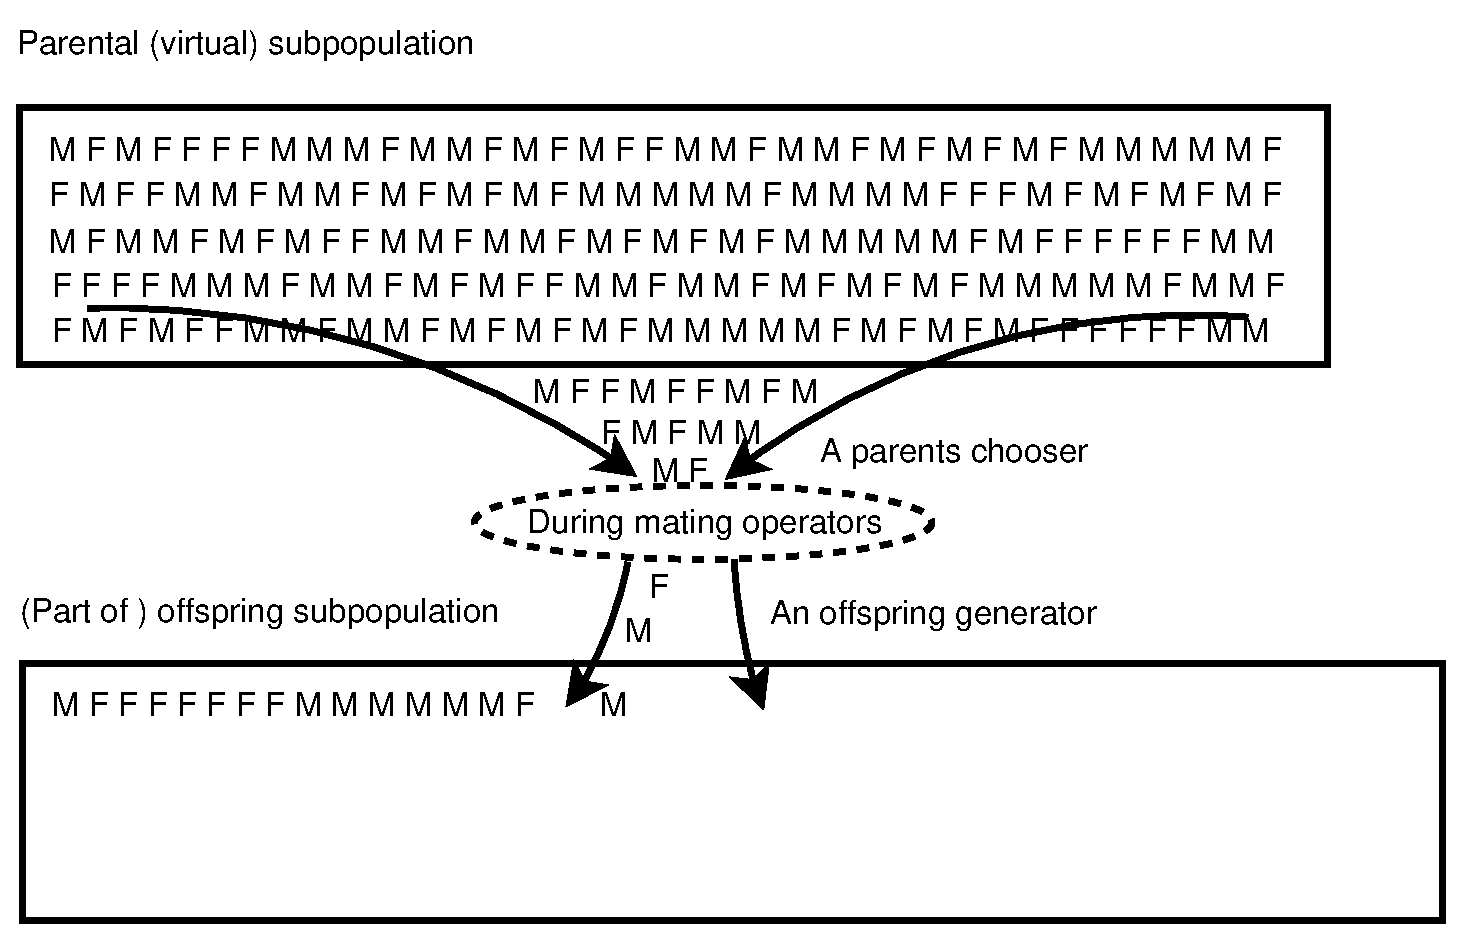
\includegraphics[width=0.9\textwidth]{figures/HomoMatingScheme}

A homogeneous mating scheme is responsible to choose parent(s) from
a subpopulation or a virtual subpopulation, and population part or
all of the corresponding offspring subpopulation. A parent chooser
is used to choose one or two parents from the parental generation,
and pass it to an offspring generator, which produces one or more
offspring. During mating operators such as taggers and Recombinator
can be applied when offspring is generated.
\end{figure}


\subsection{Control the size of the offspring generation\label{subsec:offspring-size}}

A mating scheme goes through each subpopulation and populates the
subpopulations of an offspring generation sequentially. The number
of offspring in each subpopulation is determined by the mating scheme,
following the following rules:
\begin{itemize}
\item A simuPOP mating scheme, by default, produces an offspring generation
that has the same subpopulation sizes as the parental generation.
This does not guarantee a constant population size because some operators,
such as a \texttt{Migrator} and \texttt{DiscardIf} can change population
or subpopulation sizes.
\item If fixed subpopulation sizes are given to parameter \texttt{subPopSize}.
A mating scheme will generate an offspring generation with specified
sizes even if an operator has changed parental population sizes.
\item A \textbf{demographic function} can be specified to parameter \texttt{subPopSize}.
This function should take one of the two forms \texttt{func(gen)}
or \texttt{func(gen, pop)} where \texttt{gen} is the current generation
number and \texttt{pop} is the parental population just before mating.
This function should return an array of new subpopulation sizes. A
single number can be returned if there is only one subpopulation.
The \texttt{simuPOP.demography} module provides a number of demography-related
functions for complex evolutionary secenarios. \textbf{Please consider
contributing to this module if you have implemented demographic models
for particular populations.}
\end{itemize}
The following examples demonstrate these cases. Example \ref{migrSize}
uses a default \texttt{RandomMating()} scheme that keeps parental
subpopulation sizes. Because migration between two subpopulations
are asymmetric, the size of the first subpopulation increases at each
generation, although the overall population size keeps constant. \lstinputlisting[caption={Free change of subpopulation sizes},label={migrSize}]{log/migrSize.log}

Example \ref{migrFixedSize} uses the same Migrator to move individuals
between two subpopulations. Because a constant subpopulation size
is specified, the offspring generation always has 500 and 1000 individuals
in its two subpopulations. Note that operators \texttt{Stat} and \texttt{PyEval}
are applied both before and after mating. It is clear that subpopulation
sizes changes before mating as a result of migration, although the
pre-mating population sizes vary because of uncertainties of migration.

\lstinputlisting[caption={Force constant subpopulation sizes},label={migrFixedSize}]{log/migrFixedSize.log}

Example \ref{demoFunc} uses a demographic function to control the
subpopulation size of the offspring generation. This example implements
a linear population expansion model but arbitrarily complex demographic
model can be implemented similarly.

\lstinputlisting[caption={Use a demographic function to control population size},label={demoFunc}]{log/demoFunc.log}

If the size of the offspring generation can not be determined directly
from generation number, you can pass the parental population as parameter
\texttt{pop} to the demographic function. For example, Example \ref{demoFunc1}
implements a demographic model where a population expand at random
numbers at each generation. \lstinputlisting[caption={Use parental population to determine the size of offspring population},label={demoFunc1}]{log/demoFunc1.log}

In all the above examples, migration and demographic changes are introduced
manually to influence the evolution of populations. However, the demographic
changes might be driven by other factors such as natural selection
so that it is difficult to predict the size of offspring generations
in advance. In this case, you can manually remove individuals from
parental (or offspring) populations using appropriate operators.

For example, a population in Example \ref{demoBySelection} suffers
from a sudden reduction of population size (due to perhaps a famine)
at generation 3, and a gradual reduction of population size (due to
perhaps an outburst of an infectious disease) after generation 5.
The first event is implemented using a \texttt{ResizeSubPops} operator
that directly shrink the population size in half. The second event
is implemented using a \texttt{MaPenetrance} and a \texttt{DiscardIf}
operator. The first operator assigns affection status of each individual
using a disease model that involves individual genotype. The second
operator discard all individuals that are affected with the disease.
Despite of these unfortunate events, the population tries to expand
exponentially with offspring population sizes set to 105\% of their
parental populations. \lstinputlisting[caption={Change of  population size caused by natural selection},label={demoBySelection}]{log/demoBySelection.log}

\subsection{Advanced use of demographic functions \label{subsec:Advanced-demo-func}{*}}

The parental population passed to a demographic function is usually
used to determine offspring population size from parental population
size. However, because this function is called immediately before
mating happens, it provides a good opportunity for you to prepare
the parental generation for mating. Such activities could generally
be done by operators, but operations related to demographic changes
could be done here. For example, Example \ref{advancedDemoFunc} uses
a demographic function to split populations at certain generation.
The advantage of this method over the use of a \texttt{SplitSubPops}
operator (for example as in Example \ref{splitByProp}) is that all
demographic information presents in the same function so you do not
have to worry about changing an operator when your demographic model
changes.  \lstinputlisting[caption={Use a demographic function to split parental population},label={advancedDemoFunc}]{log/advancedDemoFunc.log}

\subsection{Determine the number of offspring during mating\label{subsec:number-of-offspring}}

simuPOP by default produces only one offspring per mating event. Because
more parents are involved in the production of offspring, this setting
leads to larger effective population sizes than mating schemes that
produce more offspring at each mating event. However, various situations
require a larger family size or even varying family sizes. In these
cases, parameter \texttt{numOffspring} can be used to control the
number of offspring that are produced at each mating event. This parameter
takes the following types of inputs
\begin{itemize}
\item If a single number is given, \texttt{numOffspring} offspring are produced
at each mating event.
\item If a Python function is given, this function will be called each time
when a mating event happens. Generation number can be passed to this
function as parameter \texttt{gen} to allow different numbers of offspring
at different generations. A python generator function can also be
passed to provide an iterator interface to yield number of offspring
for all mating events.
\item If a tuple (or list) with more than one numbers is given, the first
number must be one of \texttt{GEOMETRIC\_DISTRIBUTION}, \texttt{POISSON\_DISTRIBUTION},
\texttt{BINOMIAL\_DISTRIBUTION} and \texttt{UNIFORM\_DISTRIBUTION},
with one or two additional parameters. 
\end{itemize}
The number of offspring in the last case will then follow a specific
statistical distribution. More specifically, 
\begin{itemize}
\item \texttt{numOffspring=(GEOMETRIC\_DISTRIBUTION, p)}: The number of
offspring for each mating event follows a geometric distribution with
mean $1/p$ and variance $\left(1-p\right)/p^{2}$: 
\[
\mbox{Pr}\left(k\right)=p\left(1-p\right)^{k-1}\;\textrm{ for }k\geq1
\]
\item \texttt{numOffspring=(POISSON\_DISTRIBUTION, p)}: The number of offspring
for each mating event follows a Poisson distribution with mean $p$
and variance $p$. The distribution is
\[
\mbox{Pr}\left(k\right)=\frac{p^{k}e^{-p}}{k!}\;\textrm{ for }k\geq0
\]
Note that, however, because families with zero offspring are ignored,
the distribution of the observed number of offspring (excluding zero)
follows a zero-truncated Poission distribution with probability
\[
\mbox{Pr}\left(k\right)=\frac{p^{k}e^{-p}}{k!\left(1-e^{-p}\right)}\;\textrm{ for }k\geq1
\]
The mean number of offspring is therefore $\frac{1}{1-e^{-p}}p$,
which is 2.31 for $p=2$.
\item \texttt{numOffspring=(BINOMIAL\_DISTRIBUTION, p, n): }The number of
offspring for each mating event follows a Binomial distribution with
mean $np$ and variance $np\left(1-p\right)$. 
\[
\mbox{Pr}\left(k\right)=\frac{n!}{k!\left(n-k\right)!}p^{k}\left(1-p\right)^{n-k}\;\textrm{ for }n\geq k\geq0
\]
Because families with zero offspring are ignored, the distribution
of the observed number of offspring (excluding zero) follows a zero-truncated
Bionimial distribution, with mean number of offspring being $\frac{np}{\left(1-p\right)^{n}}$.
\item \texttt{numOffspring=(UNIFORM\_DISTRIBUTION, a, b):} The number of
offspring for each mating event follows a discrete uniform distribution
with lower bound $a$ and upper bound $b$. 
\[
\mbox{Pr}\left(k\right)=\frac{1}{b-a+1}\;\textrm{ for }b\geq k\geq a
\]
The lower bound of this distribution can be \texttt{0} but is identical
to the case with $a=1$.
\end{itemize}
Example \ref{numOff} demonstrates how to use parameter \texttt{numOffspring}.
In this example, a function \texttt{checkNumOffspring} is defined.
It takes a mating scheme as its input parameter and use it to evolve
a population with 30 individuals. After evolving a population for
one generation, parental indexes are used to identify siblings, and
then the number of offspring per mating event.

\lstinputlisting[caption={Control the number of offspring per mating event.},label={numOff}]{log/numOff.log}

However, \textbf{the actual number of offspring can be less than specified
because offspring can be discarded during mating.} More specifically,
if any during-mating generator, such as a during-mating selector,
returns \texttt{False} during the production of offspring, the offspring
will be discarded so the total number of offspring will be reduced.
This is the case in the seventh case of Example \ref{numOff} where
offspring with certain genotypes have lower probabilities to survive.
If you would like to control size of families in the presence of natural
selection, you could set a larger \texttt{numOffspring} use a \texttt{OffspringTagger}
to mark the index of offspring, and discard offspring conditionally
using operator \texttt{DiscardIf} . Please refer to example \ref{OffspringTagger}
for details.

\subsection{Dynamic population size determined by number of offspring {*}}

What we have described so far requires you to determine the size of
offspring population in advance. Each mating event produces a number
of offspring that is determined by parameter \texttt{NumOffspring}.
The mating process stops when the offspring population is filled.
This works for most scenarios but there are cases where the offspring
population size is determined dynamically from a fixed number of mating
events with random number of offspring. For example, you might design
a mating scheme where all males in a population mate only once and
produce random number of offspring.

These kind of mating schemes can be simulated using a demographic
model that calculates offspring population size from pre-simulated
number of offspring for each family. More specifically, we
\begin{itemize}
\item Define a demogrphic function (model) that will be called before mating
happens.
\item This function determines and save the number of offspring for each
mating event, and return the total number of offspring as offspring
population size.
\item Pass a function or generator to parameter numOffspring to pass pre-determined
number of offspring. This function will be called each time when number
of offspring is needed.
\end{itemize}
The number of offspring could be saved and retrieved as global variable
but a more clever method is to store the numbers of offspring in a
demographic model (class). Example \ref{dynamicNumOff} demonstrates
this method by implementing a demographic model that simulate, save,
and return the number of offspring. Note that although we determine
the number of mating events from number of males in the parental population,
a random mating scheme will choose parents with replacement so it
is likely that some parents will be chosen multiple times while some
others are not chosen at all. Please refer to section ``Non-random
and customized mating schemes'' to learn how to define a mating scheme
that picks parents without replacement. \lstinputlisting[caption={Dynamic population size determined by number of offspring},label={dynamicNumOff}]{log/dynamicNumOff.log}

\subsection{Determine sex of offspring\label{subsec:offspring-sex}}

Because sex can influence how genotypes are transmitted (e.g. sex
chromosomes, haplodiploid population), simuPOP determines offspring
sex before it passes an offspring to a \emph{genotype transmitter}
(during-mating operator) to transmit genotype from parents to offspring.
The default \texttt{sexMode} in almost all mating schemes is \texttt{RandomSex},
in which case simuPOP assign \texttt{Male} or \texttt{Female} to offspring
with equal probability.

Other sex determination methods are also available:
\begin{itemize}
\item \texttt{sexMode=RANDOM\_SEX}: Sex is determined randomly, with equal
probability for \texttt{MALE} and \texttt{FEMALE}. This is the default
mode for sexual mating schemes such as random mating.
\item \texttt{sexMode=NO\_SEX}: Sex is not simulated so everyone is \texttt{MALE}.
This is the default mode for asexual mating schemes.
\item \texttt{sexMode=(PROB\_OF\_MALES, prob)}: Produce males with given
probability.
\item \texttt{sexMode=(NUM\_OF\_MALES, n)}: The first \texttt{n} offspring
in each family will be \texttt{Male}. If the number of offspring at
a mating event is less than or equal to \texttt{n}, all offspring
will be male. 
\item \texttt{sexMode=(NUM\_OF\_FEMALES, n)}: The first \texttt{n} offspring
in each family will be \texttt{Female}.
\item \texttt{sexMode=(SEQUENCE\_OF\_SEX, s1, s2, ...)}: Use sequence \texttt{s1},
\texttt{s2}, ... for offspring in each mating event.
\item \texttt{sexMode=(GLOBAL\_SEQUENCE\_OF\_SEX, s1, s2, ...)}: Use sequence
\texttt{s1}, \texttt{s2}, ... for all offspring in a subpopulation.
Because other mode of sex determination works within each mating event,
this is the only way to ensure proportion of sex in a subpopulation.
For example, \texttt{(GLOBAL\_SEQUENCE\_OF\_SEX, MALE, FEMALE)} will
gives \texttt{MALE} and \texttt{FEMALE} iteratively to all offspring,
making sure there are equal number of males and females (if there
are even number of offspring).
\item \texttt{sexMode=func} or \texttt{sexMode=generator\_func}: In this
last case, a Python function or a Python generator function can be
specified to provide sex to each offspring. The function is called
whenever an offspring is created. The generator function is called
for each subpopulation, and provides an iterator that provides sex
for all offspring in a subpopulation.
\end{itemize}
\texttt{NumOfMales} and \texttt{NumOfFemales} are useful in theoretical
studies where the sex ratio of a population needs to be controlled
strictly, or in special mating schemes, usually for animal populations,
where only a certain number of male or female Individuals are allowed
in a family. It worth noting that a genotype transmitter can override
specified offspring sex. This is the case for \texttt{CloneGenoTransmitter}
where an offspring inherits both genotype and sex from his/her parent. 

Example \ref{sexMode} demonstrates how to use parameter \texttt{sexMode}.
In this example, a function \texttt{checkSexMode} is defined. It takes
a mating scheme as its input parameter and use it to evolve a population
with 40 individuals. After evolving a population for one generation,
sexes of all offspring are returned as a string.

\lstinputlisting[caption={Determine the sex of offspring},label={sexMode}]{log/sexMode.log}

\subsection{Monogamous mating}

Monogamous mating (monogamy) in simuPOP refers to mating schemes in
which each parent mates only once. In an asexual setting, this implies
parents are chosen without replacement. In sexual mating schemes,
this means that parents are chosen without replacement, they have
only one spouse during their life time so that all siblings have the
same parents (no half-sibling).

simuPOP provides a diploid sexual monogamous mating scheme \texttt{MonogamousMating}.
However, without careful planning, this mating scheme can easily stop
working due to the lack of parents. For example, if a population has
40 males and 55 females, only 40 successful mating events can happen
and result in 40 offspring in the offspring generation. \texttt{MonogamousMating}
will exit if the offspring generation is larger than 40.

Example \ref{monogamous} demonstrates one scenario of using a monogamous
mating scheme where sex of parents and offspring are strictly specified
so that parents will not be exhausted. The sex initializer \texttt{InitSex}
assigns exactly 10 males and 10 females to the initial population.
Because of the use of \texttt{numOffspring=2, sexMode=(NUM\_OF\_MALES,
1)}, each mating event will produce exactly one male and one female.
Unlike a random mating scheme that only about 80\% of parents are
involved in the production of an offspring population with the same
size, this mating scheme makes use of all parents. \lstinputlisting[caption={Sexual monogamous mating},label={monogamous}]{log/monogamous.log}

\subsection{Polygamous mating}

In comparison to monogamous mating, parents in a polygamous mate with
more than one spouse during their life-cycle. Both \emph{polygany}
(one man has more than one wife) and \texttt{\emph{polyandry}} (one
woman has more than one husband) are supported.

Other than regular parameters such as \texttt{numOffspring}, mating
scheme \texttt{PolygamousMating} accepts parameters \texttt{polySex}
(default to \texttt{Male}) and \texttt{polyNum} (default to 1). During
mating, an individual with \texttt{polySex} is selected and then mate
with \texttt{polyNum} randomly selected spouse. Example \ref{polygamous}
demonstrates the use of this mating schemes. Note that this mating
scheme support natural selection, but does not yet handle varying
\texttt{polyNum} and selection of parents without replacement. \lstinputlisting[caption={Sexual polygamous mating},label={polygamous}]{log/polygamous.log}

\subsection{Asexual random mating}

Mating scheme \texttt{RandomSelection} implements an asexual random
mating scheme. It randomly select parents from a parental population
(with replacement) and copy them to an offspring generation. Both
genotypes and sex of the parents are copied because genotype and sex
are sometimes related. This mating scheme can be used to simulate
the evolution of haploid sequences in a standard haploid Wright-Fisher
model.

Example \ref{RandomSelection} applies a \texttt{RandomSelection}
mating scheme to a haploid population with 100 sequences. A \texttt{parentTagger}
is used to track the parent of each individual. Although sex information
is not used in this mating scheme, Individual sexes are initialized
and passed to offspring.

\lstinputlisting[caption={Asexual random mating},label={RandomSelection}]{log/RandomSelection.log}

\subsection{Mating in haplodiploid populations}

Male individuals in a haplodiploid population are derived from unfertilized
eggs and thus have only one set of chromosomes. Mating in such a population
is handled by a special mating scheme called \texttt{haplodiplodMating}.
This mating scheme chooses a pair of parents randomly and produces
some offspring. It transmit maternal chromosomes and paternal chromosomes
(the only copy) to female offspring, and only maternal chromosomes
to male offspring. Example \ref{HaplodiploidMating} demonstrates
how to use this mating scheme. It uses three initializers because
sex has to be initialized before two other intializers can initialize
genotype by sex. \lstinputlisting[caption={Random mating in haplodiploid populations},label={HaplodiploidMating}]{log/HaplodiploidMating.log}

Note that this mating scheme does not support recombination and the
standard Recombinator does not work with haplodiploid populations.
Please refer to the next Chapter for how to define a customized genotype
transmitter to handle such a situation.

\subsection{Self-fertilization}

Some plant populations evolve through self-fertilization. That is
to say, a parent fertilizes with itself during the production of offspring
(seeds). In a \texttt{SelfMating} mating scheme, parents are chosen
randomly (one at a time), and are used twice to produce two homologous
sets of offspring chromosomes. The standard Recombinator can be used
with this mating scheme. Example \ref{SelfMating} initializes each
chromosome with different alleles to demonstrate how these alleles
are transmitted in this population.

\lstinputlisting[caption={Selfing mating scheme},label={SelfMating}]{log/SelfMating.log}

\subsection{Heterogeneous mating schemes {*}}

Different groups of individuals in a population may have different
mating patterns. For example, individuals with different properties
can have varying fecundity, represented by different numbers of offspring
generated per mating event. This can be extended to aged populations
in which only adults (may be defined by age > 20 and age < 40) can
produce offspring, where other individuals will either be copied to
the offspring generation or die.

A heterogeneous mating scheme (\texttt{HeteroMating}) accepts a list
of mating schemes that are applied to different subpopulation or virtual
subpopulations. If multiple mating schemes are applied to the same
subpopulation, each of them only populate part of the offspring subpopulation.
This is illustrated in Figure \ref{fig:heterogenous-mating}.

\begin{figure}[h]
\caption{\label{fig:heterogenous-mating}Illustration of a heterogeneous mating
scheme}

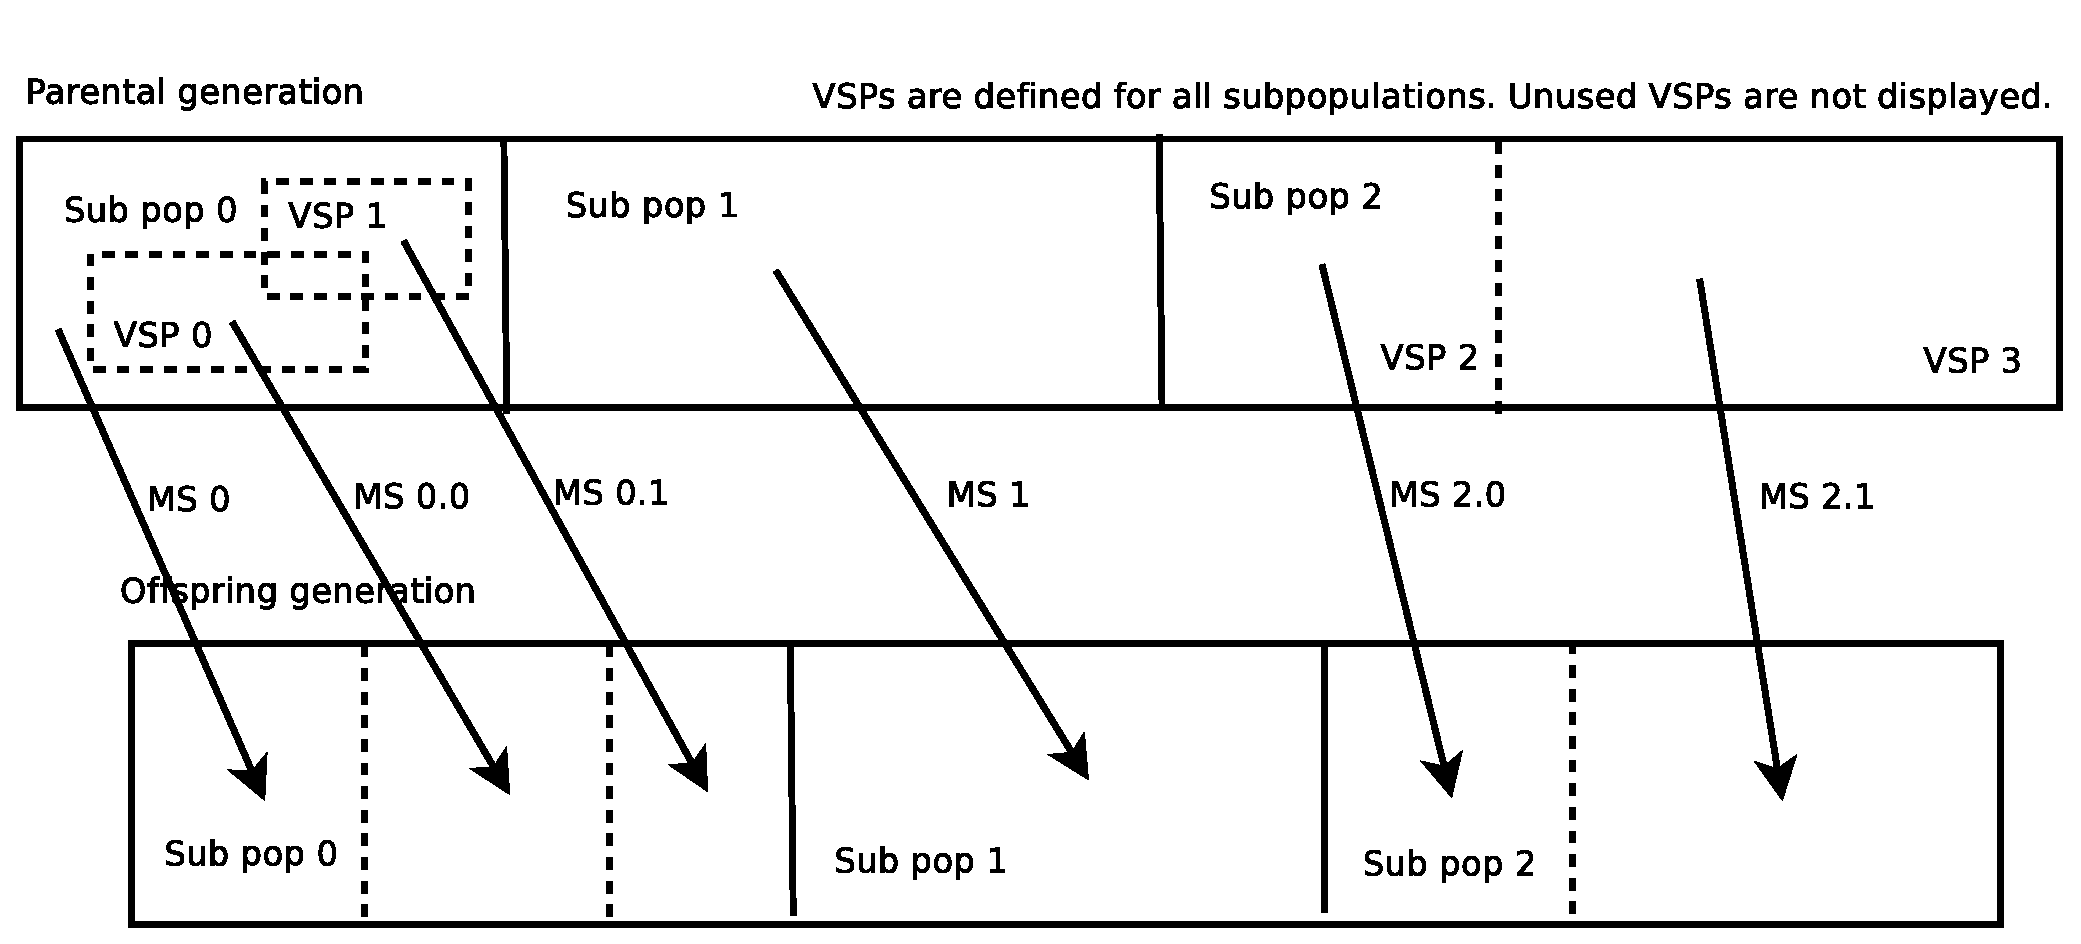
\includegraphics[width=1\textwidth]{figures/MatingScheme}

A heterogeneous mating scheme that applies homogeneous mating schemes
MS0, MS0.0, MS0.1, MS1, MS2.0 and MS2.1 to subpopulation 0, the first
and second virtual subpopulation in subpopulation 0, subpopulation
1, the first and second virtual subpopulation in subpopulation 2,
respectively. Note that VSP 0 and 1 in subpopulation 0 overlap, and
do not add up to subpopulation 0.
\end{figure}

For example, Example \ref{hateroMatingSP} applies two random mating
schemes to two subpopulations. The first mating scheme produces two
offspring per mating event, and the second mating scheme produces
four.

\lstinputlisting[caption={Applying different mating schemes to different subpopulations },label={hateroMatingSP}]{log/HeteroMatingSP.log}

The real power of heterogeneous mating schemes lies on their ability
to apply different mating schemes to different virtual subpopulations.
For example, due to different micro-environmental factors, plants
in the same population may exercise both self and cross-fertilization.
Because of the randomness of such environmental factors, it is difficult
to divide a population into self and cross-mating subpopulations.
Applying different mating schemes to groups of individuals in the
same subpopulation is more appropriate.

Example \ref{hateroMatingVSP} applies two mating schemes to two VSPs
defined by proportions of individuals. In this mating scheme, 20\%
of individuals go through self-mating and 80\% of individuals go through
random mating. This can be seen from the parental indexes of individuals
in the offspring generation: individuals whose \texttt{mother\_idx}
are \texttt{-1} are genetically only derived from their fathers. 

It might be surprising that offspring resulted from two mating schemes
mix with each other so the same VSPs in the next generation include
both selfed and cross-fertilized offspring. If this not desired, you
can set parameter \texttt{shuffleOffspring=False} in \texttt{HeteroMating}().
Because the number of offspring that are produced by each mating scheme
is proportional to the size of parental (virtual) subpopulation, the
first 20\% of individuals that are produced by self-fertilization
will continue to self-fertilize.

\lstinputlisting[caption={Applying different mating schemes to different virtual subpopulations },label={hateroMatingVSP}]{log/HeteroMatingVSP.log}

Because there is no restriction on the choice of VSPs, mating schemes
can be applied to overlapped (virtual) subpopulations. For example,

\begin{lstlisting}
HeteroMating(
    matingSchemes = [
        SelfMating(subPops=[(0, 0)]),
        RandomMating(subPops=0)
        ]
)
\end{lstlisting}
will apply SelfMating to the first 20\% individuals, and RandomMating
will be applied to all individuals. Similarly,
\begin{lstlisting}
HeteroMating(
    matingSchemes = [
        SelfMating(subPops=0),
        RandomMating(subPops=0)
        ]
)
\end{lstlisting}
will allow all individuals to be involved in both \texttt{SelfMating}
and \texttt{RandomMating}.

This raises the question of how many offspring each mating scheme
will produce. By default, the number of offspring produced will be
proportional to the size of parental (virtual) subpopulations. In
the last example, because both mating schemes are applied to the same
subpopulation, half of all offspring will be produced by selfing and
the other half will be produced by random mating.

This behavior can be changed by a weighting scheme controlled by parameter
\texttt{weight} of each homogeneous mating scheme. Briefly speaking,
a positive weight will be compared against other mating schemes. a
negative weight is considered proportional to the existing (virtual)
subpopulation size. Negative weights are considered before positive
or zero weights.

This weighting scheme is best explained by an example. Assuming that
there are three mating schemes working on the same parental subpopulation
\begin{itemize}
\item Mating scheme A works on the whole subpopulation of size 1000
\item Mating scheme B works on a virtual subpopulation of size 500
\item Mating scheme C works on another virtual subpopulation of size 800
\end{itemize}
Assuming the corresponding offspring subpopulation has $N$ individuals, 
\begin{itemize}
\item If all weights are 0, the offspring subpopulation is divided in proportion
to parental (virtual) subpopulation sizes. In this example, the mating
schemes will produce $\frac{10}{23}N$, $\frac{5}{23}N$, $\frac{8}{23}N$
individuals respectively.
\item If all weights are negative, they are multiplied to their parental
(virtual) subpopulation sizes. For example, weight (-1, -2, -0.5)
will lead to sizes (1000, 1000, 400) in the offspring subpopulation.
If $N\ne2400$ in this case, an error will be raised.
\item If all weights are positive, the number of offspring produced from
each mating scheme is proportional to these weights. For example,
weights (1, 2, 3) will lead to $\frac{1}{6}N$, $\frac{2}{6}N$, $\frac{1}{3}N$
individuals respectively. In this case, 0 weights will produce no
offspring.
\item If there are mixed positive and negative weights, the negative weights
are processed first, and the rest of the individuals are divided using
non-negative weights. For example, three mating schemes with weights
(-0.5, 2, 3) will produce 500, $\frac{2}{5}\left(N-500\right)$, $\frac{3}{5}\left(N-500\right)$
individuals respectively.
\end{itemize}
The last case is demonstrated in Example \ref{HeteroMatingWeight}
where three random mating schemes are applied to subpopulation \texttt{0},
virtual subpopulation\texttt{ (0, 0)} and virtual subpopulation \texttt{(0,
1)}, with weights \texttt{-}0.5, \texttt{2}, and \texttt{3} respectively.
This example uses an advanced features that will be described in the
next section. Namely, three during-mating Python operators are passed
to each mating scheme to mark their offspring with different numbers.

\lstinputlisting[caption={A weighting scheme used by heterogeneous mating schemes.},label={HeteroMatingWeight}]{log/HeteroMatingWeight.log}

As a special case that can be quite annoying during the simulation
of small populations, a (virtual) subpopulation can have no male and/or
female. If the parental (virtual) subpopulation is empty, it will
produce no offspring regardless of its weight. However, if the parental
(virtual) subpopulation is not empty, it will be expected to produce
some offspring, which is not possible if a sexual mating scheme is
used. In this case, you can use a parameter \texttt{weightBy} to specify
how parental (virtual) population sizes are calculated. This parameter
accepts values \texttt{ANY\_SEX} (default), \texttt{MALE\_ONLY}, \texttt{FEMALE\_ONLY},
\texttt{PAIR\_ONLY}, and use all individuals, number of male individuals,
number of female individuals, and number of male/female pairs (basically
the less of numbers of males and females) as the size of parental
(virtual) subpopulation, respectively. When \texttt{weightBy=PAIR\_ONLY}
is used, parental (virtual) subpopulations with only males or females
will appear to be empty and produce no offspring. Note that in this
mode (also \texttt{MALE\_ONLY}, \texttt{FEMALE\_ONLY}), the perceived
parental population sizes are no longer the actual parental population
sizes so you might need to adjust parameter \texttt{weight} (e.g.
\texttt{weight=-2}) to produce correct number of offspring.

\subsection{Conditional mating schemes}

A \texttt{ConditionalMating} mating scheme allows you to apply different
mating schemes to populations with different properties. The condition
can be a constant (True or False), an expression that will be evaluated
in the local namspace of the parental population, or a function that
can take parental population as its input paramter (with parameter
name \texttt{pop}). 

Using variable \texttt{rep} and \texttt{gen} in the local namespace
of the parental population, we can use this mating scheme to apply
different mating schemes to different replicates and/or at different
generations. For example, \ref{matingSchemeByRepAndGen} simulates
the evolution of three replicates. The first replicate uses regular
mating scheme, the third replicate uses a mating scheme that produces
70\% of males, and the second replicate do this only for the first
5 generations. Because there are three cases, a nested \texttt{ConditionalMating}
is used.

\lstinputlisting[caption={Apply different mating schemes for different replicates at different generations},label={matingSchemeByRepAndGen}]{log/matingSchemeByRepAndGen.log}

A function can be passed as the condition of a \texttt{ConditionalMating}
mating scheme. This allows you to apply operators such as \texttt{Stat}
to examine the condition of populations more closely and determine
which mating scheme to use.

\section{Simulator}

A simuPOP simulator evolves one or more copies of a population forward
in time, subject to various operators. Although a population could
evolve by itself using function \texttt{Population.evolve}, a simulator
with one replicate is actually used.

\subsection{Add, access and remove populations from a simulator}

A simulator could be created by one or more replicates of a list of
populations. For example, you could create a simulator from five replicates
of a population using 
\begin{lstlisting}
Simulator(pop, rep=5)
\end{lstlisting}
or from a list of populations using 
\begin{lstlisting}
Simulator([pop, pop1, pop2])
\end{lstlisting}
. \texttt{pop}, \texttt{pop1} and \texttt{pop2} do not have to have
the same genotypic structure. In order to avoid duplication of potentially
large populations, a population is by default \emph{stolen} after
it is used to create a simulator. If you would like to keep the populations,
you could set parameter \texttt{stealPops} to \texttt{False} so that
the populations will be copied to the simulator. Populations in a
simulator can be added or removed using functions \texttt{Simulator.add()}
and \texttt{Simulator.extract(idx)}.

When a simulator is created, you can access populations in this simulator
using function \texttt{Simulator.population(idx)} or iterate through
all populations using function \texttt{Simulator.populations()}. These
functions return references to the populations so that you can access
populations. Modifying these references will change the corresponding
populations within the simulator. The references will become invalid
once the simulator object is destoryed. 

Example \ref{Simulator} demonstrates different ways to create a simulator
and how to access populations within it.

\lstinputlisting[caption={Create a simulator and access populations},label={Simulator}]{log/Simulator.log}

\subsection{Number of generations to evolve}

A simulator usually evolves a specific number of generations according
to parameter \texttt{gen} of the \texttt{evolve} function. A generation
number is used to track the number of generations a simulator has
evolved. Because a new population has generation number 0, a population
would be at the beginning of generation $n$ after it evolves $n$
generations. The generation number would increase if the simulator
continues to evolve. During evoluting, variables \texttt{rep} (replicate
number) and \texttt{gen} (current generation number) are set to each
population's local namespace.

It is not always possible to know in advance the number of generations
to evolve. For example, you may want to evolve a population until
a specific allele gets fixed or lost in the population. In this case,
you can let the simulator run indefinitely (do not set the \texttt{gen}
parameter) and depend on a \emph{terminator }to terminate the evolution
of a population. The easiest method to do this is to use population
variables to track the status of a population, and use a \texttt{TerminateIf}
operator to terminate the evolution according to the value of an expression.
Example \ref{simuGen} demonstrates the use of such a terminator,
which terminates the evolution of a population if allele 0 at locus
5 is fixed or lost. It also shows the application of an interesting
operator \texttt{IfElse}, which applies an operator, in this case
\texttt{PyEval}, only when an expression returns \texttt{True}. Note
that this example calls the \texttt{simulator.evolve} function twice.
The first call does not specify a mating scheme so a default empty
mating scheme (\texttt{MatingScheme}) that does not transmit genotype
is used. Populations start from the beginning of the fifth generation
when the second \texttt{simulator.evole} function is called.

The generation number is stored in each Population using population
variable \texttt{gen}.You can access these numbers from a simulator
using function \texttt{Simulator.dvars(idx)} or from a population
using function \texttt{Population.dvars()}. If needed, \textbf{you
can reset generation numbers by changing these variables.}

\lstinputlisting[keywordstyle={\ttfamily},caption={Generation number of a simulator},label={simuGen}]{log/simuGen.log}

\subsection{Evolve populations in a simulator}

There are a number of rules about when and how operators are applied
during the evolution of a population. In summary, in the order at
which operators are processed and applied,
\begin{itemize}
\item Operators specified in parameter \texttt{initOps} of function \texttt{Simulator.evolve}
will be applied to the initial population before evolution, subject
to replicate applicability restraint specified by parameter \texttt{reps}.
\item Operators specified in parameter \texttt{preOps} of function \texttt{Simulator.evolve}
will be applied to the parental population at each generation, subject
to replicate and generation applicability restraint specified by parameters
\texttt{begin}, \texttt{end}, \texttt{step}, \texttt{at}, and \texttt{reps}.
\item During-mating operators specified in the \texttt{ops} parameter of
a mating scheme will be called during mating to transmit genotype
(and possibly information fields etc) from parental to offspring,
subject to replicate and generation applicability restraint specified
by parameters \texttt{begin}, \texttt{end}, \texttt{step}, \texttt{at},
and \texttt{reps}. 
\item Operators specified in parameter postOps of function \texttt{Simulator.evolve}
will be applied to the offspring population at each generation, subject
to replicate and generation applicability restraint specified by parameters
\texttt{begin}, \texttt{end}, \texttt{step}, \texttt{at}, and \texttt{reps}.
\item Operators specified in parameter \texttt{finalOps} of function \texttt{Simulator.evolve}
will be applied to the final population after evolution, subject to
replicate applicability restraint specified by parameter \texttt{reps}.
\end{itemize}
Figure \ref{fig:operator-orders} illustrated how operators are applied
to an evolutionary process. It worth noting that a default during-mating
operator is defined for each mating scheme. User-specfied operators
will \textbf{replace} the default operator so you need to explicitly
specify the default operator if you intent to add another one.

\begin{figure}[h]
\caption{\label{fig:operator-orders}Orders at which operators are applied
during an evolutionary process}

\includegraphics[width=0.8\textwidth]{figures/operators}
\end{figure}

If you suspect that your simulation is not running as expected, you
can have a close look at your evolutionary process by setting the
\texttt{dryrun} parameter of an \texttt{evolve} function to \texttt{True},
or by calling function \texttt{describeEvolProcess()}. This function
takes the same set of parameters as \texttt{Simulator.evolve()} and
returns a description of the evolution process, which might help you
identify misuse of operators.

\lstinputlisting[caption={describe an evolutionary process},label={describe}]{log/describe.log}

\section{Non-random and customized mating schemes {*}}

\subsection{The structure of a homogeneous mating scheme {*}}

A \emph{homogeneous mating scheme} (\texttt{HomoMating}) populates
an offspring generation as follows:
\begin{enumerate}
\item Create an empty offspring population (generation) with appropriate
size. Parental and offspring generation can differ in size but they
must have the same number of subpopulations.
\item For each subpopulation, repeatedly choose a parent or a pair of parents
from the parental generation. This is done by a simuPOP object called
a \textbf{parent chooser}.
\item One or more offspring are produced from the chosen parent(s) and are
placed in the offspring population. This is done by a simuPOP \textbf{offspring
generator}. An offspring generator uses one or more during-mating
operators to transmit parental genotype to offspring. These operators
are called \textbf{genotype transmitters}.
\item After the offspring generation is populated, it will replace the parental
generation and becomes the present generation of a population.
\end{enumerate}
To define a homogeneous mating scheme, you will need to provide a
\texttt{chooser} (a \emph{parent chooser} that is responsible for
choosing one or two parents from the parental generation) and a \texttt{generator}
(an \emph{offspring generator} that is responsible for generating
a number of offspring from the chosen parents). For example, a \texttt{selfingMating}
mating scheme uses a \texttt{RandomParentChooser} to choose a parent
randomly from a population, possibly according to individual fitness,
it uses a standard \texttt{OffspringGenerator} that uses a \texttt{selfingOffspringGenerator}
to transmit genotype. The constructor of \texttt{HomoMating} also
accepts parameters \texttt{subPopSize} (parameter to control offspring
subpopulation sizes), \texttt{subPops} (applicable subpopulatiosn
or virtual subpopulations), and \texttt{weight} (weighting parameter
when used in a heterogeneous mating scheme). When this mating scheme
is applied to the whole population, \texttt{subPopSize} is used to
determine the subpopulation sizes of the offspring generation (see
Section \ref{subsec:offspring-size} for details), parameters \texttt{subPops}
and \texttt{weight} are ignored. Otherwise, the number of offspring
this mating scheme will produce is determined by the heterogeneous
mating scheme.

Example \ref{RandomMating} demonstrates how the most commonly used
mating scheme, the diploid sexual \texttt{RandomMating} mating scheme
is defined in \texttt{simuPOP.py}. This mating scheme uses a \texttt{RandomParentsChooser}
with replacement, and a standard \texttt{OffspringGenerator} using
a default \texttt{MendelianGenoTransmitter}. \lstinputlisting[firstline=2,caption={Define a random mating scheme},label={RandomMating}]{log/RandomMating.py}

Different parent choosers and offspring generators can be combined
to define a large number of homogeneous mating schemes. Some of the
parent choosers return one parent so they work with offspring generators
that need one parent (e.g. selfing or clone offspring generator);
some of the parent choosers return two parents so they work with offspring
generators that need two parents (e.g. Mendelian offspring generator).
For example, the standard \texttt{SelfMating} mating scheme uses a
\texttt{RandomParentChooser} but you can easily use a \texttt{SequentialParentChooser}
to choose parents sequentially and self-fertilize parents one by one.
This is demonstrated in Example \ref{sequentialSelfing}. \lstinputlisting[caption={Define a sequential selfing mating scheme},label={sequentialSelfing}]{log/sequentialSelfing.log}

\subsection{Offspring generators {*}}

An \texttt{OffspringGenerator} accepts a parameters \texttt{ops} (a
list of during-mating operators), \texttt{numOffspring} (control number
of offspring per mating event) and \texttt{sexMode} (control offspring
sex). We have examined the last two parameters in detail in sections
\ref{subsec:number-of-offspring} and \ref{subsec:offspring-sex}. 

The most tricky parameter is the \texttt{ops} parameter. It accepts
a list of during mating operators that are used to transmit genotypes
from parent(s) to offspring and/or set individual information fields.
The standard \texttt{OffspringGenerator} does not have any default
operator so no genotype will be transmitted by default. All stock
mating schemes use a default genotype transmitter. (e,g, a \texttt{MendelianGenoTransmitter}
in Example \ref{RandomMating} is passed to the offspring generator
used in \texttt{RandomMating}). Note that you need to specify all
needed operators if you use parameter \texttt{ops} to change the operators
used in a mating scheme (see Example \ref{HeteroMatingWeight}). That
is to say, you can use \texttt{ops=Recombinator()} to replace a default
\texttt{MendelianGenoTransmitter()}, but you have to use \texttt{ops={[}IdTagger(),
MendelianGenoTransmitter(){]}} if you would like to add a during-mating
operator to the default one.

Another offspring generator is provided in simuPOP. This \texttt{ControlledOffspringGenerator
}is used to control an evolutionary process so that the allele frequencies
at certain loci follows some pre-simulated \emph{frequency trajectories}.
Please refer to \citet{Peng2007a} for rationals behind such an offspring
generator and its applications in the simulation of complex human
diseases.

Example \ref{controlledOffGenerator} demonstrates the use of such
a controlled offspring generator. Instead of using a realistic frequency
trajectory function, it forces allele frequency at locus 5 to increase
linearly. In contrast, the allele frequency at locus 15 on the second
chromosome oscillates as a result of genetic drift. Note that the
random mating version of this mating scheme is defined in simuPOP
as \texttt{ControlledRandomMating}.

\lstinputlisting[caption={A controlled random mating scheme},label={controlledOffGenerator}]{log/controlledOffGenerator.log}

\subsection{Genotype transmitters {*}\label{subsec:Pre-defined-genotype-transmitters}}

Although any during mating operators can be used in parameter \texttt{ops
}of an offspring generator, those that transmit genotype from parents
to offspring are customarily called \textbf{genotype transmitters}.
simuPOP provides a number of genotype transmitters including clone,
Mendelian, selfing, haplodiploid, genotype transmitter, and a Recombinator.
They are usually used implicitly in a mating scheme, but they can
also be used explicitly.

Although simuPOP provides a number of genotype transmitters, they
may still be cases where customized genotype transmitter is needed.
For example, a Recombinator can be used to recombine parental chromosomes
but it is well known that male and female individuals differ in recombination
rates. How can you apply two different Recombinators to male and female
Individuals separately?

An immediate thought can be the use of virtual subpopulations. If
you apply two random mating schemes to two virtual subpopulations
defined by sex, \texttt{RandomParentsChooser} will not work because
no opposite sex can be found in each virtual subpopulation. In this
case, a customized genotype transmitter can be used.

A customized genotype transmitter is only a Python during-mating operator.
Although it is possible to define a function and use a PyOperator
directly (Example \ref{PyOperator}), it is much better to derive
an operator from PyOperator, as the case in Example \ref{newOperator}. 

Example \ref{sexSpecificRec} defines a \texttt{sexSpecificRecombinator}
that uses, internally, two different Recombinators to recombine male
and female parents. The key statement is the \texttt{PyOperator.\_\_init\_\_}
line which initializes a Python operator with given function \texttt{self.transmitGenotype}.
Example \ref{sexSpecificRec} outputs the population in two generations.
You should notice that paternal chromosome are not recombined when
they are transmitted to offspring.

\lstinputlisting[caption={A customized genotype transmitter for sex-specific recombination},label={sexSpecificRec}]{log/sexSpecificRec.log}

\subsection{A Python parent chooser {*}}

Parent choosers are responsible for choosing one or two parents from
a parental (virtual) subpopulation. simuPOP defines a few parent choosers
that choose parent(s) sequentially, randomly (with or without replacement),
or with additional conditions. Some of these parent choosers support
natual selection. We have seen sequential and random parent choosers
in Examples \ref{sequentialSelfing} and \ref{controlledOffGenerator}.
Please refer to the simuPOP reference manual for details about these
objects.

A parent choosing scheme can be quite complicated in reality. For
example, salamanders along a river may mate with their neighbors and
form several subspecies. This behavior cannot be readily simulated
using any pre-define parent choosers so a hybrid parent chooser \texttt{PyParentsChooser()}
should be used.

A \texttt{PyParentsChooser} accepts a user-defined Python generator
function, instead of a normal python function, that returns a parent,
or a pair of parents repeatedly. Briefly speaking, when a generator
function is called, it returns a \emph{generator} object that provides
an iterator interface. Each time when this iterator iterates, this
function resumes where it was stopped last time, executes and returns
what the next \emph{yield} statement returns. For example, example
\ref{generator} defines a function that calculate $f\left(k\right)=\sum_{i=1}^{k}\frac{1}{i}$
for $k=1,...,5$. It does not calculate each $f\left(k\right)$ repeatedly
but returns $f\left(1\right)$, $f\left(2\right)$, ... sequentially.

\lstinputlisting[caption={A sample generator function},label={generator}]{log/generator.log}

A \texttt{PyParentsChooser} accepts a parent generator function, which
takes a population and a subpopulation index as parameters. When this
parent chooser is applied to a subpopulation, it will call this generator
function and ask the generated generator object repeated for either
a parent, or a pair of parents (\emph{references to individual objects
or indexes relative to a subpopulation}). Note that \texttt{PyParentsChooser}
does not support virtual subpopulation but you can mimic the effect
by returning only parents from certain virtual subpopulations.

Example \ref{PyParentsChooser} implements a hybrid parent chooser
that chooses parents with equal social status (\texttt{rank}). In
this parent chooser, all males and females are categorized by their
sex and social status. A parent is chosen randomly, and then his/her
spouse is chosen from females/males with the same social status. The
rank of their offspring can increase or decrease randomly. It becomes
obvious now that whereas a python function can return random male/female
pair, the generator interface is much more efficient because the identification
of sex/status groups is done only once.

\lstinputlisting[caption={A hybrid parent chooser that chooses parents by their social status},label={PyParentsChooser}]{log/PyParentsChooser.log}

Built-in parent choosers could be used in a \texttt{PyParentsChooser}
to choose parents. The parent chooser needs to be initialized with
the parental population and subpopulation index. Calling the \texttt{chooseParents}
function repeatedly will return pairs of individuals from the population
(\texttt{None} will be returned for one of the parents if the parent
chooser only returns one parent). The use of built-in parent choosers
can improve the performance of your \texttt{PyParentsChooser}, especially
for complex selection patterns (e.g. with natural selection). For
example, \ref{BuiltInParentsChooser} implements a similar mating
scheme as Example \ref{PyParentsChooser} but uses a \texttt{RandomParentChooser}
to choose males randomly. 

\lstinputlisting[caption={Use built-in parent choosers in a Python parent chooser},label={BuiltInParentsChooser}]{log/BuiltInParentsChooser.log}

\subsection{Using C++ to implement a parent chooser {*}{*}\label{subsec:Using-C++}}

A user defined parent chooser can be fairly complex and computationally
intensive. For example, if a parent tends to find a spouse in his/her
vincinity, geometric distances between all qualified individuals and
a chosen parent need to be calculated for each mating event. If the
optimization of the parent chooser can speed up the simulation significantly,
it may be worthwhile to write the parent chooser in C++. 

Although it is feasible, and sometimes easier to derive a class from
class \texttt{ParentChooser} in mating.h (.cpp), modifying simuPOP
source code is not recommended because you would have to modify a
new version of simuPOP whenever you upgrade your simuPOP distribution.
Implementing your parent choosing algorithm in another Python module
is preferred.

The first step is to write your own parent chooser in C/C++. Basically,
you will need to pass all necessary information to the C++ level and
implement an algorithm to choose parents randomly. Although simple
function based solutions are possible, a C++ level class such as the
\texttt{myParentsChooser }class defined in Example \ref{parentChooseHeader}
is recommended. This class is initialized with indexes of male and
female individuals and use a function \texttt{chooseParents} to return
a pair of parents randomly. This parent chooser is very simple but
more complicated parent selection scenarios can be implemented similarly.

\lstinputlisting[language=C,caption={Implement a parent chooser in C++},label={parentChooseHeader}]{log/myParentsChooser.h}

The second step is to wrap your C++ functions and classes to a Python
module. There are many tools available but SWIG (\texttt{www.swig.org})
is arguably the most convenient and powerful one. To use SWIG, you
will need to prepare an interface file, which basically tells SWIG
which functions and classes you would like to expose and how to pass
parameters between Python and C++. Example \ref{parentsChooserInterface}
lists an interface file for the C++ class defined in Example \ref{parentChooseHeader}.
Please refer to the SWIG reference manual for details.

\lstinputlisting[language=Awk,caption={An interface file for the myParentsChooser class},label={parentsChooserInterface}]{log/myParentsChooser.i}

The exact procedure to generate and compile a wrapper file varies
from system to system, and from compiler to compiler. Fortunately,
the standard Python module setup process supports SWIG. All you need
to do is to write a Python \texttt{setup.py} file and let the \texttt{distutil}
module of Python handle all the details for you. A typical \texttt{setup.py}
file is demonstrated in Example \ref{parentsChooserSetup}.

\lstinputlisting[caption={Building and installing the myParentsChooser module},label={parentsChooserSetup}]{log/setup.py}

You parent chooser can now be compiled and installed using the standard
Python \texttt{setup.py} commands such as

\begin{lstlisting}
python setup.py install
\end{lstlisting}

Please refer to the Python reference manual for other building and
installation options. Note that Python 2.4 and earlier do not support
option swig\_opts well so you might have to pass these options using
command

\begin{lstlisting}
python setup.py build_ext --swig-opts=-O -templatereduce \
    -shadow -c++ -keyword -nodefaultctor install
\end{lstlisting}

Example \ref{parentChooseHeader} demonstrates how to use such a C++
parents chooser in your simuPOP script. It uses the same Python parent
chooser interface as in \ref{PyParentsChooser}, but leaves all the
(potentially) computationally intensive parts to the C++ level \texttt{myParentsChooser}
object.

\lstinputlisting[caption={Implement a parent chooser in C++},label={cppParentChooser}]{log/cppParentChooser.py}

\section{Age structured populations with overlapping generations {*}{*}}

Age is an important factor in many applications because it is related
to many genetic (most obviously mating) and environmental factors
that influence the evolution of a population. The evolution of age
structured populations will lead to overlapping generations because
parents can co-exist with their offspring in such a population. Although
simuPOP is based on a discrete generation model, it can be used to
simulate age structured populations.

To evolve an age structured population, you will need to
\begin{itemize}
\item Define an information field \texttt{age} and use it to store age of
all individuals. Age is usally assigned randomly at the beginning
of a simulation.
\item Define a virtual splitter that splits the parental population into
several virtual subpopulation. The most important VSP consists of
mating individuals (e.g. individuals with age between 20 and 40).
Advanced features of virtual splitters can be used to define complex
VSPs such as males between age 20 - 40 and females between age 15-30
(use a \texttt{ProductSplitter} to split subpopulations by sex and
age, and then a \texttt{CombinedSplitter} to join several smaller
VSPs together).
\item Use a heterogeneous mating scheme that clones most individuals to
the next generation (year) and produce offspring from the mating VSP.
\end{itemize}
Example \ref{ageStructured} gives an example of the evolution of
age-structured population. 
\begin{itemize}
\item Information fields \texttt{ind\_id}, \texttt{father\_id} and \texttt{mother\_id}
and operators \texttt{IdTagger} and \texttt{PedigreeTagger} are used
to track pedigree information during evolution.
\item A \texttt{CloneMating} mating scheme is used to copy surviving individuals
and a \texttt{RandomMating} mating scheme is used to produce offspring.
\item \texttt{IdTagger} and \texttt{PedigreeTagger} are used in the \texttt{ops}
parameter of \texttt{RandomMating} because only new offspring should
have a new ID and record parental IDs. If you use these operators
in the \texttt{duringOps} parameter of the \texttt{evolve} function,
individuals copied by \texttt{CloneMating} will have a new ID, and
a missing parental ID.
\item The resulting population is age-structured so Pedigrees could be extracted
from such a population.
\item The penetrance function is age dependent. Because this penetrance
function is applied to all individuals at each year and an individual
will have the disease once he or she is affected, this penetrance
function is more or less a hazard function.
\end{itemize}
\lstinputlisting[caption={Example of the evolution of age-structured population.},label={ageStructured}]{log/ageStructured.log}

\section{Tracing allelic lineage {*}}

Lineage of alleles consists of information such as the distribution
of alleles (how many people carry this allele, and the relationship
between carriers) and age of alleles (when the alleles were introduced
to the population). These information are important for the study
of evolutionary history of mutants. They are not readily available
for normal simulations, and even if you can track the generations
when mutants are introduced, alleles in the present generation that
are of the same type (Identity by Stat, IBS) do not necessarily have
the same ancestral origin (Identity by Decent, IBD).

The lineage modules of simuPOP provides facilities to track allelic
lineage. More specifically,
\begin{itemize}
\item Each allele is associated with an integer number (an allelic lineage)
that identifies the origin, or the source of the allele.
\item The lineage of each allele is transmitted along with the allele during
evolution. New alleles will be introduced with their own lineage,
even if they share the same states with existing alleles.
\item Origin of alleles can be accessed using member functions of the \texttt{Individual}
and \texttt{Population} classes.
\end{itemize}
Example \ref{geneticContribution} demonstrates how to determine the
contribution of genetic information from each ancestor. For this simulation,
the alleles of each ancestor are associated with individual-specific
numbers. During evolution, some alleles might get lost, some are copied,
and pieces of chromosomes are mixed due to genetic recombination.
At the end of simulation, the average number of 'contributors' of
genetic information to each individual is calculated, as well as the
percent of genetic information from each ancestor. Although this particular
simulation can be mimicked using pure-genotype simulations by using
special alleles for each ancestor, the combined information regarding
the state and origin of each allele will be very useful for genetic
studies that involve IBD and IBS.

\lstinputlisting[caption={Contribution of genetic information from ancestors },label={geneticContribution}]{log/geneticContribution.log}

Example \ref{geneticContribution} uses operator \texttt{InitLineage}
to explictly assign lineage to alleles of each individual. You can
also track the fate of finer genetic pieces by assigning different
lineage values to chromosomes, or each loci using different \texttt{mode}.
This operator can also assign lineage of alleles to an ID stored in
an information field, which is usually \texttt{ind\_id}, a field used
by operators such as \texttt{IdTagger} and \texttt{PedigreeTagger}
to assign and trace the pedigree (parentship) information during evolution.
More interesting, when such a field is present, mutation operators
will assign the IDs of recipients of mutants as the lineage of these
mutants. This makes it possible to track the origin of mutants. Moreover,
when a mode \texttt{FROM\_INFO\_SIGNED} is used, additional ploidy
information will be tagged to lineage values (negative values for
mutants on the second homologous copy of chromosomes) so that you
can track the inheritance of haplotypes.

To make use of these features, it is important to assign IDs to individuals
before these operators are applied. Example \ref{ageOfMutants} demonstrates
how to use the lineage information to determine the age of mutants.
This example evolves a constant population of size 10,000. An \texttt{IdTagger}
is used before \texttt{InitGenotype} so individual IDs will be assigned
as allelic lineages. Because all offspring get their own IDs during
evolution, the IDs of individuals are assigned to mutants as their
lineages, and can be used to determine the age of these mutants. This
is pretty easy to do in this example because of constant population
size. For more complex demographic models, you might have to record
the minimal and maximum IDs of each generation in order to determine
the age of mutants.

\lstinputlisting[caption={Distribution of age of mutants},label={ageOfMutants}]{log/ageOfMutants.log}

\section{Pedigrees}

\subsection{Create a pedigree object}

A \texttt{Pedigree} object is basically a static population object
that is used to track relationship between individuals. An unique
ID is required for all individuals so that individuals could be identified
easily using their IDs. Individuals in a pedigree usually have one
or two information fields to record the IDs of their parents. Operators
\texttt{IdTagger} and \texttt{PedigreeTagger} are usually used to
maintain these information fields which are, although customizable,
almost always \texttt{ind\_id}, \texttt{father\_id} and \texttt{mother\_id}.
After pedigrees are identified, population operations could be applied,
for example, to extracted identified pedigrees from an existing population.
This is basically how module \texttt{simuPOP.sampling} works.

A new pedigree can be created from a population object with an ID
field (default to \texttt{ind\_id}), and two optional parental ID
fields (default to \texttt{father\_id} and \texttt{mother\_id}). For
example, 
\begin{lstlisting}
ped = Pedigree(pop, infoFields=ALL_AVAIL)
\end{lstlisting}
will create a pedigree object from population \texttt{pop} with information
fields \texttt{ind\_id}, \texttt{father\_id} and \texttt{mother\_id},
copying all available information fields. The ID field should have
an unique ID for each individual and the parental ID fields should
record the ID of his or her parents. Genotype information and additional
information fields can be copied to a pedigree object if needed. The
population object is unchanged.

Another method is to directly convert a population object to a pedigree
object, using member function \texttt{asPedigree} of a population
class. For example,
\begin{lstlisting}
pop.asPedigree()
\end{lstlisting}
will convert the existing population to a pedigree object. Object
pop can then be able to call all pedigree member functions. Once your
task is done, you can convert the object back to a population using
the \texttt{Pedigree.asPopulation()} member function of the object.

A pedigree object can also be created from a file saved by function
\texttt{Pedigree.save()} or operator \texttt{PedigreeTagger} using
function \texttt{loadPedigree}. Please refer to section \emph{save
and load pedigrees} in details.

\subsection{Locate close and remote relatives of each individual}

A pedigree object provides several functions for you to identify spouse,
sibling and more distant relatives of each individual. The results
are stored to additional information fields of each individual. For
example, if you would like to know the offspring of all individuals,
you can call function \texttt{Pedigree.locateRelatives} as follows:

\begin{lstlisting}
offFields = ['off1', 'off2', 'off3']
ped.addInfoFields(offFields)
ped.locateRelatives(OFFSPRING, resultFields=offFields)
\end{lstlisting}
This function will locate up to 3 (determined by the length of \texttt{resultFields})
offspring of each individual and put their IDs in specified informaton
fields. This function allows you to identify spouses (it is common
to have multiple spouses when random mating is used), outbred spouse
(exclude spouses who share at least one of the parents), offspring
(all offspring) and common offspring with a specified spouse, siblings
(share at least one parent) and full siblings (share two parents).
It also allows you to limit the result by sex and affection status
(e.g. find only affected female offspring).

More distant relationship can be derived from these relationship using
function \texttt{Pedigree.traceRelatives}. This function accepts a
path of information fields and follows the path to identify relatives.
For example 

\begin{lstlisting}
sibFields = ['sib1', 'sib2']
offFields = ['off1', 'off2', 'off3']
cousinFields = ['cousin1', 'cousin2', 'cousin3']
ped.addInfoFields(sibFields + offFields + cousinFields)
ped.locateRelatives(FULLSIBLING, resultFields=sibFields)
ped.locateRelatives(OFFSPRING, resultFields=offFields)
ped.traceRelatives([['father_id', 'mother_id'], sibFields, offFields],
    sex=[ANY_SEX, MALE_ONLY, FEMALE_ONLY],
    resultField=cousinFields)
\end{lstlisting}
would first identify full siblings and offspring of all individuals
and then locate father or mother's male sibling's daughters. As you
can imagine, this function can be used to track very complicated relationships.

This function also provides a function for you to identify individuals
with specified relatives. Example \ref{locateRelative} gives an example
how to locate a grandfather with at least five grandchildren. With
such information, functions such as \texttt{Population.extractIndividuals()}
could be used to extract Pedigrees from a population. This is basically
how \texttt{simuPOP.sampling} module works. \lstinputlisting[caption={Locate close and distant relatives of individuals},label={locateRelative}]{log/locateRelative.log}

\subsection{Identify pedigrees (related individuals)}

The \texttt{Pedigree} class provides some other functions that allows
you to identify related individuals. For example,
\begin{itemize}
\item Function \texttt{Pedigree.identifyAncestors} identifies all ancestors
of specified individuals or all individuals at the present generation.
In a diaploid population when there is only one parent, you can see
that only a small portion of ancestors have offspring in the last
generation.
\item Function \texttt{Pedigree.identifyOffspring} identifies all offspring
of specified individuals across multiple generations. 
\item Function \texttt{Pedigree.identifyFamilies} groups all related individuals
into families and assign a family ID to all family members. You might
be surprised by how large this kind of family can be when parents
are allowed to have multiple spouses. 
\end{itemize}
All these functions support parameters \texttt{subPops} and \texttt{ancGens}
so that you can limit your search in specific subpopulations and ancestral
generations. For example, you can limit your search to all male individuals
to find out someone's male offspring. Example \ref{locateFamilies}
demonstrates how to use these functions to analyze the structure of
a complete pedigree. \lstinputlisting[offspring or all related individuals},caption={Identify all ancestors,label={locateFamilies}]{log/locateFamilies.log}

\subsection{Save and load pedigrees}

A complete pedigree, including ID, sex and affection status of each
individual, IDs of their parents, and optionally values of some information
fields and genotypes at some loci could be saved to a file, and be
loaded using function \texttt{loadPedigree}. The loaded pedigree could
be analyzed using pedigree functions, or be used to direct the evolution
of another evolutionary process using a pedigree mating scheme.

A pedigree could be saved in two ways. In the first method, a pedigree
could be created using the methods described above and be saved using
function \texttt{Pedigree.save()}. However, if the population is large,
recording all ancestral generations may not be feasible. If this is
the case, you can use a \texttt{PedigreeTagger} operator to save individual
information during the evolution. If you do not care about details
of the top-most ancestral generation, a PedigreeTagger used in a mating
scheme should be enough to record pedigree information of all offspring.
Individual in the top-most generation who have offspring in the next
generation will be constructed in \texttt{loadPedigree}. If you would
like to include detailed information about all individuals in the
top-most ancestral generation, you can use a \texttt{PedigreeTagger}
in the \texttt{initOps} parameter of the \texttt{Simulator.evolve()}
or \texttt{Population.evolve()} function.

Example \ref{saveLoadPedigree} demonstrates how to use these functions
to analyze the structure of a complete pedigree. \lstinputlisting[caption={Save and load a complete pedigree},label={saveLoadPedigree}]{log/saveLoadPedigree.log}

\section{Evolve a population following a specified pedigree structure {*}{*}}

There are some applications where you would like to repeat the same
evolutionary process repeatedly using the same pedigree structure.
For example, a gene-dropping simulation method basically initialize
leaves of a pedigree with random genotypes and pass the genotypes
along the pedigree according to Mendelian laws. This can be done in
simuPOP using a pedigree mating scheme.

A pedigree mating scheme \textbf{PedigreeMating} evolves a population
following an existing pedigree structure. If the  \texttt{Pedigree}
object has \texttt{N} ancestral generations and a present generation,
it can be used to evolve a population for \texttt{N} generations,
starting from the topmost ancestral generation. At the \emph{k}-th
generation, this mating scheme produces an offspring generation according
to subpopulation structure of the \texttt{N-k-1} ancestral generation
in the pedigree object (e.g. producing the offspring population of
generation 0 according to the \texttt{N-1} ancestral generation of
the pedigree object). For each offspring, this mating scheme copies
individual ID and sex from the corresponing individual in the pedigree
object. It then locates the parents of each offspring using their
IDs in the pedigree object. A list of during mating operators are
then used to transmit parental genotype to the offspring.

To use this mating scheme, you should 
\begin{itemize}
\item Prepare a pedigree object with \texttt{N} ancestral generations (and
a present generation). Parental information should be available at
the present, parental, ..., and \texttt{N-1} ancestral generations.
This object could be created by evolving a population with \texttt{ancGen}
set to -1 with parental information tracked by operators \texttt{idTagger()}
and \texttt{pedigreeTagger()}.
\item Prepare the population so that it contains individuals with IDs matching
this generation, or at least individuals who have offspring in the
next topmost ancestral generation. Because individuals in such a population
will parent offsprings at the \texttt{N-1} ancestral generation of
the pedigree object, it is a good idea to assign \texttt{ind\_id}
using \texttt{ped.indInfo('father\_id')} and \texttt{ped.infInfo('mother\_id')}
of the \texttt{N-1} ancestral generation of \texttt{ped}.
\item Evolve the population using a \texttt{PedigreeMating} mating scheme
for \texttt{N} or less generations. Because parents are chosen by
their IDs, subpopulation structure is ignored and migration will have
no effect on the evolutionary process. No \texttt{IdTagger} should
be used to assign IDs to offspring because re-labeling IDs will confuse
this mating scheme. This mating scheme copies individual sex from
pedigree individual to each offspring because individual sex may affect
the way genotypes are transmitted (e.g. a \texttt{MendelianGenoTransmitter()}
with sex chromosomes).
\end{itemize}
Example \ref{pedigreeMating} demonstrates how to create a complete
pedigree by evolving a population without genotype, and then replay
the evolutionary process using another population.

\lstinputlisting[caption={Use a pedigree mating scheme to replay an evolutionary process.},label={pedigreeMating}]{log/pedigreeMating.log}

As long as unique IDs are used for individuals in different generations,
the same technique could be used for overlapping generations as well.
Even if some individuals are copied from generation to generation,
separate IDs should be assigned to these individuals so that a pedigree
could be correctly constructed. Because these individuals are copied
from a single parent, the pedigree object will have mixed number of
parents (some individuals have one parent, some have two). If \texttt{PedigreeTagger}
operators are used to record parental information, such a pedigree
could be loaded by function \texttt{loadPedigree}. Example \ref{pedigreeMatingAgeStructured}
evolves an age-structured population. Instead of saving all ancestral
generations to a population object and convert it to a pedigree, this
example saves the complete pedigree to file \texttt{structure.ped}
and load the pedigree using function \texttt{loadPedigree}.

\lstinputlisting[caption={Replay an evolutionary process of an age-structured population},label={pedigreeMatingAgeStructured}]{log/pedigreeMatingAgeStructured.log}

The pedigree is then used to repeat the evolutionary process. However,
because some individuals were produced sexually using \texttt{MendelianGenoTransmitter}
and some were copied using \texttt{CloneGenoTransitter}, an \texttt{IfElse}
operator has to be used to transmit genotypes correctly. This example
uses the function condition of the \texttt{IfElse} operator and makes
use of the fact that parent \texttt{mom} will be \texttt{None} if
an individual is copied from his or her father. 

\bibliographystyle{plainnat}
\bibliography{simuPOP}


\section{Simulation of mitochondrial DNAs (mtDNAs) {*}}

Mitochondrial DNAs resides in human mitochondrion. A zygote inherits
its organelles from the cytoplasm of the egg, and thus organelle inheritance
is generally maternal. Whereas there is only one copy of a nuclear
chromosome per gamete, there are man copies of an organellar chromosome,
forming a population of identical organelle chromosomes that is transmitted
to the offspring through the egg. Because these organellar chromosomes
are identical, they are modelled in simuPOP as a single chromosome
with type \texttt{MITOCHONDRIAL}. In order to simulate mitochondrial
DNAs, it is important to remember:
\begin{itemize}
\item \texttt{MendelianGenoTransmitter} and \texttt{Recombinator} do not
handle mitochondrial DNAs so you will have to explicitly use \texttt{MitochondrialGenoTransmitter}
to transmit the mitochondrial DNAs from mother to offspring. Note
that \texttt{CloneGenoTransmitter} is a special transmitter that will
copy everything including sex, information fields to offspring.
\item The \texttt{Stat} operator recognizes this chromosome type and will
report allele, haplotype, and genotype counts, and other statistics
correctly, although some diploid-specific statistics are not applicable.
\item Natural selections on mtDNAs is usually performed using operator \texttt{MapSelector}
where single alleles are assigned a fitness value. Operator \texttt{MaSelector}
assumes two alleles and is not applicable.
\end{itemize}
Example \ref{mitochondrial} demonstrates the use of a \texttt{Recombinator}
to recombine an autosome and two sex chromosomes, and a \texttt{MitochondrialGenoTransmitter}
to transmit mitochondrial chromosomes. Natural selection is applied
to allele 3 at the 3rd locus on the mitochondrial DNA, whose frequency
in the population decreases as a result.

\lstinputlisting[caption={Transmission of mitochondrial chromosomes},label={mitochondrial}]{log/mitochondrial.log}

You might wonder how a mutation can change the allele of all organelles
in the mitochondrion. This is generally believed to be done through
natural drift during cytoplasmic segreagation, which is not a mitotic
process because it takes place in dividing asexual cells. Because
only one mitochondrial chromosome is allowed in simuPOP, you will
have to use customized chromosome types if you would like to simulate
this process. Fortunately, operator \texttt{MitochondrialGenoTransmitter}
can select random organelles from multiple customized chromosomes,
if no chromosome of type \texttt{MITOCHONDRIAL} is present. 

Example \ref{mtDNA_evolve} demonstrates the fixation of mutant in
cells with multiple organelles. Althogh mutations are introduced to
only one of the organelles, after a number of cell divisions, the
majority of the cells now have only one type of allele. This example
uses a \texttt{RandomSelection} mating scheme to select cells randomly
from the parental population. Because no sexual reproduction is involved,
\texttt{MitochondrialGenoTransmitter} passes the parental genotype
to offspring regardless of sex of parent. This example also demonstrates
a disadvantage of using customized chromosomes in that you will have
to calculate statistics by yourself because only you know the meaning
of these chromosomes. In this example, a function is written to count
the number of mutants in each cell (individual), and summarize the
number of cells with 0, 1, 2, 3, 4, and 5 copies of the mutant.

\lstinputlisting[caption={Evolution of multiple organelles in mitochondrion},label={mtDNA_evolve}]{log/mtDNA_evolve.log}

\chapter{Utility Modules \label{cha:Utility-Modules}}

\section{Module \texttt{simuOpt} (function \texttt{simuOpt.setOptions})}

Module \texttt{simuOpt} handles options to specify which simuPOP module
to load and how this module should be loaded, using function \texttt{simuOpt.setOptions
}with parameters \emph{alleleType} (\texttt{short}, \texttt{long},
or \texttt{binary} ), \emph{optimized} (\texttt{standard} or \texttt{optimized}),
\emph{gui} (whether or not use a graphical user interface and which
graphical toolkit to use), \emph{revision} \texttt{(}minimal required
version/revision), \emph{quiet} (with or without banner message, and
\emph{debug} (which debug code to turn on). These options have been
discussed in Example \ref{lst:Use-of-standard-module} and \ref{lst:Use-of-optimized-module}
and other related sections. Note that \textbf{most options can be
set by environmental variables and command line options} which are
sometimes more versatile to use.

\section{Module \texttt{simuPOP.utils}}

The \texttt{simuPOP.utils} module provides a few utility functions
and classes. They do not belong to the simuPOP core but are distributed
with simuPOP because they are frequently used and play an important
role in some specialized simulation techniques. Please refer to the
simuPOP online cookbook (\texttt{http://simupop.sourceforge.net/cookbook})
for more utility modules and functions.

\subsection{Trajectory simulation (classes \texttt{Trajectory} and \texttt{TrajectorySimulator})}

A forward-time simulation, by its nature, is directly influenced by
random genetic drift. Starting from the same parental generation,
allele frequencies in the offspring generation would vary from simulation
to simulation, with perhaps a predictable mean frequency which is
determined by factors such as parental allele frequency, natural selection,
mutation and migration.

Genetic drift is unavoidable and is in many cases the target of theoretical
and simulation studies. However, in certain types of studies, there
is often a need to control the frequencies of certain alleles in the
present generation. For example, if we are studying a particular penetrance
model with pre-specified frequencies of disease predisposing alleles,
the simulated populations would better have consistent allele frequencies
at the disease predisposing loci, and consequently consistent disease
prevalence.

simuPOP provides a special offspring generator \texttt{ControlledOffspringGenerator}
and an associated mating scheme called \texttt{ControlledRandomMating}
that can be used to generate offspring generations conditioning on
frequencies of one or more alleles. This offspring generator essentially
uses a reject-sampling algorithm to select (or reject) offspring according
to their genotypes at specified loci. A detailed description of this
algorithm is given in \citet{Peng2007a}.

The controlled random mating scheme accepts a user-defined trajectory
function that tells the mating scheme the desired allele frequencies
at each generation. Example \ref{controlledOffGenerator} uses a manually
defined function that raises the frequency of an allele steadily.
However, given known demographic and genetic factors, \textbf{a trajectory
should be simulated randomly so that it represents a random sample
from all possible trajectories that match the allele frequency requirement}.
If such a condition is met, the controlled evolutionary process can
be considered as a random process conditioning on allele frequencies
at the present generation. Please refer to \citet{Peng2007a} for
a detailed discussion about the theoretical requirements of a valid
trajectory simulator.

The \texttt{simuUtil} module provides functions and classes that implement
two trajectory simulation methods that can be used in different situations.
The first class is \texttt{TrajectorySimulator} which takes a demographic
model and a selection model as its input and simulates allele frequency
trajectories using a forward or backward algorithm. The demographic
model is given by parameter \texttt{N}, which can be a constant (e.g.
\texttt{N=1000}) for constant population size, a list of subpopulation
sizes (e.g. \texttt{N={[}1000, 2000{]}}) for a structured population
with constant size, or a demographic function that returns population
or subpopulation sizes at each generation. In the last case, subpopulations
can be split or merged with the constrait that subpopulations can
be merged into one, from split from one population.

A fitness model specifies the fitness of genotypes at one or more
loci using parameter \texttt{fitness}. It can be a list of three numbers
(e.g. \texttt{fitness={[}1, 1.001, 1.003{]}}), repsenting the fitness
of genotype \texttt{AA}, \texttt{Aa} and \texttt{aa} at one or more
loci; or different fitness for genotypes at each locus (e.g. \texttt{fitness={[}1,
1.001, 1.003, 1, 1, 1.002{]}}), or for each combination or genotype
(interaction). In the last case, $3^{n}$ values are needed for each
genotype if there are $n$ loci. This trajectory simulator also accepts
generation-specific fitness values by accepting a function that returns
fitness values at each generation.

The simulator then simulates trajectories of allele frequencies and
return them as objects of class \texttt{Trajectory}. This object can
be used provide a trajectory function that can be used directly in
a \texttt{ControlledRandomMating} mating scheme (function \texttt{Trajectory.func()})
or provide a list of \texttt{PointMutator} to introduce mutants at
appropriate generations (function \texttt{Trajectory.mutators()}).
If a simulation failed after specified number of attempts, a \texttt{None}
object will be returned.

\subsubsection{Forward-time trajectory simulations (function \texttt{simulateForwardTrajectory})}

A forward simulation starts from a specified generation with specified
allele frequencies at one or more loci. The simulator simulates allele
frequencies forward-in-time, until it reaches a specified ending generation.
A trajectory object will be returned if the simulated allele frequencies
fall into specified ranges. Example \ref{forwardTrajectory} demonstrates
how to use this simulation method to obtain and use a simulated trajectory,
for two unlinked loci under different selection pressure. \lstinputlisting[caption={Simulation and use of forward-time simulated trajectories.},label={forwardTrajectory}]{log/forwardTrajectory.log}Figure
\ref{fig:forwardTrajectory} plots simulated trajectories of one locus
in two subpopulations. The plot function uses either rpy or matplotlib
as the underlying plotting library.

\begin{figure}[h]
\caption{\label{fig:forwardTrajectory}Simulated trajectories of one locus
in two subpopulations}

\centering{}\includegraphics[width=0.8\textwidth,bb = 0 0 200 100, draft, type=eps]{log/forwardTrajectory.png}
\end{figure}


\subsubsection{Backward-time trajectory simulations (function \texttt{simulateBackwardTrajectory}).}

A backward simulation starts from specified frequencies at the present
generation. In the single-allele case, the simulations goes backward-in-time
until an allele gets lost. The length of such a trajectory is random,
which is usually a desired property because the age of a mutant in
the present generation is usually unknown and is assumed to be random.

This trajectory simulation technique is usually used as follows:
\begin{enumerate}
\item Determine a demographic and a natural selection model using which
a forward-time simulation will be performed.
\item Given current disease allele frequencies, simulate trajectories of
allele frequencies at each DSL using a backward approach.
\item Evolve a population forward-in-time, using designed demographic and
selection models. A \texttt{ControlledRandomMating} scheme instead
of the usual \texttt{RandomMating} scheme should be used. 
\end{enumerate}
Figure \ref{fig:backTrajectory} plots simulated trajectories of two
unlinked loci.

\begin{figure}[h]
\caption{\label{fig:backTrajectory}Simulated trajectories of two unlinked
loci}

\centering{}\includegraphics[width=0.8\textwidth,bb = 0 0 200 100, draft, type=eps]{log/backTrajectory.png}
\end{figure}

The trajectory is used in a \texttt{ControlledRandomMating} scheme
in the following evolutionary scenario:

\lstinputlisting[caption={Simulation and use of backward-time simulated trajectories.},label={backTrajectory}]{log/backTrajectory.log}

\subsection{Graphical or text-based progress bar (class \texttt{ProgressBar})}

If your simulation takes a while to finish, you could use a progress
bar to indicate its progress. The \texttt{ProgressBar} class is provided
for such a purpose. Basically, you create a \texttt{ProgressBar} project
with intended total steps, and calls its \texttt{update} member function
with each progress. Depending on available graphical toolkit and the
global or local GUI settings, a \texttt{wxPython} based dialog, a
\texttt{Tkinter} based dialog, or a text-based dialog will be used.
Example \ref{ProgressBar} demonstrates how to use a text-based progress
bar. If the progress bar is updated at each step (such as in this
example), function \texttt{update()} can be called without parameter
because it updates the progress bar at an increment of 1 in this case.
\lstinputlisting[caption={Using a text-based progress bar},label={ProgressBar}]{log/ProgressBar.log}

\subsection{Display population variables (function \texttt{viewVars})}

If a population has a large number of variables, or if you are not
sure which variable to output, you could use function \texttt{viewVars}
to view the population variables in a tree form. If wxPython is available,
a dialog could be used to view the variables interactively. Example
\ref{viewVars} demonstrates how to use this function. The wxPython-based
dialog is displayed in Figure \ref{viewVars}. \lstinputlisting[caption={Using function viewVars to display population variables},label={viewVars}]{log/viewVars.py}

\begin{figure}[h]
\caption{\label{fig:viewvars}Using wxPython to display population variables}

\centering{}\includegraphics[width=0.6\textwidth]{figures/viewVars}
\end{figure}


\subsection{Import simuPOP population from files in \texttt{GENEPOP, PHYLIP}
and \texttt{FSTAT} formats (function \texttt{importPopulation})}

A function importPopulation is provided in the \texttt{simuPOP.utils}
module to import populations from files in \texttt{GENEPOP, PHYLIP}
and \texttt{FSTAT} formats. Because these formats do not support many
of the features of a simuPOP population, this function can only import
genotype and basic information of a population. Because formats GENEPOP
and FSTAT formats uses allele 0 to indicate missing value, true alleles
in these formats start at value 1. If you would like to import alleles
with starting value 0, you can use parameter adjust=-1 to adjust imported
values, if you data do not have any missing value. 

\subsection{Export simuPOP population to files in \texttt{STRUCTURE, GENEPOP},
\texttt{FSTAT, Phylip, PED, MAP, MS,} and \texttt{CSV} formats (function
\texttt{export} and operator \texttt{Exporter})}

simuPOP uses a program-specific binary format to save and load populations
but you can use the \texttt{export} function to export a simuPOP population
in other formats if you would like to use other programs to analyze
simulated populations. An operator Exporter is also provided so that
you could export populations during evolution. Operator arameters
such as output, begin, end, step, at, reps, and subPops are supported
so that you could export subsets of individuals at multiple generations
using different file names (e.g. \texttt{output='!''\%d.ped'' \%
gen'} to output to different files at different generations).

Commonly used population genetics file formats such as GENEPOP, FSTAT,
Phylip, MS, and STRUCTURE are supported. Because these formats cannot
store all information in a simuPOP population, export and import operations
can lose information. Also, because the processing application have
different assumptions, some conversion of genotypes might be needed.
For example, because GENEPOP uses allele 0 as missing genotype, function
\texttt{export(format='genepop')} accepts a parameter \texttt{adjust}
with default value \texttt{1} to export alleles 0, 1 etc to 1, 2,
.... The same applies to function \texttt{importPopulation} where
some file formats accepts a parameter \texttt{adjust} (with default
value 1) to adjust allele values. Please refer to the simuPOP reference
manual for a detailed list of acceptable parameters for each format. 

Example \ref{importExport} demonstrates how to import and export
a population in formats FSTAT and STRUCTURE. For the FSTAT format,
because the population is exported with allele values shifted by 1,
the imported population has different alleles than the original population.
This can be fixed by adding parameter \texttt{adjust=-1} to the \texttt{importPopulation}
function. \lstinputlisting[caption={Save and load a population},label={importExport}]{log/importExport.log}

Because coalescent simulations are increasingly used to generate initial
populations in equilibrium stats, importing data in MS format is very
useful. Because MS only simulates haploid sequences with genotype
only at segregating sites, you might have to simulate an even number
of sequences and use option ploidy=2 to import the simulated data
as a haploid population. In addition, a parameter mergeBy is provided
to import multiple replicates as multiple subpopulations or chromosomes.
This corresponds to the splitBy parameter when you export your data
in MS format. Example \ref{importMS} demonstrates how to use these
parameters. \lstinputlisting[caption={Export and import in MS format},label={importMS}]{log/importMS.log}

If the file format you are interested in is not supported, you can
export data in csv format and convert the file by yourself. You can
also try to write your own import or export functions as described
in the advanced topics section of this guide. 

\subsection{Export simuPOP population in csv format (function \texttt{saveCSV},
deprecated)}

Function \texttt{saveCSV} is provided in the \texttt{simuPOP.utils}
module to save (the present generation of) a simuPOP population in
comma separated formats. It allows you to save individual information
fields, sex, affection status and genotype (in that order). Because
this function allows you to output these information in different
formats using parameters \texttt{infoFormatter}, \texttt{sexFormatter},
\texttt{affectionFormatter}, and \texttt{genoFormatter}, this function
can already be used to export a simuPOP population to formats that
are recognizable by some populat software applications. Example \ref{saveCSV}
creates a small population and demonstrates how to save it in different
formats. \lstinputlisting[caption={Using function saveCSV to save a simuPOP population in different formats},label={saveCSV}]{log/saveCSV.log}

\textbf{This function is now deprecated with the introduction of function
}\texttt{\textbf{export}}\textbf{ and operator }\texttt{\textbf{Exporter}}\textbf{.}

\section{Module \texttt{simuPOP.demography}}

\subsection{Predefined migration models \label{subsec:Predefined-migration-models}}

The following functions are defined to generate migration matrixes
for popular migration models. 
\begin{itemize}
\item \texttt{migrIslandRates(r, n)} returns a $n\times n$ migration matrix
\[
\left(\begin{array}{ccccc}
1-r & \frac{r}{n-1} & ... & ... & \frac{r}{n-1}\\
\frac{r}{n-1} & 1-r & ... & ... & \frac{r}{n-1}\\
 &  & ...\\
\frac{r}{n-1} & ... & ... & 1-r & \frac{r}{n-1}\\
\frac{r}{n-1} & ... & ... & \frac{r}{n-1} & 1-r
\end{array}\right)
\]
for a traditional \textbf{island model} where individuals have equal
probability of migrating to any other subpopulations. This model is
also called a \textbf{migrant-pool island model}.
\item \texttt{migrHierarchicalIslandRates(r1, r2, n)} models a \textbf{hierarchical
island model} in which local populations are grouped into neighborhoods
within which there is considerable gene flow and between which there
is less gene flow. $n$ should be a list of group size. $r_{1}$ is
the within-group migration rate and $r_{2}$ is the cross-group migration
rate. That is to say, an individual in an island has probability $1-r_{1}-r_{2}$
to stay, $r_{1}$ to be a migratant to other islands in the group
(migration rate depending on the size of group), and $r_{2}$ to be
a migrant to other islands in another group (migration rate depending
on the number of islands in other groups). Both $r_{1}$ and $r_{2}$
can vary across groups of islands. For example, \texttt{migrHierarchicalIslandRates({[}r11,
r12{]}, r2, {[}3, 2{]})} returns a $5\times5$ migration matrix
\[
\left(\begin{array}{ccccc}
1-r_{11}-r_{2} & \frac{r_{11}}{2} & \frac{r_{11}}{2} & \frac{r_{2}}{2} & \frac{r_{2}}{2}\\
\frac{r_{11}}{2} & 1-r_{11}-r_{2} & \frac{r_{11}}{2} & \frac{r_{2}}{2} & \frac{r_{2}}{2}\\
\frac{r_{11}}{2} & \frac{r_{11}}{2} & 1-r_{11}-r_{2} & \frac{r_{2}}{2} & \frac{r_{2}}{2}\\
\frac{r_{2}}{3} & \frac{r_{2}}{3} & \frac{r_{2}}{3} & 1-r_{12}-r_{2} & r_{12}\\
\frac{r_{2}}{3} & \frac{r_{2}}{3} & \frac{r_{2}}{3} & r_{12} & 1-r_{12}-r_{2}
\end{array}\right)
\]
\item \texttt{migrSteppingStoneRates(r, n, circular=False)} returns a $n\times n$
migration matrix
\[
\left(\begin{array}{ccccc}
1-r & r\\
r/2 & 1-r & r/2\\
 &  & ...\\
 &  & r/2 & 1-r & r/2\\
 &  &  & r & 1-r
\end{array}\right)
\]
and if \texttt{circular=True}, returns
\[
\left(\begin{array}{ccccc}
1-r & r/2 &  &  & r/2\\
r/2 & 1-r & r/2\\
 &  & ...\\
 &  & r/2 & 1-r & r/2\\
r/2 &  &  & r/2 & 1-r
\end{array}\right)
\]
\item \texttt{migr2DSteppingStoneRates(r, m, n, diagonal=False, circular=False)
}models a 2D stepping stone model in which local populations are arranged
into a lattice of $m\times n$ ($m$ rows, $n$ columns) patches.
The population thus needs to have $m\times n$ subpopulations with
subpopulation indexes counted by row. In this model, an individual
in a center patch has a probability of $1-r$ to stay, and $r/4$
to migrate to its neighbor patches if \texttt{diagonal} is set to
False, or $r/8$ to migrate to 8 neighbors (including diagnal ones)
if \texttt{range} is set to 8. If \texttt{circular} is set to \texttt{False},
the corner patch has a probability of $r/2$ or $r/3$ (if range=8)
to migrate, and a side patch has a probability $r/3$ or $r/5$ to
migrate. If \texttt{circular} is set to \texttt{True}, the lattice
will be conceptually connected to a ball so that there is no boundary
effect. For example, for a 3 by 2 lattice 
\[
\left(\begin{array}{cc}
0 & 1\\
2 & 3\\
4 & 5
\end{array}\right)
\]
with \texttt{diagonal=False} and \texttt{circular=False}, the migration
matrix will be 
\[
\left(\begin{array}{cccccc}
1-r & \frac{r}{2} & \frac{r}{2}\\
\frac{r}{2} & 1-r &  & \frac{r}{2}\\
\frac{r}{3} &  & 1-r & \frac{r}{3} & \frac{r}{3}\\
 & \frac{r}{3} & \frac{r}{3} & 1-r &  & \frac{r}{3}\\
 &  & \frac{r_{2}}{2} &  & 1-r & \frac{r}{2}\\
 &  &  & \frac{r}{2} & \frac{r}{2} & 1-r
\end{array}\right)
\]
\end{itemize}
Many more migration models have been proposed and studied, sometimes
under different names with slightly different definitions. If you
cannot find your model there, it should not be too difficult to construct
a migration rate matrix for it. I will be glad to add such functions
to this module if you could provide a reference and your implementation
of the model.

\subsection{Uniform interface of demographic models}

A realistic demographic models can be very complex that involves population
growth, population bottleneck, subdivided populations, migration,
population split and admixture for a typical demographic model for
human populations, and carrying capacity, fecunity, sex distribution
and many more factors for more complex ones (e.g. models for animal
populations under continuous habitat). The goal of this module is
to provide a common interface for demographic models, classes for
frequently used demographic models, and several pre-defined demographic
models for human populations. More complex demographic models will
be added if needed.

A demographic model usually consists of the following components:
\begin{itemize}
\item An initial population size that is used to initialize a population
(the \texttt{size} parameter of \texttt{sim.Population})
\item One or more operators to split and merge populations (e.g. Operators
\texttt{SplitSubPops})
\item One or more operators to migrate individuals across subpopulations
(e.g. operator \texttt{Migrator})
\item Determine sizes of subpopulations before mating (parameter \texttt{subPopSize}
of a mating scheme)
\item Number of generations to evolve (parameter \texttt{gen} of the \texttt{evolve}
function) or operators to terminate the evolution conditionally (e.g.
operator \texttt{TerminateIf})
\end{itemize}
Using an object-oriented approach, a demographic model defined in
this module encapsulates all these in a single object. More specifically,
a demographic object \texttt{model} is a callable Python object that 
\begin{itemize}
\item has attribute \texttt{model.init\_size} and \texttt{model.info\_fields}
to determine the initial population size and required information
fields to construct an initial population (e.g., \texttt{sim.Population(size=model.init\_size,
infoFields=model.info\_fields + {[}'my\_fields'{]})})
\item handles population split, merge, migration etc internally before mating
when it is passed to parameter \texttt{subPopSize} of a mating scheme.
(e.g. \texttt{RandomMating(subPopSize=model)})
\item has attribute \texttt{model.num\_gens} to determine the number of
generations to evolve (e.g. \texttt{pop.evolve(..., gen=model.num\_gens)}).
The model can optionally terminate the evolution by returnning an
empty offspring population size before mating.
\item provides a function \texttt{model.plot(filename='', title='')} to
plot the demographic function. It by default prints out population
sizes whenever population size changes. If a \texttt{filename} is
specified and if module \texttt{matplotlib} is available, it will
plot the demographic model and save it to filename. A \texttt{title}
can be specified for the figure. This function actually use the demographic
model to evolve a haploid population using \texttt{RandomSelection}
mating scheme, which is a good way to test if your demographic model
works properly.
\item saves population sizes of evolved generations, which makes it possible
to revert an evolutionary process to an previous state using operator
\texttt{RevertIf}.
\end{itemize}
A demographic model can be defined in two ways. The first approach
is to specify the size of subpopulations at each generation, and the
second approach is to specify the events that change population sizes.
The \texttt{simuPOP.demography} module provides functions and classes
to define demographic models using both approaches and you can use
the one that is most convenient for your model.

\subsection{Demographic models defined by outcomes}

The \texttt{simuPOP.demography} module defines a number of widely
used demographic models, including linear and exponential population
growth with carrying capacity, shrink, split and merge, and bottleneck.

For example,
\begin{itemize}
\item 
\begin{lstlisting}
InstantChangeModel(T=1000, N0=1000, G=500, NG=2000)
\end{lstlisting}
defines an instant population growth model that expands a population
of size from 1000 to 2000 instantly at generation 500
\item 
\begin{lstlisting}
InstantChangeModel(T=1000, N0=1000, G=[500, 600], NG=[100, 1000])
\end{lstlisting}
defines a bottleneck model that introduces a bottleneck of size 100
between generation 500 and 600 to a population of size 1000
\item 
\begin{lstlisting}
InstantChangeModel(T=1000, N0=1000, G=500, NG=[[400, 600]])
\end{lstlisting}
defines a bottleneck model that split a population of size into two
subpopulations of sizes 400 and 600 at generation 500 
\item 
\begin{lstlisting}
ExponentialGrowthModel(T=100, N0=1000, NT=10000)
\end{lstlisting}
expands a population of size 1000 to 10000 in 100 generations
\item 
\begin{lstlisting}
ExponentialGrowthModel(T=100, N0=[200, 800], r=[0.02, 0.01],
    ops=Migrator(rate=[[0, 0.1], [0.1, 0]])
\end{lstlisting}
expands a population of two subpopulation sizes at rate \texttt{0.02}
and \texttt{0.01} for \texttt{100} generations, with migration between
these two subpopulations. The initial population will be resized (split
if necessary) to two populations of sizes 200 and 800.
\item 
\begin{lstlisting}
LinearGrowthModel(N0=(200, 'A'), r=0.02, NT=1000)
\end{lstlisting}
expands a population of size \texttt{200} at a rate 0f \texttt{0.02}
(add 4 individuals at each generation) until it reaches size \texttt{1000}.
Here the initial size is expressed as a size name tuple, which directs
the demographic model to assign the name \texttt{A} to the initial
population. Such named size is acceptable for all places where population
size is needed.
\end{itemize}
Here we specify only two of the three parameters for linear and exponential
growth models and allow simuPOP to figure out the rest. If all three
parameters are specified, the ending population size will be interpretted
as carraying capacity, namely population growth (or decline of negative
rates are specified) will stop after it reaches the specified size.

A demographic model does not have to have a fixed initial population
size. If an initial population size is not provided, its size will
be determined from the population when it is first applied to. For
example 
\begin{itemize}
\item 
\begin{lstlisting}
InstantChangeModel(T=100, G=50, NT=[0.5, 0.5])
\end{lstlisting}
split a population into two equally sized subpopulations at generation
50. The ending population size is set to \texttt{{[}0.5, 0.5{]}},
which means 50\% of the size at time \texttt{G}.
\item 
\begin{lstlisting}
InstantChangeModel(T=100, G=50, NT=[None, 100])
\end{lstlisting}
forks a population of size 100 from the main population at generation
50. \texttt{NT={[}None, 100{]}} is equivalent to \texttt{NT={[}1.0,
100{]}} in this case.
\item 
\begin{lstlisting}
InstantChangeModel(T=0, removEmptySubPops=True)
\end{lstlisting}
removes all empty subpopulations from the existing subpopulation.
Here we do not specify an input population size because the the size
of the input population will be kept.
\item 
\begin{lstlisting}
InstantChangeMoel(T=0, N0=[None, 0, None], removEmptySubPops=True)
\end{lstlisting}
removes the second of the three subpopulations while keep other two
subpopulations intact. The input population of this demographic model
must have three subpopulations.
\item 
\begin{lstlisting}
ExponentialGrowthModel(T=100, NT=[10000, 20000])
\end{lstlisting}
expands a population of two subpopulations to sizes \texttt{10000}
and \texttt{20000} in \texttt{100} generations. An error will be raised
if the population does not have two subpopulations.
\item 
\begin{lstlisting}
ExponentialGrowthModel(T=100, N0=[1., 400], NT=[10000, 20000], 
    ops=Migrator(rate=[[0, 0.1], [0.1, 0]])
\end{lstlisting}
split a population into two subpopulations. The first one keeps all
individuals (100\%), the second one with 400 individuals, and then
expands them, with migration, to sizes \texttt{10000} and \texttt{20000}
in \texttt{100} generations. 
\end{itemize}
The demography model also defines two models for population admxture.
The HI model (Hybrid Isolation) model creates a separate subpopulation
with $\mu$ and $1-\mu$ individuals from two specified subpopulations.
The CGF (Continuous Gene Flow) model replaces $1-\mu$ individuals
from the doner population at each generation, thus keep both the recipient
and doner population constant in size. For example,
\begin{itemize}
\item 
\begin{lstlisting}
AdmixtureModel(model=('HI', 1, 3, 0.5, 'Admixed'), T=10)
\end{lstlisting}
Creates a separate population with 50\% of individuals from subpopulation
1 and 50\% of individuals from subpopulation 3, regardless if population
sizes 1 and 3 have the same number of individuals. An optional name
Admixed is assigned to the new subpopulation. The admixed population
will evolve independently for 10 generations.
\item 
\begin{lstlisting}
AdmixtureModel(model=('CGF', 1, 3, 0.9), T=10)
\end{lstlisting}
Replaces 10\% of individuals in subpopulation 1 with individuals from
subpopulation 3 for 10 generations.
\end{itemize}
As you can imagine, these models do not provide a valid \texttt{init\_size}
to initialize a population. As a matter of fact, they are mostly stacked
to other demographic models to form more complex demographic models,
in model \texttt{MultiStageModel}. For example,
\begin{itemize}
\item 
\begin{lstlisting}
MultiStageModel([
    InstantChangeModel(T=1000, N0=1000, G=[500, 600], NG=[100, 1000]),  
    ExponentialGrowthModel(T=100, NT=10000)
])
\end{lstlisting}
defines a demographic model with a bottleneck followed by exponential
population growth. \texttt{N0} of the second stage is not specified
because it is determined from its previous stage. 
\item 
\begin{lstlisting}
MultiStageModel([
    LinearGrowthModel(T=100, N0=1000, r=0.01),  
    ExponentialGrowthModel(T=100, N0=[0.4, 0.6], r=0.001),
    ExponentialGrowthModel(r=0.01, NT=[2000, 4000]),
    AdmixtureModel(model=('HI', 0, 1, 0.8, 'admixed'), T=10)
])
\end{lstlisting}
defines a demographic model that expands a single population linearly
for 100 generations, split into two subpopulations and grow exponentially
at a rate of 0.001, and growth at a higher rate of 0.01 until they
reaches sizes 2000 and 4000 respectively. This stage is tricky because
one of the subpopulations will reach its carrying capacity sooner
and keep a contant population size afterwards. As the last step, the
two populations admixed and formed a new subpopulation called \texttt{admixed}.
The model is depicted in figure \ref{fig:multi-stage}

\begin{figure}[h]
\caption{\label{fig:multi-stage}A linear and two stage exponential population
growth model, followed by population admixture}

\centering{}\includegraphics[width=0.6\textwidth,bb = 0 0 200 100, draft, type=eps]{log/MultiStage.png}
\end{figure}

\end{itemize}
Example \ref{demoModel} defines a demographic model use it to evolve
a population. The demographic model is depicted in Figure \ref{fig:demoModel_example}.
\lstinputlisting[caption={A demographic model for human population},label={demoModel}]{log/demoModel.log}

\begin{figure}[h]
\caption{\label{fig:demoModel_example}A exponential population growth followed
by bottleneck demographic model}

\centering{}\includegraphics[width=0.6\textwidth,bb = 0 0 200 100, draft, type=eps]{log/demoModel.png}
\end{figure}


\subsection{Demographic models defined by population changes (events)}

Another way to define a demographic model is to specify the events
that changes population sizes. This approach can be easier to use
because it conforms with the way many demographic models are specified,
also because the events can be specified for a subset of subpopulations
so you can, for example, split one subpopulation without worrying
about its impact on other subpopulations. 

A event-based demographic model is defined using
\begin{lstlisting}
EventBasedModel(events=[], T=None, N0=None, ops=[], infoFields=[])
\end{lstlisting}
where\texttt{ T} and \texttt{N0} are the duration and initial size
of the demographic model, respectively, and ops is the operators that
will be applied to the population (without checking applicability).
Parameter \texttt{events} acepts one or more of \texttt{DemographicEvent}
and its derived classes. For example, 

\begin{lstlisting}
ExpansionEvent(rates=0.05, begin=500)
\end{lstlisting}
expands all subpopulations exponentially at a rate of 0.05, and 

\begin{lstlisting}
ExpansionEvent(rates=[0.05, 0.01], capacity=10000, subPops=[0, 2], begin=500)
\end{lstlisting}
expands two subpopulations at rates 0.05 and 0.01 respectively, until
they reach 10000 individuals in each subpopulation.

\begin{lstlisting}
ExpansionEvent(slopes=500, subPops=[0, 2], begin=500)
\end{lstlisting}
expands the populations linearly by adding 500 individuals to each
subpopulation at each generation. These events happen at each generation
starting from generation 500.

Simiarly, you can split, merge, and resize subpopulations using events
\texttt{SplitEvent}, \texttt{MergeEvent}, and \texttt{ResizeEvent}.
For example, 

\begin{lstlisting}
SplitEvent(subPops='AF', sizes=[500, 500], names=['AF', 'EU'], at=-4000)
\end{lstlisting}
splits an ancestral population named AF to two populations AF and
EU at 4000 generations before the end of the demographic model. The
AF population will be expanded automatically if it does not have 1000
individuals. 

Finally, an \texttt{AdmixtureEvent} mix two or more subpopulations
by certain proportions, and either create a new subpopulation or replace
an existing subpopulation. In particular,

\begin{lstlisting}
AdmixtureEvent(subPops=['MX', 'EU'], at=-10, sizes=[0.4, 0.6], name='MXL')
\end{lstlisting}
creates a new admixed population called MXL with 40\% of individuals
from the MX population, and the rest from the EU population. The admixture
process happens once and follows an Hybrid Isolation model. Alternatively,

\begin{lstlisting}
AdmixtureEvent(subPops=['MX', 'EU'], begin=-10, sizes=[0.8, 0.2], toSubPop='MX')
\end{lstlisting}
will create an admixed population with 80\% MX and 20\% EU individuals
for 10 generations. Because 20\% of the admixed population will be
replaced by individuals from the EU population, this models a continuous
gene flow model of admixture. If you would like to control the exact
size of the admixed population, you can specify the number of individuals
as integer numbers instead of proportions:

\begin{lstlisting}
AdmixtureEvent(subPops=['MX', 'EU'], begin=-10, sizes=[int(1400*0.8), int(1400*0.2)], toSubPop='MX')
\end{lstlisting}
Note that the type of elements in parameter \texttt{sizes} is important,
\texttt{1.} stands for all subpopulation and \texttt{1} stands for
one individual from it.

Example\ref{demoEventModel} defines the same model as \ref{demoModel}
using an event based demographic model. The result is depicted in
Figure \ref{fig:demoEventModel_example}. These two models look similar
but the event-based model does not have the same final population
sizes as the previous model. This is because the population size of
the previous model was calculated by $N(t)=N(0)\exp(rt)$ whereas
the event based model was calculated using $N(t)=\mbox{round}(N(t-1)*(1+r))$
for each generation, and the integer rounding error accumulates over
time. \lstinputlisting[caption={A event-based demographic model},label={demoEventModel}]{log/demoEventModel.log}

\begin{figure}[h]
\caption{\label{fig:demoEventModel_example}A event-based demographic model }

\centering{}\includegraphics[width=0.6\textwidth]{log/demoEventModel}
\end{figure}


\subsection{Predefined demographic models for human populations}

The \texttt{simuPOP.demography} module currently defines the following
models
\begin{itemize}
\item Out of Africa model for YRI, CEU and CHB populations (\ref{fig:Out-of-Africa}),

\begin{lstlisting}
OutOfAfricaModel(10000).plot('OutOfAfrica.png')
\end{lstlisting}

\begin{figure}[h]
\caption{\label{fig:Out-of-Africa}Out of Africa model for YRI, CEU, and CHB
populations}

\centering{}\includegraphics[width=0.6\textwidth,bb = 0 0 200 100, draft, type=eps]{log/OutOfAfrica.png}
\end{figure}

\item The settlement of new world model for Mexican American (\ref{fig:Settlement-of-New})
( Gutenkunst, 2009, PLoS Genetics). In this model, the simulated CHB
and MX populations are mixed to produce an admixed population at the
last generation.

\begin{lstlisting}
SettlementOfNewWorldModel(10000).plot('SettlementOfNewWorld.png')
\end{lstlisting}

\begin{figure}[h]
\caption{\label{fig:Settlement-of-New}Settlement of New World model for Mexican
America population}

\centering{}\includegraphics[width=0.6\textwidth,bb = 0 0 200 100, draft, type=eps]{log/SettlementOfNewWorld.png}
\end{figure}

\item The demographic model developed by cosi (Schaffner, 2005, genome research).

\begin{lstlisting}
CosiModel(20000).plot('Cosi.png')
\end{lstlisting}

\begin{figure}[h]
\caption{\label{fig:cosi}Demographic models for African, Asian and European
populations (cosi)}

\centering{}\includegraphics[width=0.6\textwidth,bb = 0 0 200 100, draft, type=eps]{log/Cosi.png}
\end{figure}

\end{itemize}
These functions all accept a parameter scale. If specified, it will
scale all population sizes and generation numbers by the specified
scaling factor. For example

\begin{lstlisting}
CosiModel(20000, scale=10)
\end{lstlisting}
will result in a demographic model that evolves 2000 instead of 20000
generations, with all population sizes reduced by a factor of 10.
Note that the burn-in period of the examples above are relatively
short and you might need to use a longer burn-in period (e.g. T=100,000
generations for a burn-in period of about 80,000 generations).

\subsection{Demographic model without predefined generations to evolve {*}}

All migration models accept one or more operators that will be applied
to the population before population population changes are applied.
The most frequently application of this operator is to pass a migrator
to the model, but we can also pass an operator to terminate a demographic
model under certain conditions. For example, Example \ref{demoTerminate}
defines a demographic model that starts with a burn-in stage with
indefinite size and will stop if the average allele frequency at segregating
sites exceeds 0.1. It splits to two equally sized subpopulations and
expand rate a rate of 0.01 to size 2000 and 5000 respectively. \lstinputlisting[caption={A demographic model with a terminator},label={demoTerminate}]{log/demoTerminate.log}

\section{Module \texttt{simuPOP.sampling}}

\subsection{Introduction}

Sampling, in simuPOP term, is the action of extracting individuals
from a large, potentially multi-generational, population according
to certain criteria. the \texttt{simuPOP.sampling} module provides
several classes and functions and allows you to define more complicated
sampling schemes by deriving from its these class. For example, you
can use \texttt{drawRandomSample(pop, size=100)} to select 100 random
individuals from a population, or use \texttt{drawAffectedSibpairSample(pop,
families=100)} to select 100 pairs of affected invididuals with their
parents from a multi-generational population, or a age-structured
population with parents and offspring in the same generation.

The \texttt{simuPOP.sampling} module currently support random, case
control, affected sibpair, nuclear family and three-generation family
sampling types, and a combined sampling type that allows you to draw
different types of samples. For each sampling type \texttt{X}, a sampler
class and two functions \texttt{DrawXSample} and \texttt{DrawXSamples}
are provided The first function returns a population with all sampled
individuals and the second function returns a list of sample populations. 

If you would like to define your own sampling type, you can derive
your sampler from one of the existing sampler classes. These sampler
classes provide member functions \texttt{prepareSample}, \texttt{drawSample}
and \texttt{drawSamples} and you typically only need to extend \texttt{prepareSample}
of an appropriate base class. 

\subsection{Sampling individuals randomly (class \texttt{RandomSampler}, functions
\texttt{drawRandomSample} and \texttt{drawRandomSamples})}

Functions \texttt{drawRandomSample} and \texttt{drawRandomSamples}
draw random invidiauls from a given population. If a simple number
is given to parameter \texttt{size}, population structure will be
ignored so individuals will be drawn from all subpopulations. If a
list of numbers are given, this function will draw specified numbers
of individuals from each subpopulation. This function does not need
parental information. If your population does not have an ID field,
you will not be able to locate extracted individuals in the original
population.

Example \ref{randomSample} demonstrates how to draw a random sample
from the whole population, and from each subpopulation. Because sample
populations keep the population structure of the source population
(this might change when parameter \texttt{subPops} is used, see a
later section for details), we can use \texttt{sample.subPopSizes()}
to check how many individuals are sampled from each subpopulation.
\lstinputlisting[caption={Draw random samples from a structured population},label={randomSample}]{log/randomSample.log}

\subsection{Sampling cases and controls (class \texttt{CaseControlSampler}, functions
\texttt{CaseControlSample} and \texttt{CaseControlSamples})}

Functions \texttt{drawCaseControlSample} and \texttt{drawCaseControlSamples}
draw cases (affected individuals) and controls (unaffected invidiauls)
from a given population. If a simple number is given to parameter
\texttt{cases} and \texttt{controls}, population structure will be
ignored so individuals will be drawn from all subpopulations. If a
list of numbers are given, this function will draw specified number
of cases and controls from each subpopulation.

Example \ref{caseControlSample} demonstrates how to draw multiple
case-control samples from a population, and perform case-control assocition
tests using the \texttt{stat} function. \lstinputlisting[caption={Draw case control samples from a population and perform association test},label={caseControlSample}]{log/caseControlSample.log}

\subsection{Sampling Pedigrees (functions \texttt{indexToID} and \texttt{plotPedigree})}

If your sampling scheme involves parental information, you need to
prepare your population so that it has
\begin{itemize}
\item an ID field (usually \texttt{'ind\_id'}) that stores a unique ID for
each individual.
\item two information fields (usually \texttt{'father\_id'}, and \texttt{'mother\_id'})
that stores the ID of parents of each individual. Although simuPOP
supports one-parent Pedigrees, this feature will not be discussed
in this guide.
\end{itemize}
The preferred method to prepare such a population is to add information
fields \texttt{ind\_id}, \texttt{father\_id} and \texttt{mother\_id}
to a population and track ID based Pedigrees during evolution. More
specifically, you can use operators \texttt{IdTagger} and \texttt{PedigreeTagger}
to assign IDs and record parental IDs of each offspring during mating.
This method supports age-structured population when parents and offspring
can be stored in the same generation.

You can also use information fields \texttt{father\_idx} and \texttt{mother\_idx}
and operator \texttt{ParentsTagger} to track indexes of parents in
the parental generations. Before sampling, you can use function \texttt{sampling.indexToID}
to add needed information fields and convert index based parental
relationship to ID based relationshop. Because parents have to stay
in ancestral generations, this method does not support age-structured
population.

If you have R and rpy installed on your system, you can install the
\texttt{kinship} library of R and use it to analyze Pedigree. The
\texttt{simuPOP.sampling} module provides a function \texttt{plotPedigree}
to use this library to plot Pedigrees. Example \ref{plotPedigree}
demonstrates how to use function sampling.indexToID to prepare a pedigree
and how to use sampling.DrawPedigree to plot it. 

Figure \ref{fig:Pedigree} plots a small three-generational population
with 15 individuals at each generation. It is pretty clear that random
mating produces bad pedigree structure because it is common that one
parent would have multiple spouses.

\subsection{Sampling affected sibpairs (class \texttt{AffectedSibpairSampler},
functions \texttt{drawAffectedSibpairSample(s)})}

An affected sibpair family consists of two parents and their affected
offspring. Such families are useful in linkage analysis because of
high likelihood of shared disease predisposing alleles between siblings.
\texttt{simuPOP.sampling} module provides functions \texttt{drawAffectedSibpairSample}
and \texttt{drawAffectedSibpairSamples} to draw such families from
a population. Example \ref{sampleAffectedSibpair} draws two affected
sibpair from the pedigree created in Example \ref{plotPedigree},
with samples plotted in Figure \ref{fig:affectedSibpair}.

\lstinputlisting[caption={Draw affected sibpairs from a population},label={sampleAffectedSibpair}]{log/sampleAffectedSibpair.log}

\subsection{Sampling nuclear families (class \texttt{NuclearFamilySampler}, functions
\texttt{drawNuclearFamilySample} and \texttt{drawNuclearFamilySample}s)}

A nuclear family consists of two parents and their offspring. Functions
\texttt{drawNuclearFamilySample} and \texttt{drawNuclearFamilySamples}
to draw such families from a population, with restrictions on number
of offspring, number of affected parents and number of affected offspring.
Although fixed numbers could be given, a range with minimal and maximal
acceptable numbers are usually provided. Example \ref{sampleNuclearFamily}
draws two nuclear families from the pedigree created in Example \ref{plotPedigree}.
The samples are plotted in Figure \ref{fig:nuclearFamily}.

\lstinputlisting[caption={Draw nuclear families from a population},label={sampleNuclearFamily}]{log/sampleNuclearFamily.log}

\subsection{Sampling three-generation families (class \texttt{ThreeGenFamilySampler},
functions \texttt{drawThreeGenFamilySample and drawThreeGenFamilySamples})}

A three-generation family consists of two parents, their common offspring,
offspring's spouses, and their common offspring (grandchidren). individuals
in sampled families have either no or two parents. Functions \texttt{drawThreeGenFamilySample}
and \texttt{drawThreeGenFamilySamples} to draw such families from
a population, with restrictions on number of offspring, total number
of individuals and number of affected individuals in the Pedigree.
These parameters (\texttt{numOffspring}, \texttt{pedSize} and \texttt{numAffected})
could be a fixed number of a range with minimal and maximal acceptable
numbers. Example \ref{sampleNuclearFamily} draws two three generation
families from the pedigree created in Example \ref{plotPedigree}.
The samples are plotted in Figure \ref{fig:nuclearFamily}.

\lstinputlisting[caption={Draw three-generation families  from a population},label={sampleThreeGenFamily}]{log/sampleThreeGenFamily.log}

\subsection{Sampling different types of samples (class \texttt{CombinedSampler},
functions \texttt{drawCombinedSample} and \texttt{drawCombinedSamples})}

Samples in real world studies sometimes do not have uniform types
so it is useful to draw samples of different types from the same population.
Although it is possible to draw samples using different functions
and combine them, handling of overlapping individuals, namely individuals
who are chosen by multiple samplers, can be a headache. The combined
sampler of \texttt{simuPOP.sampling} is designed to overcome this
problem. This sampler takes a list of sampler objects and apply them
to a population sequentially. The extracted sample will not have overlapping
individuals.

Example \ref{combinedSampling} draws an affected sibpair family and
a nuclear family from the pedigree created in Example \ref{plotPedigree}.
The samples are plotted in Figure \ref{combinedSampling}.

\lstinputlisting[caption={Draw different types of samples from a population},label={combinedSampling}]{log/combinedSampling.log}


\subsection{Sampling from subpopulations and virtual subpopulations {*}}

Virtual subpopulations (VSPs) could be specified in the \texttt{subPops}
parameter of sampling classes and functions. This can be used to limit
your samples to individuals with certain properties. For example,
you may want to match the age of cases and controls in a case-control
association study by selecting your samples from a certain age group.
For examples, Example \ref{samplingVSP} draws 500 cases and 500 controls
from two a VSP with individual ages between 40 and 60.\lstinputlisting[caption={Draw samples from a virtual subpopulation.},label={samplingVSP}]{log/samplingVSP.log}

If a list of sample sizes is given, specified number of samples will
be drawn from each subpopulation. For example, if you have an age-structured
population when individuals with different ages have different risk
to a disease, you might want to draw affected individuals from different
age groups and perform association analyses. Function \texttt{drawCaseControlSample}
cannot be used because both groups are affected, but you can \texttt{drawRandomSample}
from two VSPs defined by age. Example \ref{samplingSeparateVSPs}
demonstrates how to use this method.\lstinputlisting[caption={Sampling separately from different virtual subpopulations},label={samplingSeparateVSPs}]{log/samplingSeparateVSPs.log}

\section{Module \texttt{simuPOP.gsl}}

simuPOP makes use of many functions from the GUN Scientific Library.
These functions are used to generate random number and perform statistical
tests within simuPOP. Although these functions are not part of simuPOP,
they can be useful to users of simuPOP from time to time and it makes
sense to expose these functions directly to users.

Module \texttt{simuPOP.gsl} contains a number of GSL functions. Because
only a small proportion of GSL functions are used in simuPOP, this
module is by no means a comprehensive wrapper of GSL. Please refer
to the simuPOP reference manual for a list of functions included in
this module, and the GSL manual for more details. Because random number
generation functions such as \texttt{gsl\_ran\_gamma} are already
provided in the \texttt{simuPOP.RNG} class (e.g. \texttt{getRNG().randGamma}),
they are not provided in this module.

\chapter{A real world example\label{cha:A-real-example}}

Previous chapters use a lot of examples to demonstrate individual
simuPOP features. However, it might not be clear how to integrate
these features in longer scripts that address real world problems,
which may involve larger populations, more complex genetic and demographic
models and may run thousands of replicates with different parameters.
This chapter will show you, step by step, how to write a complete
simuPOP script that has been used in a real-world research topic.

\section{Simulation scenario}

Reich and Lander \citeyearpar{Reich2001a} proposed a population genetics
framework to model the evolution of allelic spectra (the number and
population frequency of alleles at a locus). The model is based on
the fact that human population grew quickly from around 10,000 to
6 billion in 18,000 -150,000 years. His analysis showed that at the
founder population, both common and rare diseases have simple spectra.
After the sudden expansion of population size, the allelic spectra
of simple diseases become complex; while those of complex diseases
remained simple.

This example is a simplified version of the \texttt{simuCDCV.py} script
that simulates this evolution process and observe the allelic spectra
of both types of diseases. The complete script is available at \href{http://simupop.sourceforge.net/cookbook}{the simuPOP online cookbook}.
The results are published in \citet{Peng2007}, which has much more
detailed discussion about the simulations, and the parameters used. 

\section{Demographic model}

The original paper used a very simple instant population growth model.
Under the model assumption, a population with an initial population
size $N_{0}$ would evolve $G_{0}$ generations, instantly expand
its population size to $N_{1}$ and evolve another $G_{1}$ generations.
Such a model can be easily implemented as follows:

\begin{lstlisting}
def ins_expansion(gen):
    'An instant population growth model'
    if gen < G0:
        return N0
    else:
        return N1
\end{lstlisting}

Other demographic models could be implemented similarly. For example,
an exponential population growth model that expand the population
size from $N_{0}$ to $N_{1}$ in $G_{1}$ generations could be defined
as

\begin{lstlisting}
def exp_expansion(gen):
    'An exponential population growth model'
    if gen < G0:
        return N0
    else:
        rate = (math.log(N1) - math.log(N0))/G1
        return int(N0 * math.exp((gen - G0) * rate))
\end{lstlisting}
That is to say, we first solve $r$ from $N_{1}=N_{0}\exp\left(rG_{1}\right)$
and then calculate $N_{t}=N_{0}\exp\left(rG\right)$ for a given generation.

There is a problem here: the above definitions treat \texttt{N0},
\texttt{G0}, \texttt{N1} and \texttt{G1} as global variables. This
is OK for small scripts but is certainly not a good idea for larger
scripts especially when different parameters will be used. A better
way is to wrap these functions by another function that accept \texttt{N0},
\texttt{G0}, \texttt{N1} and \texttt{G1} as parameters. That is demonstrated
in Example \ref{reichDemo} where a function \texttt{demo\_model}
is defined to return either an instant or an exponential population
growth demographic function. 

\lstinputlisting[caption={A demographic function producer},label={reichDemo}]{log/reichDemo.log}
\begin{note}
The defined demographic functions return the total population size
(a number) at each generation beacuse no subpopulation is considered.
A list of subpopulation sizes should be returned if there are more
than one subpopulations.
\end{note}

\section{Mutation and selection models}

The thoretical model empolyees an infinite allele model where there
is a single wild type allele and an infinite number of disease alleles.
Each mutation would introduce a new disease allele and there is no
back mutation (mutation from disease allele to wild type allele).

This mutation model can be mimicked by a $k$-allele model with resaonably
large $k$. We initialize all alleles to 0 which is the wild type
($A$) and all other alleles are considered as disease alleles ($a$).
Because an allele in a $k-$allele mutation model can mutate to any
other allele with equal probability, $P\left(A\rightarrow a\right)\gg P\left(a\rightarrow A\right)$
since there are many more disease alleles than the wild type allele.
If we choose a smaller $k$ (e.g. $k=20$), recurrent and back mutations
can on longer be ignored but it would be interesting to simulate such
cases because they are more realistic than the infinite allele model
in some cases.

A $k$-allele model can be simulated using the \texttt{KAlleleMutator}
operator which accepts a mutation rate and a maximum allelic state
as parameters.
\begin{lstlisting}
KAlleleMutator(k=k, rates=mu)
\end{lstlisting}

Because there are many possible disease alleles, a multi-allelic selector
(\texttt{MaSelector}) could be used to select against the disease
alleles. This operator accept a single or a list of wild type alleles
(\texttt{{[}0{]}} in this case) and treat all other alleles as disease
alleles. A penetrance table is needed which specified the fitness
of each individual when they have 0, 1 or 2 disease alleles respectively.
In this example, we assume a recessive model in which only genotype
$aa$ causes genetic disadvantages. If we assume a selection pressure
parameter $s$, the operator to use is
\begin{lstlisting}
MaSelector(loci=0, wildtype=0, penetrance=[1, 1, 1-s])
\end{lstlisting}
Note that the use of this selector requires a population information
field \texttt{fitness}.

This example uses a single-locus selection model but the complete
script allows the use of different kinds of multi-locus selection
model. If we assume a multiplicative multi-locus selection model where
fitness values at different loci are combined (multiplied), a multi-locus
selection model (\texttt{MlSelector}) could be used as follows:

\begin{lstlisting}
MlSelector([
    MaSelector(loci=loc1, fitness=[1,1,1-s1], wildtype=0),
    MaSelector(loci=loc2, fitness=[1,1,1-s2], wildtype=0)],
    mode=MULTIPLICATIVE
)
\end{lstlisting}

These multi-locus model treat disease alleles at different loci more
or less independently. If more complex multi-locus models (e.g. models
involve gene - gene and/or gene - interaction) are involved, a multi-locus
selector that uses a multi-locus penetrance table could be used.

\section{Output statistics}

We first want to output total disease allele frequency of each locus.
This is easy because \texttt{Stat()} operator can calculate allele
frequency for us. What we need to do is use a \texttt{Stat()} operator
to calculate allele frequency and get the result from population variable
\texttt{alleleFreq}. Because allele frequcies add up to one, we can
get the total disease allele frequency using the allele frequency
of the wild type allele 0 ($\sum_{i=1}^{\infty}f_{i}=1-f_{0}$). The
actual code would look more or less like this:

\begin{lstlisting}
Stat(alleleFreq=[0,1]),
PyEval(r'"%.2f" % (1-alleleFreq[0][0])')
\end{lstlisting}

We are also interested in the effective number of alleles \citep{Reich2001a}
at a locus. Because simuPOP does not provide an operator or function
to calculate this statistic, we will have to calculate it manually.
Fortunately, this is not difficult because effective number of alleles
can be calculated from existing allele frequencies, using formula
\[
n_{e}=\left(\sum_{i=1}^{\infty}\left(\frac{f_{i}}{1-f_{0}}\right)^{2}\right)^{-1}
\]
where $f_{i}$ is the allele frequency of disease allele $i$.

A quick-and-dirty way to output $n_{e}$ at a locus (e.g. locus 0)
can be:

\begin{lstlisting}
PyEval('1./sum([(alleleFreq[0][x]/(1-alleleFreq[0][0]))**2 for x in alleleFreq[0].keys() if x != 0])')
\end{lstlisting}
but this expression looks complicated and does not handle the case
when $f_{0}=1$. A more robust method would involve the \texttt{stmts}
parameter of \texttt{PyEval}, which will be evaluated before parameter
\texttt{expr}:

\begin{lstlisting}
PyEval(stmts='''if alleleFreq[0][0] == 1:
    ne = 0
else:
    freq = [freq[0][x] for x in alleleFreq[0].keys() if x != 0]
    ne = 1./sum([(f/(1-alleleFreq[0][0])**2 for x in freq])
''', expr=r'"%.3f" % ne')
\end{lstlisting}

However, this piece of code does not look nice with the multi-line
string, and the operator is not really reusable (only valid for locus
o). It makes sense to define a function to calculate $n_{e}$ generally:

\begin{lstlisting}
def ne(pop, loci):
    ' calculate effective number of alleles at given loci'
    stat(pop, alleleFreq=loci)
    ne = {}
    for loc in loci:
        freq = [y for x,y in pop.dvars().alleleFreq[loc].iteritems() if x != 0]
        sumFreq = 1 - pop.dvars().alleleFreq[loc][0]
        if sumFreq == 0:
            ne[loc] = 0
        else:
            ne[loc] = 1. / sum([(x/sumFreq)**2 for x in freq])
    # save the result to the population.
    pop.dvars().ne = ne
    return True
\end{lstlisting}

When it is needed to calculate effective number of alleles, a Python
operator that uses this function can be used. For example, operator

\begin{lstlisting}
PyOperator(func=ne, param=[0], step=5)
PyEval(r'"%.3f" % ne[0]', step=5)
\end{lstlisting}
would calculate effective number of alleles at locus 0 and output
it. 

The biggest difference between \texttt{PyEval} and \texttt{PyOperator}
is that \texttt{PyOperator} is no longer evaluated in the population's
local namespace. You will have to get the variables explicitly using
the \texttt{pop.dvars()} function, and the results have to be explicitly
saved to the population's local namespace.

The final implementation, as a way to demonstrate how to define a
new statistics that hides all the details, defines a new operator
by inheriting a class from \texttt{PyOperator}. The resulting operator
could be used as a regular operator (e.g., \texttt{ne(loci={[}0{]})}).
A function \texttt{Ne} is also defined as the function form of this
operator. The code is listed in Example \ref{reichstat} \lstinputlisting[caption={A customized operator to calculate effective number of alleles},label={reichstat}]{log/reichstat.log}

\section{Initialize and evolve the population}

With appropriate operators to perform mutation, selection and output
statistics, it is relatively easy to write a simulator to perform
a simulation. This simulator would create a population, initialize
alleles with an initial allic spectrum, and then evolve it according
to specified demographic model. During the evolution, mutation and
selection will be applied, statistics will be calculated and outputed.
\lstinputlisting[caption={Evolve a population subject to mutation and selection},label={reichEvolve}]{log/reichEvolve.log}

\section{Option handling}

Everything seems to be perfect until you need to 
\begin{enumerate}
\item Run more simulations with different parameters such as initial population
size and mutaion rate. This requires the script to get its parameters
from command line (or a configuration file) and executes in batch
mode, perhaps on a cluster system.
\item Allow users who are not familiar with the script to run it. This would
better be achieved by a graphical user interface.
\item Allow other Python scripts to import your script and run the simulation
function directly.
\end{enumerate}
Although a number of Python modules such as \texttt{getopt} are available,
the simuPOP \texttt{simuOpt} module is especially designed to allow
a simuPOP script to be run both in batch and in GUI mode, in standard
and optimized mode. Example \ref{reich} makes use of this module.
\lstinputlisting[caption={A complete simulation script},label={reich}]{log/simuCDCV.py}

Example \ref{reich} uses a programming style that is used by almost
all simuPOP scripts. I highly recommend this style because it makes
your script seld-documentary and work well under a variety of environments.
A script written in this style follows the following order:
\begin{enumerate}
\item First comment block

The first line of the script should always be 
\begin{lstlisting}
#!/usr/bin/env python
\end{lstlisting}
This line tells a Unix shell which program should be used to process
this script if the script to set to be executable. This line is ignored
under windows. It is customary to put author and date information
at the top of a script as Python comments.
\item Module doc string

The first string in a script is the module docstring, which can be
referred by variable \texttt{\_\_doc\_\_} in the script. It is a good
idea to describe what this script does in detail here. As you will
see later, this docstring will be used in the \texttt{simuOpt.getParam()}
function and be outputed in the usage information of the script.
\item Loading simuPOP and other Python modules

simuPOP and other modules are usually imported after module docstring.
This is where you specify which simuPOP module to use. Although a
number of parameters could be used, usually only \texttt{alleleType}
is specified because other parameters such as \texttt{gui} and \texttt{optimized}
should better be controlled from command line.
\item Parameter description list

A list of parameter description dictionaries are given here. This
list specifies what parameters will be used in this script and describes
the type, default value, name of command line option, label of the
parameter in the parameter input dialog in detail. Although some directionary
items can be ignored, it is a good practice to give detailed information
about each parameter here.
\item Helper functions and classes

Helper functions and classes are given before the main simulation
function.
\item Main simulation function

The main simulation function preforms the main functionality of the
whole script. It is written as a function so that it can be imported
and executed by another script. The parameter processing part of the
script would be ignored in this case.
\item Script execution part conditioned by \texttt{\_\_name\_\_ == '\_\_main\_\_'}

The execution part of a script should always be inside of a \texttt{if
\_\_name\_\_ == '\_\_main\_\_'} block so that the script will not
be executed when it is imported by another script. The first few lines
of this execution block are almost always

\begin{lstlisting}
par = simuOpt.Params(options, __doc__)
if not par.getParam():
    sys.exit(1)
\end{lstlisting}

which creates a simuOpt object and tries to get parameters from command
line option, a configuration file, a parameter input dialog or interactive
user input, depending on how this script is executed. Optionally,
you can use

\begin{lstlisting}
par.saveConfig('file.cfg')
\end{lstlisting}
to save the current configuration to a file so that the same parameters
could be retrieved later using parameter \texttt{-{}-config file.cfg}.

After simply parameter validation, the main simulation function can
be called. This example uses \texttt{simuCDCV({*}par.asList())} because
the parameter list in the \texttt{par} object match the parameter
list of function \texttt{simuCDCV} exactly. If there are a large number
of parameters, it may be better to pass the \texttt{simuOpt} object
directly in the main simulation function.
\end{enumerate}
The script written in this style could be executed in a number of
ways.
\begin{enumerate}
\item If a user executes the script directly, a Tkinter or wxPython dialog
will be displayed for users to input parameters. This parameter is
shown in Figure \ref{fig:simuCDCV-dialog}.

\begin{figure}[h]
\caption{\label{fig:simuCDCV-dialog}Parameter input dialog of the simuCDCV
script}

\begin{centering}
\includegraphics[width=5in]{figures/simuCDCV}
\par\end{centering}
\end{figure}

\item The help message of this script could be displayed using the Help
button of the parameter input dialog, or using command \texttt{simuCDCV.py
-h}. 
\item Using parameter \texttt{-{}-gui=False}, the script will be run in
batch mode. You can specify parameters using
\begin{lstlisting}
simuCDCV.py --gui=False --config file.cfg
\end{lstlisting}
if a parameter file is available, or use command line options such
as
\begin{lstlisting}
simuCDCV.py --gui=False --demo='instant' --N0=10000 --N1=100000 \
    --G0=500 --G1=500 --spec='[0.9]+[0.02]*5' --s=0.01 \
    --mu='1e-4' --k=200
\end{lstlisting}
Note that parameters with \texttt{useDefault} set to \texttt{True}
can be ignored if the default parameter is used. In addition, parameter
\texttt{-{}-optimized} could be used to load the optimized version
of a simuPOP module. For this particular configuration, the optimized
module is 30\% faster (62s vs. 40s) than the standard module.
\item The simulation function could be imported to another script as follows
\begin{lstlisting}
from simuCDCV import simuCDCV
simuCDCV(model='instant', N0=10000, N1=10000, G0=500, G1=500,
    spec=[0.9]+[0.02]*5, s=0.01, mu=1e-4, k=200)
\end{lstlisting}
\end{enumerate}
\printindex
\end{document}
